% Class file
\documentclass[12pt]{book}
%
%
% Use packages
\bibliographystyle{IEEEtran}
\usepackage{thesis}
% \usepackage[dvips]{graphicx}
\usepackage[dvipdfmx]{graphicx} %
\usepackage{amsmath, amssymb,bm}
\usepackage{cite}
% Setting of bookmark and thesis information
\usepackage[dvipdfm,%
bookmarks=true,%
bookmarksnumbered=true,%
bookmarkstype=toc,%
pdftitle={Reactionless Motion Control of Free-Floating/Flying Space Manipulators and its Applications},%
pdfsubject={Master Thesis Presented to the Graduate School of Engineering},%
pdfauthor={Hiroki~Sone},%
pdfkeywords={Free-floating/flying space manipulator, Reactionless motion control},%
]{hyperref}
%
%
% User setting
% Caption style
\renewcommand{\figurename}{Fig.~}
\renewcommand{\tablename}{Table~}
% end

% Equation style
\newcommand{\mbm}[1]{\mbox{\boldmath $#1$}}
% end

% Book cover
\newcommand{\studentid}{000000}
\newcommand{\mauthor}{Musashi~Taro}
\newcommand{\university}{Musashi Institute of Technology}
\newcommand{\fixedphrase}{
    Master Thesis Presented to\\\\
    the Graduate School of Engineering,\\\\
    \university \\\\
    in Partial Fulfillment of the Requirements\\\\
    for the Degree of Master of Engineering Course \\\\
}
\newcommand{\adviser}{
  Advisor:
  \begin{tabular}[t]{l}
    Prof.~Dragomir~N.~Nenchev\\
    Assoc.~Prof.~Daisuke~Sato
  \end{tabular}
}
\newcommand{\cover}{{\bf
  \begin{tabular}[t]{c}
     \fixedphrase\\
     \studentid~\mauthor\\
     \adviser
  \end{tabular}
}}
\newcommand{\dateofsubmission}{\today}

% Style of the title of acknowledgment
\newcommand{\acknowledgment}{
  \chapter*{\begin{center}Acknowledgment \end{center}}
  \addcontentsline{toc}{chapter}{Acknowledgment}
}

% Signature of acknowledgment
\newcommand{\signature}{
  \begin{flushright}
    \dateofsubmission\\

    \mauthor
  \end{flushright}
}

% Style of the title of reference
\newcommand{\reference}{
  \chapter*{\begin{center}References \end{center}}
  \addcontentsline{toc}{chapter}{References}
}

% Style of the title of reference
\newcommand{\result}{
  \chapter*{\begin{center}List of Publications \end{center}}
  \addcontentsline{toc}{chapter}{Research Progresses}
}


%%% Local Variables:
%%% mode: latex
%%% TeX-master: "main"
%%% End:

% Macro
\def\vec#1{\mbox{\boldmath $#1$}}
\def\fig#1{{Fig.~\ref{fig:#1}}}
\def\tab#1{{Tab.~\ref{tab:#1}}}
\def\eq#1{{(\ref{eq:#1})}}
\def\cha#1{{Chapter~\ref{cha:#1}}}
\def\sec#1{{Section~\ref{sec:#1}}}
\def\app#1{{Appendix~\ref{app:#1}}}
\def\R#1{{\in\mathbb{R}^{#1}}}
\def\RR#1#2{{\in\mathbb{R}^{#1 \times #2}}}
\def\Mwm{{\tilde{\bm{M}}_{\omega m}}}
\def\Mvl{{\tilde{\bm{M}}_{vl}}}
\def\thd{{\dot{\bbm{\theta}}}}
\def\thdd{{\ddot{\bbm{\theta}}}}
\def\th{{\bbm{\theta}}}
\def\hth{{\hat{\bm{\theta}}}}
\def\hthd{{\dot{\hat{\bm{\theta}}}}}
\def\hthdd{{\ddot{\hat{\bm{\theta}}}}}
\def\ph{{\bbm{\phi}}}
\def\phd{{\dot{{\bbm{\phi}}}}}
\def\phdd{{\ddot{{\bbm{\phi}}}}}
\def\unit#1{{~\mathrm{#1}}}
\def\tbm#1{{\tilde{\bbm{#1}}}}
\def\hbm#1{{\hat{\bbm{#1}}}}
\def\PD#1#2{{\frac{\partial #1}{\partial #2}}}
\def\DT{{\frac{d}{dt}}}
\def\bmat#1{{\begin{bmatrix} #1 \end{bmatrix}}}
% \def\bbm#1{{\bm{#1}}} % For jsme
\def\bbm#1{\bm{#1}}
\def\q{\bm{q}}
\def\qd{\dot{\bm{q}}}
\def\qdd{\ddot{\bm{q}}}
\def\hq{\hat{\bm{q}}}
\def\hqd{\dot{\hat{\bm{q}}}}
\def\hqdd{\ddot{\hat{\bm{q}}}}
\def\hmathc#1{\hat{\mathcal{#1}}}


\renewcommand{\studentid}{1481214}
\renewcommand{\mauthor}{Hiroki~Sone}
\renewcommand{\university}{Tokyo~City~University}
\renewcommand{\dateofsubmission}{March 20th, 2016}
%
%
% Title
\title{
  {\LARGE\bf
    Reactionless Motion Control of Free-Floating/Flying Space Manipulators and its Applications
  }
  % \vspace{2truecm}
}
%
%
% Authors
\author{\cover}

%
%
% Date
\date{
  \dateofsubmission
}
%
%
%%%%%%%%%%%%%%%%%%%%%%%%%%%%%%%%%%%%%%%%%%%%%%%%%%%%%%%%%%%%%%%%%%%%%%%
\begin{document}
\baselineskip=1.6em
\parindent=12pt

% Make title of this paper.
\pagestyle{empty}
\maketitle

% Set page style.
% "empty"     : Don't show page numbers
% "headings"  : Set header in each page
% "plain"     : Page number only
% "myheadings": Use myheadings
%
\pagestyle{headings}
%
%
% Set page number
\setcounter{page}{1}
%
%
% Make table of contents based on "***.toc".
\tableofcontents
%
%
% Make List of figures and tables.
\listoffigures
\listoftables



\chapter{Introduction}
\label{cha:INTRO}
% Abstract for this chapter
%
%**********************************************************************

% %%%%%%%%%%%%%%%%%%%%%%%%%
% \section{Background}
% %%%%%%%%%%%%%%%%%%%%%%%%%


%%%%%%%%%%%%%%%%%%%%%%%%%
\section{Space robots}
%%%%%%%%%%%%%%%%%%%%%%%%%
%
% ---------------------------------------------------------------------
\begin{figure}[t]
  \centering
  \begin{minipage}{0.45\linewidth}
    \centering
    \includegraphics[width=1.0\linewidth]{fig/chapter1/canadarm.eps}
    \footnotesize\par{(a)}
  \end{minipage}
  \hspace{2mm}
  \begin{minipage}{0.45\linewidth}
    \centering
    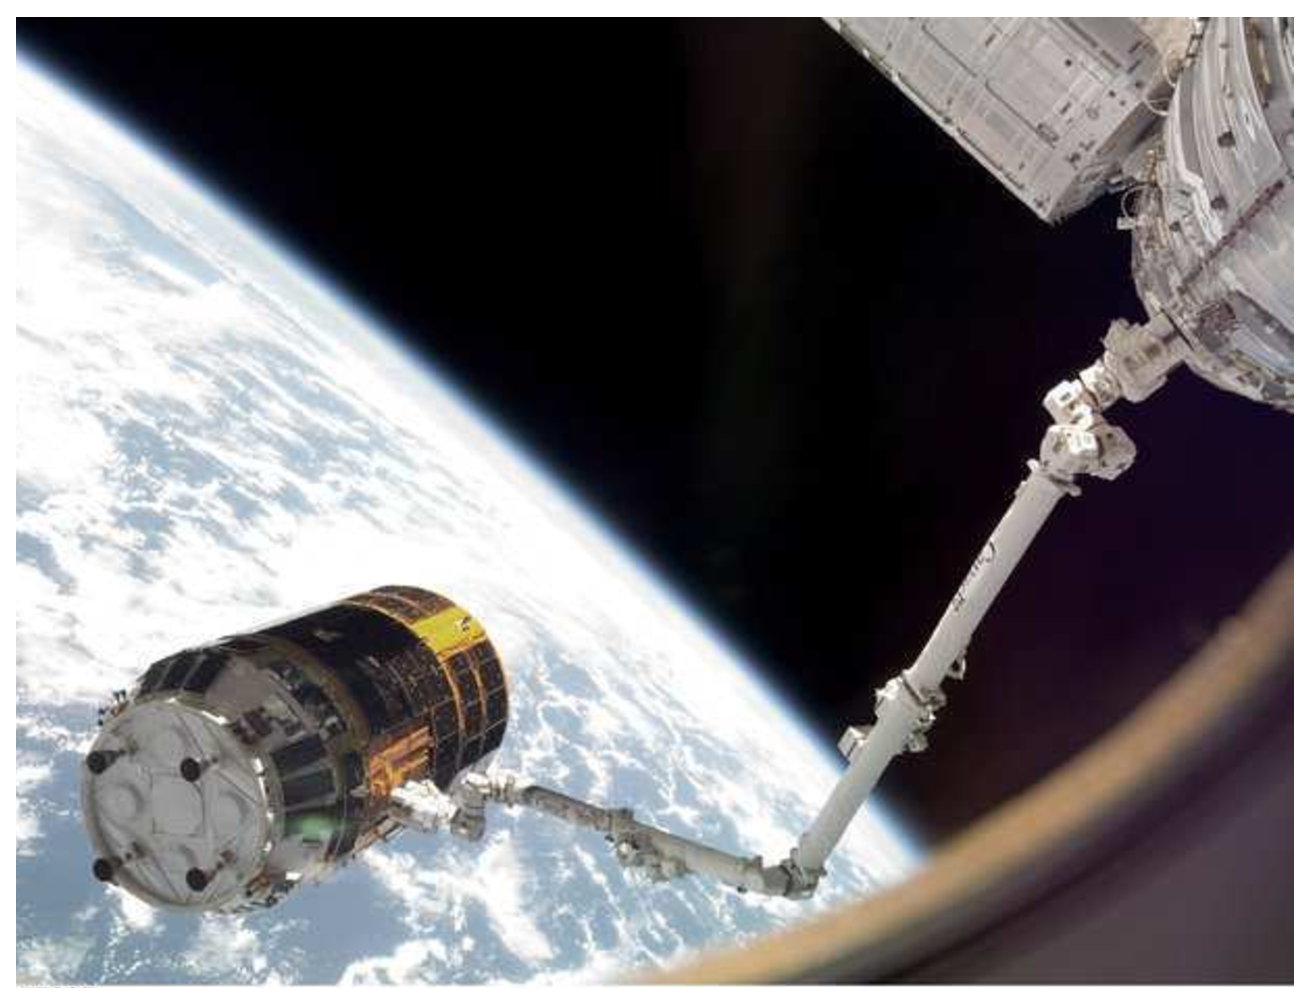
\includegraphics[width=1.0\linewidth]{fig/chapter1/canadarm2.eps}
    \footnotesize\par{(b)}
  \end{minipage}\\
  \vspace{1em}
  \begin{minipage}{0.45\linewidth}
    \centering
    \includegraphics[width=1.0\linewidth]{fig/chapter1/JEMRMS.eps}
    \footnotesize\par{(c)}
  \end{minipage}
  \hspace{2mm}
  \begin{minipage}{0.45\linewidth}
    \centering
    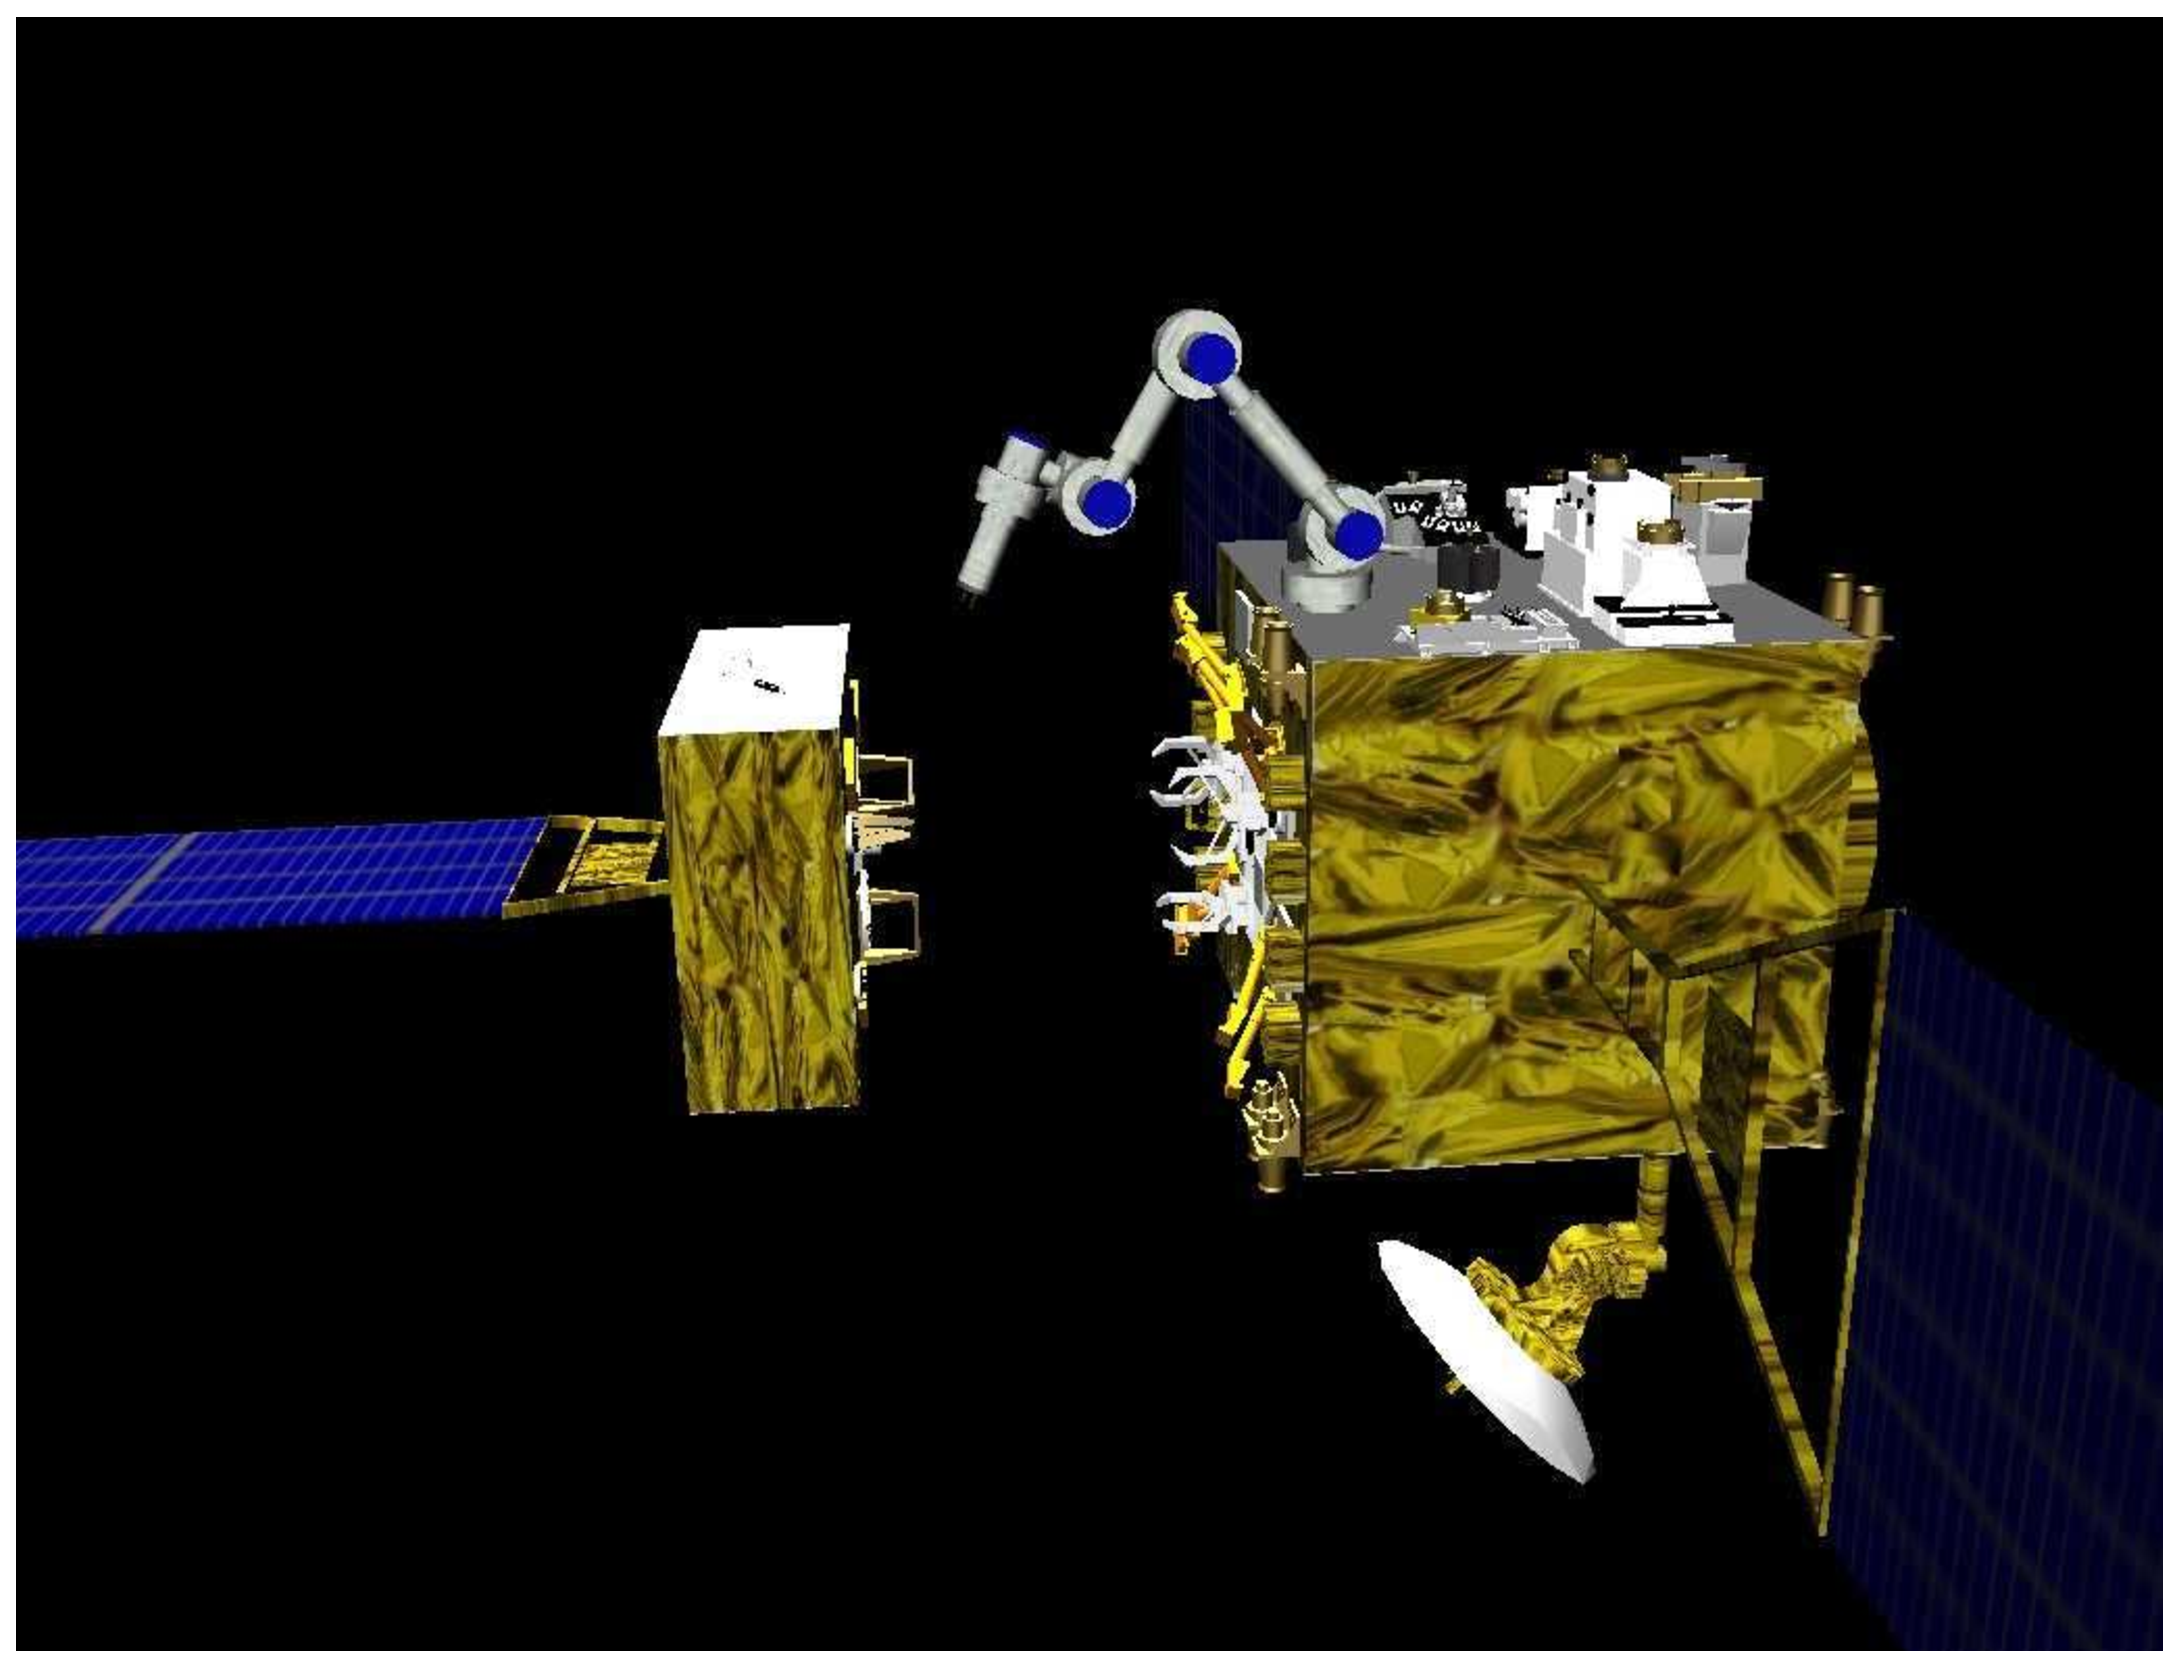
\includegraphics[width=1.0\linewidth]{fig/chapter1/ETSVII.eps}
    \footnotesize\par{(d)}
  \end{minipage}
  \caption{Space robotic systems: (a) Canadarm \copyright NASA, (b) Canadarm 2 \copyright NASA, 
    (c) JEMRMS \copyright JAXA and (d) ETS-VII.}
  \label{fig:SR}
\end{figure}
% ---------------------------------------------------------------------
%

The first use of a robotic system in space is the Shuttle Remote Manipulator System (SRMS),
whose nickname is \textit{Canadarm} (\fig{SR}~(a)),
on Space Shuttle Colombia in 1981 \cite{Flores-Abad2014}.
After that, robotic systems have been employed in various space missions.
A well-known space robot is the Space Station Remote Manipulator System (SSRMS)
developed by the Canadian Space Agency (CSA).
The manipulator was named \textit{Canadarm 2} and has performed several missions, successfully;
the most recent mission executed by Canadarm 2 is a catching mission of the H-II Transfer Vehicle (\fig{SR}~(b)).
Canadarm 2 consists of 17-meter long, 7 degree-of-freedom (DoF) symmetric mechanism.
As a similar robotic system,
the Japan Aerospace Exploration Agency (JAXA) developed the Japanese Experiment Module
Remote Manipulator System (JEMRMS) and a small fine arm (SFA) attached on the end of JEMRMS;
hence, the combined system has been referred to as JEMRMS/SFA (\fig{SR}~(c)).

In addition to this kind of space robotic system,
free-floating space robots (FFSR), which consists of a satellite base and at least one manipulator arm,
are expected to perform future space missions.
These missions would be debris removal, construction of large space buildings,
servicing for launched satellites and so on.
So far, this type of space robots have not been used in practical missions.
% Only experimental systems were developed before.
On the other hand,
an experimental robotic system was developed by JAXA around 1997.
The robotic system has been referred to as the \textit{Experimental Test Satellite VII} (ETS-VII) \cite{Oda1997}.
ETS-VII consists of a 2-meter long, 6-DoF manipulator and a 2000 kg class of unmanned satellite (\fig{SR}~(d)).
The system demonstrated some important robotic technologies:
autonomous rendezvous and docking (AR\&D) and robotic servicing.
The robotic servicing includes exchange of orbital replacement unit (ORU),
deployment of a space structure and capturing of a target satellite.
As an important results,
it was confirmed that the manipulator motions actually induced base motions
as indicated from the mechanics theory \cite{SPACEROBOT,Masutani,Yoshida2003}.
Hence, specific controller designs for space robots
have to be developed in order to execute future space missions, successfully.

%%%%%%%%%%%%%%%%%%%%%%%%%%%%%%%%%%%%%
\subsection{Control issues with FFSR}
%%%%%%%%%%%%%%%%%%%%%%%%%%%%%%%%%%%%%
The most significant problem when controlling manipulators in space
is the dynamic coupling between the manipulators and the satellite base.
The coupling induces a base translation and also rotation.
Because of the base motions,
control methods that have been employed in terrestrial robots cannot be applied straightforwardly.
To overcome this problem,
the information of the base motions has to be taken into account within the control schemes.

An important study considering the above issue was done in \cite{Masutani,Umetani1989}.
The authors proposed the Generalized Jacobian,
which includes a base motion estimated from the linear/angular momentum conservation laws.
By using the Jacobian,
the correct mapping from task space into the joint space can be obtained.
This method can be applied simply by replacing the conventional Jacobian matrix with the generalized one
on the terrestrial robot controllers.
The resolved motion rate control and the resolved acceleration control with the Generalized Jacobian were verified
through numerical simulation.
In addition,
on the experiment with ETS-VII,
the utility of the generalized Jacobian was
confirmed under resolved motion rate control \cite{Yoshida2003}.

On the other hand,
a base rotation itself is a problem because it induces a communication failure between
the space robot and the ground control center.
To overcome this problem,
using gas-jet thrusters were considered by some researchers \cite{Dubowsky1991}.
On the experiment of ETS-VII,
under a camera inspection type of mission,
the thrusters were used to stabilize the base attitude.
However, the fuel for thrusters is finite and its amount determines the life duration of the space systems.
Therefore, attitude devices using electric power such as reaction wheels have been considered so far \cite{Yoshida1994,Aghili2009}.
Reaction wheels have been successfully used on zero momentum type of various satellites
to stabilize their attitude especially against the gravity gradient torque, earth magnetism torque and
solar radiation pressure.
However, if it is considered that reaction wheels are used to compensate
the base reaction induced by a manipulator motion,
the output torque of the reaction wheels is quite insufficient with respect to the base reaction.
To avoid saturation of the reaction wheel signals,
the manipulator has to be driven at very low speed.
When some repeatable tasks, e.g.\ observation/inspection or assembly for construction missions
are performed, this low speed manipulation is
not desirable from the perspective of work efficiency \cite{Umetani1989}.
Hence, developing a control method that generates a manipulator motion inducing a small reaction
is an important issue for space robots.

A pioneering work on manipulator reaction control with free-floating manipulator systems
introduced the Disturbance map concept \cite{Dubowsky1991,Dubowsky1993}.
The base disturbance magnitude is visualized as a colored map in joint space.
With this tool, low reaction paths can be obtained in an intuitive manner.
However, it is difficult to employ this method with manipulators of more than two degrees of 
freedom (DoFs), 
In addition,
it is difficult to obtain a low reaction motion through the color map, automatically.

%%%%%%%%%%%%%%%%%%%%%%%%%%%%%%%%%%%%%%%%%%%
\subsection{Reactionless motion control}
%%%%%%%%%%%%%%%%%%%%%%%%%%%%%%%%%%%%%%%%%%%
A motion generation method was proposed for zero reaction manipulation.
This method has been referred to as the \textit{Reaction Null-Space} (RNS)
formulation \cite{Nenchev1990, Nenchev1999b, Nenchev1999a},
and provides a straightforward approach to reactionless motion generation.
Therein, the condition of reactionless motion was derived from the angular momentum conservation law.
The method was confirmed at the on-orbit experiment with ETS-VII \cite{Yoshida2001}.

In the previous studies,
reactionless motion controls based on RNS have been considered by several researchers \cite{Hirano2014,Oki2007,Hara2010}.
For instance,
the angular momentum distribution control for capturing non-cooperative satellites
under the reactionless condition was proposed \cite{Dimitrov2004}.
The capability of the method was investigated with a planar model.
With a dual arm planar model,
point-to-point (PTP) reactionless motion control was considered for capturing space debris \cite{Shah2013}.
For vibration suppression of flexible appendages on a satellite,
reactionless motion control of the end-effector was considered
in addition to the vibration suppression control \cite{Hirano2014}.
In these studies,
position control of the end-effector under reactionless motion was focused on.
However, the position control between arbitrary locations
would be impossible on general type of spatial manipulators,
e.g.\ six-DoF and seven-DoF redundant manipulators,
due to the limitation of these kinematic structures.
In fact,
the above methods were verified with planar models only.

The possibility of using the RNS method with spatial models is still uncertain, despite 
the reports on some interesting results. For example, within the extended ETS-VII mission,
simple reactionless tasks were examined \cite{Yoshida2000,Yoshida2001}.
Also, results from simulations with a modified ETS-VII manipulator model 
were presented  \cite{Yoshida2001}. In the latter study it was concluded that kinematic redundancy is 
important for the extension of the workspace under reactionless control.
For point-to-point position control, the reaction-null/Jacobian transpose controller
was proposed in \cite{Pisculli2014}. This method was verified with a dual arm 
manipulator system, each manipulator comprising  six DoFs. 
In this work, it was shown that the reachable region of the end-effector from an initial
configuration is quite narrow due to the limitation of the kinematic structure.
On the other hand, a singularity treatment method (the Singularity Consistent approach) 
 was applied to deal with  algorithmic singularities introduced by the reactionless
motion constraint \cite{Nenchev1999c}. It was also confirmed that the workspace of the end-effector 
becomes quit narrow when considering constraints imposed on both end links, the end-effector and the base.
In summary, we can conclude that position control of the end-effector under reactionless control is 
not appropriate in practical tasks even if singularity treatment techniques are used.


%%%%%%%%%%%%%%%%%%%%%%%%%%%%%%%%%%%
\subsection{Energy consumption}
%%%%%%%%%%%%%%%%%%%%%%%%%%%%%%%%%%%
As a different issue in space systems,
energy consumption has been considered.
In the case of controlling satellite attitude,
a power minimization control with redundant reaction wheels were proposed in \cite{Schaub2009}.
From the perspective of tool design,
a low-power image payload was discussed \cite{Carpenter2008,Carpenter2009}.
In that study, Control Moment Gyros (CMG) were employed
because theirs mechanical power/energy is smaller than these produced by a reaction wheel assembly.

On the other hand,
in the field of robotics,
a control method that reduces the energy consumption of free-flying space robots
was proposed \cite{Nakamura1993}.
The study assumed that the base attitude is controlled through four reaction wheels.
Then, the redundant reaction wheel was used to reduce the energy consumption
throughout a manipulator motion.
In \cite{Lampariello2013},
the mechanical power was used as a cost function that is to be minimized.

On reactionless motion control,
the energy optimum reactionless path planning was proposed \cite{Shah20132}.
The method utilized redundancy to optimize the kinetic energy of dual manipulators.
However, a rapid change of the joint velocities was observed due to the optimization.

As mentioned in \cite{Carpenter2008},
reaction wheels require high amount of mechanical power when a large output torque is generated.
Generally, when reaction wheels are used to compensate
the base reaction induced by a manipulator motion,
the reaction wheels must generate a high output torque.
Consequently, the energy consumption becomes large.
On the other hand, reactionless motion control does not necessarily need to use reaction wheels completely.
Hence, it is possible to reduce the energy consumption without
an additional optimization that usually induces unstable behaviors.
The reduction of the energy consumption when using reactionless motion control
has not been discussed before.
In this work,
we focus on the energy consumption reduction and show an interesting result.


%%%%%%%%%%%%%%%%%%%%%%%%%%%%%%%%%%%
\section{Motion/Force control}
%%%%%%%%%%%%%%%%%%%%%%%%%%%%%%%%%%%
With terrestrial robots, force control of the end-effector is as important as motion control.
Especially under interaction tasks,
whose typical examples are polishing, deburring, machining or assembly in industrial settings,
force control providing a compliance behavior
is crucial due to a safe contact between the end-effector of a manipulator and
the unstructured environments.
To understand the importance of the compliance behavior,
we consider a situation that an interaction task is executed by a motion control scheme.
In this case,
the contact between a manipulator and the environment
may cause a deviation of the end-effector motion from the desired trajectory.
Then, an appropriate position feedback controller should intend to reduce the deviation.
As a result,
a built-up of the contact force may occur until causing breakage of a part of the manipulator.
Hence, the compliance behavior of the manipulator end-effector must be needed.

This compliance behavior can be obtained through passive/active interaction control approaches.
The passive approach makes use of a specifically designed
mechanical device such as the Remote Center of Compliance (RCC) device.
This device is designed and has been used for peg-into-hole like tasks.
From the perspective of response time,
the use of a passive device is more suitable than the use of active control approaches.
However, in order to use the passive approach in industrial applications,
specific mechanical devices have to be designed for every robot task.
In addition, the passive devices can only deal with small position and orientation deviations.
Hence, to provide flexibility in robotic tasks,
active interaction control has to be developed.

The active interaction control schemes can be classified into two categories:
indirect force control and direct force control.
Impedance control is a well-known scheme belonging to the first category.
Under impedance control,
the behavior of the end-effector is modeled as an equivalent mass-spring-damper system with
adjustable parameters.
With the model, the contact force of the end-effector
can be related to the deviation of the end-effector motion from the desired one.

On the other hand,
hybrid motion/force control belonging
to the second category has been developed.
The most well-known approach is the so-called \textit{Operational Space} (OS) formulation,
which provides the dynamics of a manipulator in task-space coordinates.
% Using the method can provide a linear and decoupled behavior of the end-effector motion and force.
If the system is non-redundant,
the task-space coordinates are actually the generalized coordinates of the system.
However, with redundant manipulators,
the task-space coordinates cannot be generalized coordinates because there is infinite possibility
providing a relation between the task-space and the joint-space coordinates.
Hence, a suitable transformation between the task-space and joint-space has to be chosen.
To obtain a relation between the two spaces,
the inertia-weighted generalized inverse has been used in various studies \cite{Khatib1987,Park1999,Ott2008,Nakanishi2008}.
The inversion provides a decoupled feature between the task-space and the null-space.
This character is suitable to design task/joint spaces control systems independently of each other.
While task space behavior under the OS formulation (the inertia weighted generalized inverse) seems to be feasible,
unstable behaviors have been observed in joint space \cite{Hollerbach1985,Hollerbach1987}.
In addition, the dynamics of joint-space is to be hidden under the OS formulation.
As a result, the gravity compensation might cause
a cyclic joint motion without affecting the task-space behavior.

Because of these drawbacks of the OS formulation,
we proposed a new motion/force control scheme based on the Reaction Null Space (RNS) formulation,
which has been used for space robots,
especially for redundant manipulators \cite{Hara2012}.
The formulation can represent the dynamics in task-space coordinates without
making use of a transformation between the two spaces.
In addition, the joint motion is explicitly presented in the task-space dynamics.
Comparing with the OS formulation,
we confirmed that the RNS-based control would have an advantages in terms of joint motion \cite{Hara2012}.
In this work, we provide a depth discussion of the joint motion under the RNS-based control that
has been unclear so far.


%%%%%%%%%%%%%%%%%%%%%%%%%%%%%
\section{Aim of this study}
%%%%%%%%%%%%%%%%%%%%%%%%%%%%%
This thesis treats the following two topics for the RNS-based controls:
(i) reactionless motion control for free-floating space robots and
(ii) motion/force control for fixed-base redundant manipulators.

On reactionless motion control of free-floating space robots,
we discuss the following issues:
%
\begin{description}
\item[i-1] Analysis of reactionless motion from the perspective of nonlinear dynamics.
\item[i-2] Proposal of some practical tasks suitable for execution under reactionless motion control.
\item[i-3] Analysis of the energy consumption under reactionless motion control.
\end{description}
%

On the RNS-based motion/force control,
we treat the following topics:
\begin{description}
\item[ii-1] Obtain a specific model for the RNS-based motion/force control.
\item[ii-3] Clarify the joint motion under the RNS-based motion/force control.
\end{description}


%%%%%%%%%%%%%%%%%%%%%%%%%%%%%%%%%%
\section{Outline of this thesis}
%%%%%%%%%%%%%%%%%%%%%%%%%%%%%%%%%%
This thesis consists of the eight chapters as follows:
\cha{BASIC} describes the modeling of free-floating base robot systems.
The equation of motion of the system is derived from the Euler-Lagrange's equation.
Then, linear and angular momentum conservation laws are
derived via considering the invariance of the system Lagrangian 
with translation and rotation of the entire system.
Finally, we present the Reaction Null-Space formulation
in terms of both momentum and dynamics.

In Chapters \ref{cha:ANALYSIS} to \ref{cha:ENERGY},
we deal with reactionless motion control of free-floating space robots.
In \cha{ANALYSIS},
we provide an analysis of reactionless motion with a planar two-DoF model
from the perspective of nonlinear dynamics:
vector field, fixed point and bifurcation.
Besides, with a seven-DoF redundant manipulator,
we obtain a representation of its reactionless motion that is useful to consider
for practical reactionless tasks.

\cha{PROPOSAL} discusses motion tasks suitable for execution
under reactionless motion control.
We propose the following three tasks:
(i) inspection task using a hand camera,
(ii) point-to-point positioning task,
(iii) deployment task from a stowed configuration.
The performance of these tasks is verified via numerical simulations.

In \cha{ENERGY}, we deal with the energy consumption of free-flying space robots,
comparing that produced by reactionless motion control with that produced by reaction wheels used controllers.
Under zero base attitude deviation,
we show that reactionless motion coincides with the instantaneous energy minimum motion to a high degree.
Then, the energy consumption of reactionless motion control is compared
with a conventional controller using reaction wheels under the inspection tasks.

In the next two chapters,
we deal with the motion/force control based on the Reaction Null-Space for fixed base redundant manipulators.
In \cha{FORMULATION},
we formulate the RNS-based motion/force control.
Then, a specific model for the RNS-based controller is presented.
Finally, the performance of the proposed method is verified through numerical simulation.

\cha{JOINT} discusses the joint motion under the RNS-based motion/force control.
We show an interesting fact that the joint motion under the RNS-based controller
is equivalent to that under the resolved acceleration control.
The theoretical derivation and numerical verification are obtained.

Finally, \cha{CONCLUSION} summarizes this thesis.

%%%%%%%%%%%%%%%%%%%%%%%%%%%%%%%%%%%%%%%%%%%%
\section{The roles of variable's index}
%%%%%%%%%%%%%%%%%%%%%%%%%%%%%%%%%%%%%%%%%%%%
Basically, we describe vectors and matrices according to the following roles of the indexes.
\textit{Left superscript}: reference frames in which quantities are described.
\textit{Right superscript}: conditions of variables,
  e.g.\ $T$ (Transposed), $-1$ (Inversion), $des$ (Desired), $ref$ (Reference) and so on.
\textit{Right subscript} physical quantities, component, manipulator mechanisms and so on.

We provide two examples according to the above roles, in what follows.
First, we consider the Jacobian $\bm{J}$ associated with end-effector linear velocity $\bm{v}_{e}$
with respect to the inertial coordinate frame $\{F\}$.
This matrix is written as ${}^{F}\bm{J}_{v_{e}}$.

Next, we consider the same Jacobian but it just consists of the positioning subchain $P$,
which is a specific part of a manipulator mechanism.
This matrix is written as ${}^{F}\bm{J}_{Pv_{e}}$.
Note that if we consider the whole mechanism of a manipulator,
we omit this notation.

If we describe relative quantities such as position, velocity,
we will make use of the following notation:
$\bm{r}_{A \rightarrow B}$ representing a position vector pointing to the position $B$
with respect to $A$.
Note that the notation of the inertial coordinate frame is omitted in all quantities appearing below.



%**********************************************************************
%
%
%%% Local Variables:
%%% mode: latex
%%% TeX-master: "./main"
%%% End:

\chapter{Basic Notation}
\label{cha:BASIC}
% Abstract for this chapter
%
%**********************************************************************


In this section, we describe the equation of motion of a free-floating base robot.
We derive the equation through the Euler-Lagrange's equation.
Then, we show that the linear/angular conservation laws, which play an important role in robotics,
can be derived from the equation of motion
with assuming invariance of the system Lagrangian under translation and rotation of the entire system.
From linear/angular momentum conservation laws,
we obtain the Reaction Null-Space formulation that 
is useful for reactionless motion control of space robots
and also motion/force control of redundant manipulators.


%%%%%%%%%%%%%%%%%%%%%%%%%%%%%%%%%%%%%%%%%%%%%%%%%%%%%%%%%%%%%%%
\section{Modeling of free-floating base robots}
%%%%%%%%%%%%%%%%%%%%%%%%%%%%%%%%%%%%%%%%%%%%%%%%%%%%%%%%%%%%%%%
%
% ---------------------------------------------------------------------
\begin{figure}[t]
  \centering
  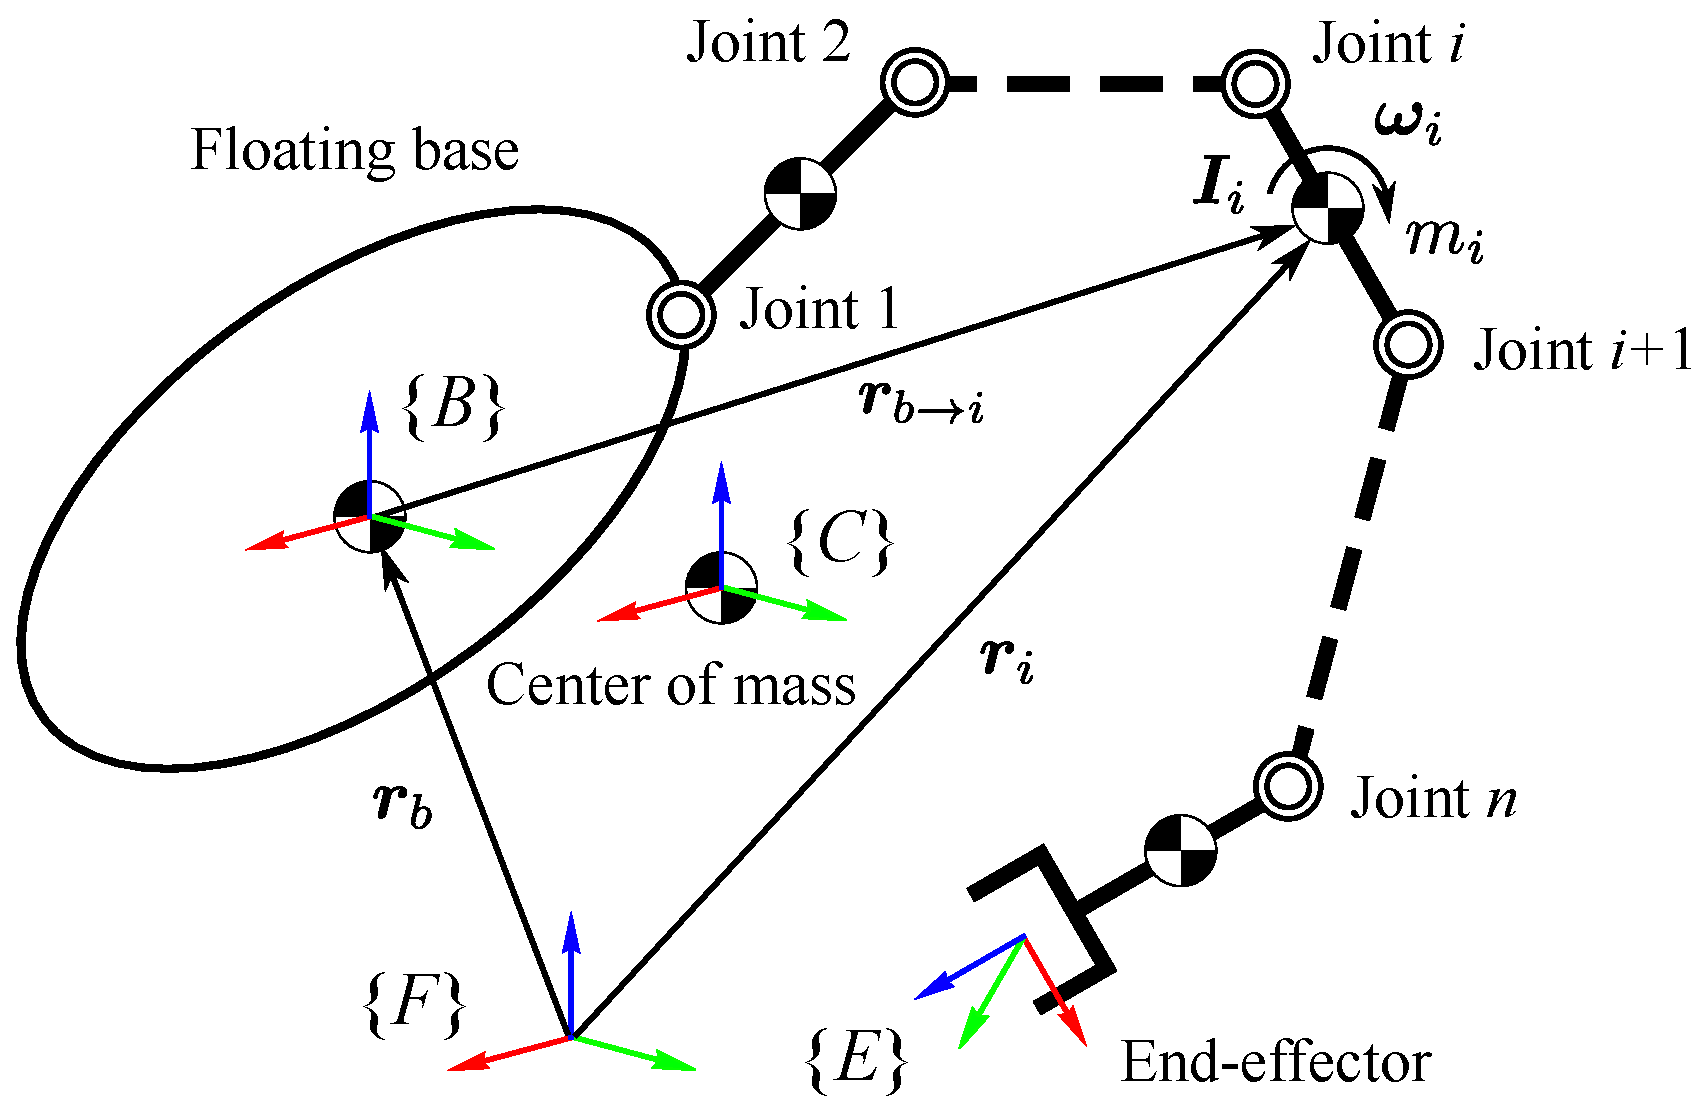
\includegraphics[width=0.7\linewidth]{fig/chapter2/FFSM.eps}
  \caption{General model of free-floating base robot.}
  \label{fig:MODEL_FFSM}
\end{figure}
% ---------------------------------------------------------------------
%
We consider a free-floating base robot 
that consists of a floating base and links, e.g.\ manipulators and reaction wheels,
as shown in \fig{MODEL_FFSM}.
Let us define the inertial coordinate frame $\{F\}$.
% Traditionally, it is considered that the coordinate frame can be moved along the orbit with constant speed.
We use two kind of position vector.
One of them is vector from the inertial frame;
the other is one from the base coordinate frame $\{B\}$.
Note that, except special cases these vectors are described with respect to the inertial frame.


Here, we introduce generalized coordinate to describe the system dynamics.
The coordinate is defined as $\bm{q} = [\mathcal{X}_{b}^{T}~\th^{T}]^{T}\R{n + 6}$,
where $\mathcal{X}_{b} = [\bm{r}_{b}^{T}~\bm{\xi}_{b}^{T}]^{T}\R6$ stands for the base variables:
$\bm{r}_{b}\R3$ and $\bm{\xi}_{b}$ are base position vector and Euler angle describing the base attitude;
especially we make use of Roll-Pitch-Yaw angle.
$\th\R{n}$ is the joint variable vector.
Note that because of the non-integrability of angular velocity,
the base spatial velocity $\mathcal{V}_{b} = [\bm{v}_{b}^{T}~\bm{\omega}_{b}^{T}]^{T}$ cannot be obtained
as the time-differential of $\mathcal{X}_{b}$.
Hence, an appropriate transformation between the time-differential of the Euler angle and the angular velocity is needed:
%
% ---------------------------------------------------------------------
\begin{align}
  \dot{\bm{\xi}}_{b} = \bm{A}^{-1}\bm{\omega}_{b}
\end{align}
% ---------------------------------------------------------------------
%
where $\bm{A}\R{3 \times 3}$ is the transformation matrix.




%%%%%%%%%%%%%%%%%%%%%%%%%
\subsection{Kinematics}
%%%%%%%%%%%%%%%%%%%%%%%%%
Seen from \fig{MODEL_FFSM},
the position vector of each link can be written as follows:
%
% ---------------------------------------------------------------------
\begin{align}
  \bm{r}_{i} = \bm{r}_{b} + \bm{r}_{b \rightarrow i}\label{eq:POS_LINKi}
\end{align}
% ---------------------------------------------------------------------
%
where $\bm{r}_{i}$, $\bm{r}_{b \rightarrow i}$ are the position vectors pointing to the center of mass of each link
from the inertial frame and the base frame, respectively.
Differentiating \eq{POS_LINKi} with respect to time $t$,
we can obtain the differential kinematic equation:
%
% ---------------------------------------------------------------------
\begin{align}
  \bm{v}_{i} = \bm{v}_{b} + \bm{J}_{v_{i}}(\bm{q})\thd + [\bm{\omega}_{b}^{\times}]\bm{r}_{b \rightarrow i}\label{eq:VEL_LINKi}
\end{align}
% ---------------------------------------------------------------------
%
where $\bm{v}_{i}$ stands for linear velocity of link $i$,
$\bm{v}_{b}$, $\bm{\omega}_{b}\R3$ are linear and angular velocities of the base.
$\bm{J}_{v_{i}}(\bm{q})\R{3 \times n}$ is the Jacobian for linear velocity of the link $i$ CoM.
$\dot{(\circ)}$ and $(\circ)^{\times}$ define time differential and skew-symmetric matrix.

In contrast to the linear velocity equation,
the kinematic equation of angular velocity cannot be obtained directly
as the time differential of the position-level equation because of its non-integrability.
The angular velocity of link $i$ is expressed in the following form:
%
% ---------------------------------------------------------------------
\begin{align}
  \bm{\omega}_{i} = \bm{\omega}_{b} + \bm{J}_{\omega_{i}}(\bm{q})\thd\label{eq:ANGVEL_LINKi}
\end{align}
% ---------------------------------------------------------------------
%
where $\bm{\omega}_{i}$ stands for angular velocity of link $i$,
$\bm{J}_{\omega_{i}}(\bm{q})\R{3 \times n}$ is the Jacobian associated with the angular velocity of link $i$.

% For description convenience,
% we introduce spatial velocity $\mathcal{V}_{i} = [\bm{v}_{i}^{T}~\bm{\omega}_{i}^{T}]^{T}$.
% Through the notation,
% the generalized velocity vector can be expressed as $\dot{\bm{q}} = [\mathcal{V}_{b}^{T}~\thd^{T}]^{T}$, hereafter.
% It should be noted that we use Euler angle to represent the orientation of the base
% because of the non-integrability of angular velocity,



%%%%%%%%%%%%%%%%%%%%%%%%%%%%
\subsection{Kinetic energy}
%%%%%%%%%%%%%%%%%%%%%%%%%%%%
The kinetic energy of the free-floating base robots is represented as follows:
%
% ---------------------------------------------------------------------
\begin{align}
  T = \frac{1}{2}\sum_{i = 0}^{n}(m_{i}\bm{v}_{i}^{T}\bm{v}_{i} + \bm{\omega}_{i}^{T}\bm{I}_{i}\bm{\omega}_{i})
  \label{eq:ENERGY_GEN}
\end{align}
% ---------------------------------------------------------------------
%
where $T$ is kinetic energy,
$m_{i}$ and $\bm{I}_{i}\R3$ are the mass and the inertia tensor of each link.
Substituting \eq{VEL_LINKi} and \eq{ANGVEL_LINKi} into the above equation,
we can rewrite the kinetic energy in terms of the base and the joint variables:
%
% ---------------------------------------------------------------------
\begin{align}
  T &= \frac{1}{2}\dot{\bm{q}}^{T}\bm{M}(\bm{q})\dot{\bm{q}}\\
  &= \frac{1}{2}\bmat{\mathcal{V}_{b}^{T} & \thd^{T}}\bmat{\bm{M}_{b}(\bm{q}) & \bm{M}_{bl}(\bm{q}) \\
    \bm{M}_{bl}(\bm{q})^{T} & \bm{M}_{l}(\bm{q})}
  \bmat{\mathcal{V}_{b} \\ \thd}\label{eq:ENERGY}
\end{align}
% ---------------------------------------------------------------------
%
where $\bm{M}(\bm{q})\R{(n+6)\times (n+6)}$ is the inertia matrix of the entire mechanism.
$\bm{M}_{b}(\bm{q})\R{6 \times 6}$,
$\bm{M}_{bl}(\bm{q})\R{6 \times n}$ and $\bm{M}_{l}(\bm{q})\R{n \times n}$ are the submatrices of the inertia matrix;
$\bm{M}_{b}$ is the inertia matrix of the system regarded as a Composite-Rigid-Body (CRB),
$\bm{M}_{bl}$ is a block submatrix of the system inertia matrix.
This matrix represents a dynamic coupling between base motion and link motion.
Hence, it has been referred to as the \textit{coupling inertia} matrix,
and plays an important role under controlling space robots.
Finally, $\bm{M}_{l}$ denotes the manipulator inertia matrix.

%%%%%%%%%%%%%%%%%%%%%%%%%%%%%%%%%%
\subsection{Inertia submatrices}
%%%%%%%%%%%%%%%%%%%%%%%%%%%%%%%%%%
Here, we provide the definitions of the inertia submatrices.
The matrix $\bm{M}_{b}$ is defined in the following form:
%
% ---------------------------------------------------------------------
\begin{align}
  \bm{M}_{b} &= \bmat{\bm{M}_{v} & \bm{M}_{v\omega} \\ \bm{M}_{v\omega}^{T} & \bm{M}_{\omega}}\\
  \bm{M}_{v} &= m_{C}\bm{E}\\
  \bm{M}_{v\omega} &= -\sum_{i=1}^{n}m_{i}[\bm{r}_{b \rightarrow i}^{\times}]\\
  \bm{M}_{\omega} &= \sum_{i=1}^{n}(\bm{I}_{i} + m_{i}[\bm{r}_{b \rightarrow i}^{\times}]^{T}[\bm{r}_{b \rightarrow i}^{\times}]) + \bm{I}_{b}
\end{align}
% ---------------------------------------------------------------------
%
where $m_{C} = \sum_{i=0}^{n}m_{i}$ is the total mass of the system,
$m_{i}$ and $\bm{I}_{i}\R3$ is the mass and the inertia tensor of link $i$.
$\bm{E}\R{3 \times 3}$ is the identity matrix.

The coupling inertia matrix $\bm{M}_{bl}$ is defined as follows:
%
% ---------------------------------------------------------------------
\begin{align}
  \bm{M}_{bl} &= \bmat{\bm{M}_{vl} \\ \bm{M}_{\omega l}}\\
  \bm{M}_{vl} &= \sum_{i = 1}^{n}m_{i}\bm{J}_{v_{i}} = m_{C}\bm{J}_{C}\\
  \bm{M}_{\omega l} &= \sum_{i = 1}^{n}(\bm{I}_{i}\bm{J}_{\omega_{i} } + m_{i}[\bm{r}_{b \rightarrow i}^{\times}]\bm{J}_{v_{i}})
\end{align}
% ---------------------------------------------------------------------
%
where $\bm{J}_{C}\R{3\times n}$ is the Jacobian matrix for the CoM velocity of the system;
hence it is referred to as the CoM Jacobian.

Finally, $\bm{M}_{l}$ is described as follows:
%
% ---------------------------------------------------------------------
\begin{align}
  \bm{M}_{l} = \sum_{i=1}^{n}(m_{i}\bm{J}_{v_{i}}^{T}\bm{J}_{v_{i}} + \bm{J}_{\omega_{i}}^{T}\bm{I}_{i}\bm{J}_{\omega_{i}})
\end{align}
% ---------------------------------------------------------------------
%
Note that this matrix is the same as the manipulator inertia matrix of fixed base robots.


%%%%%%%%%%%%%%%%%%%%%%%%%%%%%%%%%
\subsection{Equation of motion}
%%%%%%%%%%%%%%%%%%%%%%%%%%%%%%%%%
Since we consider free-floating systems,
the gravity potential is approximately zero.
Hence, the system Lagrangian coincides with the kinetic energy:
%
% ---------------------------------------------------------------------
\begin{align}
  L(\bm{q},\dot{\bm{q}}) = T(\bm{q},\dot{\bm{q}})\label{eq:LAGRANGIAN}
\end{align}
% ---------------------------------------------------------------------
%
where $L(\q,\qd)$ is the system Lagrangian.

From the theory of analytical mechanics,
equation of motions of dynamic system can be obtained
from the partial derivation of the system Lagrangian.
Then, equation of motions satisfy the following equation:
%
% ---------------------------------------------------------------------
\begin{align}
  \frac{d}{dt}(\PD{L}{\dot{\bm{q}}}) - \PD{L}{\bm{q}} = \bm{Q}\label{eq:LAGRANGE_EQ}
\end{align}
% ---------------------------------------------------------------------
%
where $\bm{Q}$ is generalized force vector acting on each generalized coordinate.

Substituting \eq{ENERGY} and \eq{LAGRANGIAN} into \eq{LAGRANGE_EQ},
we can obtain the equation of motion of a free-floating base robot in the following form:
%
% ---------------------------------------------------------------------
\begin{align}
  \bm{M}_{b}\dot{\mathcal{V}}_{b} + \bm{M}_{bl}\thdd + \mathcal{C}_{b} &= \bm{0}\label{eq:EOM_BASE}\\
  \bm{M}_{bl}^{T}\dot{\mathcal{V}}_{b} + \bm{M}_{l}\thdd + \bm{c}_{l} &= \bm{\tau}\label{eq:EOM_LINK}
\end{align}
% ---------------------------------------------------------------------
%
where $\bm{\tau}\R{n}$ is joint torque acting on each joint,
$\mathcal{C}_{b}\R{6}$ and $\bm{c}_{l}\R{n}$ are nonlinear
dependent forces of the base and the links.
These nonlinear forces are represented in the following form:
%
% ---------------------------------------------------------------------
\begin{align}
  \bm{c} = \bmat{\mathcal{C}_{b} \\ \bm{c}_{l}} =
  \dot{\bm{M}}\thd - \frac{1}{2}\PD{}{\bm{q}}\Big(\dot{\bm{q}}^{T}\bm{M}\dot{\bm{q}}\Big)
\end{align}
% ---------------------------------------------------------------------
%

Equation \eq{EOM_BASE} represents the dynamics of the composite rigid-body (CRB);
\eq{EOM_LINK} describes the same dynamics with respect to the local coordinate frames.

%%%%%%%%%%%%%%%%%%%%%%%%%%%%%%%%%%%%%%%%%%%
\section{Momentum conservation law}
%%%%%%%%%%%%%%%%%%%%%%%%%%%%%%%%%%%%%%%%%%%
%%%%%%%%%%%%%%%%%%%%%%%%%%%%%%%%%%%%%%%%%%%
\subsection{Linear momentum conservation law}
%%%%%%%%%%%%%%%%%%%%%%%%%%%%%%%%%%%%%%%%%%%

In the field of robotics,
linear and angular momenta and their conservation laws play an important role.
In particular, these provide the reactionless motion constraint for space robots;
in the field of humanoids,
these are used to built balancing controllers and also whole body motion controllers.
Considering the invariance of the system Lagrangian under variations of position and rotation of a dynamic system,
we can obtain the conservation laws in what follows.

First, we derive the linear momentum conservation law of free-floating base robots.
Empirically,
we know that physical laws is not changed with translation of dynamic systems;
the translation indicates that the whole part of the system move in the same direction, simultaneously.

We assume that the system consists of $n+1$ bodies like manipulator mechanisms.
The position vectors pointing to each body are defined as $\bm{r}_{i}$.
Then, under a variation of translation $\delta \bm{r}_{i}$,
the variation of the system Lagrangian can be written as follows:
%
% ---------------------------------------------------------------------
\begin{align}
  \delta L = \sum_{i = 0}^{n}\PD{L}{\bm{r}_{i}}\delta \bm{r}_{i}
\end{align}
% ---------------------------------------------------------------------
%
Because the variation of the Lagrangian muse be zero with an arbitrary value of $\delta \bm{r}_{i}$,
the following condition must satisfy:
%
% ---------------------------------------------------------------------
\begin{align}
  \sum_{i=0}^{n}\PD{L}{\bm{r}_{i}} = \bm{0}
\end{align}
% ---------------------------------------------------------------------
%
According to \eq{LAGRANGE_EQ},
the above condition is equivalent to the following equation:
%
% ---------------------------------------------------------------------
\begin{align}
  \sum_{i=0}^{n}\frac{d}{dt}(\PD{L}{\dot{\bm{r}}_{i}}) = \bm{0}\label{eq:LINEAR_GEN}
\end{align}
% ---------------------------------------------------------------------
%
where $\sum\PD{L}{\dot{\bm{r}}_{i}}$ is an invariable and 
$\bm{p}_{i} = \PD{L}{\dot{\bm{r}}_{i}}$ is defined as \textit{linear momentum}.
Hence, \eq{LINEAR_GEN} represents the linear momentum conservation law.
Using the same expression of \eq{ENERGY_GEN},
the conservation law can be written in the following well-known form:
%
% ---------------------------------------------------------------------
\begin{align}
  \bm{p} = \sum_{i=0}^{n}m_{i}\bm{v}_{i}
\end{align}
% ---------------------------------------------------------------------
%
In the case of free-floating base robots,
a variation of translation can be considered as the base position vector $\delta \bm{r}_{b}$.
Then, the linear momentum conservation law of free-floating base robots can be obtained as:
%
% ---------------------------------------------------------------------
\begin{align}
  \frac{d}{dt}(\PD{L}{\bm{v}_{b}}) = \bm{0}\label{eq:LINE_MOM_LAW}
\end{align}
% ---------------------------------------------------------------------
%
This is equivalent to the following equation:
%
% ---------------------------------------------------------------------
\begin{align}
  \bm{p} = \bm{M}_{v}\bm{v}_{b} + \bm{M}_{v\omega}\bm{\omega}_{b} + \bm{M}_{vl}\thd
\end{align}
% ---------------------------------------------------------------------
%
The above expression of the conservation law has been used in various studies.

%%%%%%%%%%%%%%%%%%%%%%%%%%%%%%%%%%%%%%%%%%%%%%%%%%%%%
\subsection{Angular momentum conservation law}
%%%%%%%%%%%%%%%%%%%%%%%%%%%%%%%%%%%%%%%%%%%%%%%%%%%%%
%
% ---------------------------------------------------------------------
\begin{figure}[t]
  \centering
  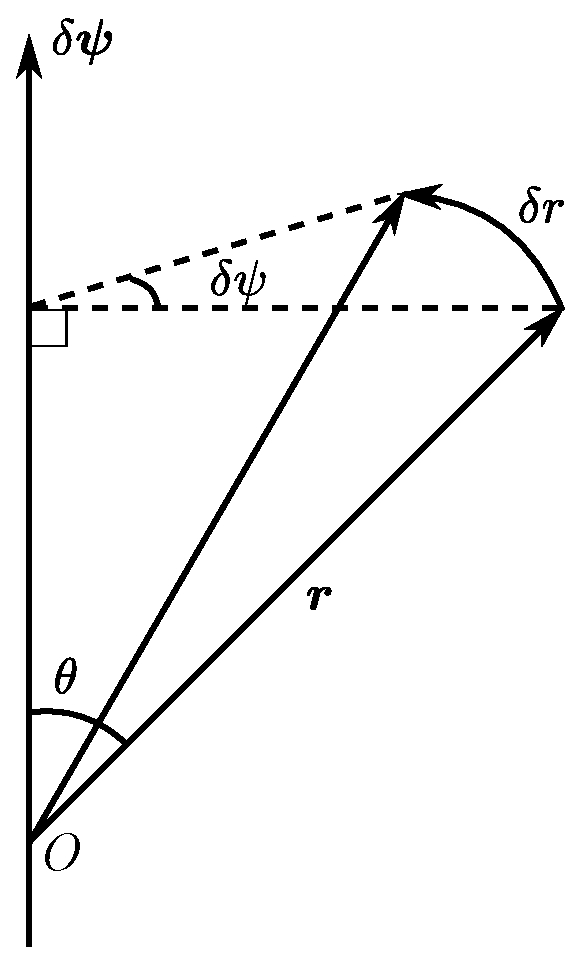
\includegraphics[width=0.3\linewidth]{fig/chapter2/rotation.eps}
  \caption{Relationship between a variation of translation and a rotational variation.}
  \label{fig:ROT}
\end{figure}
% ---------------------------------------------------------------------
%
We derive the angular momentum conservation law of free-floating base robots.
In contrast to linear momentum conservation law,
angular momentum conservation law is obtained from invariance of the system Lagrangian
under an infinitesimal rotation of dynamic systems.

First, we derive, also, the general form of angular momentum conservation law.
We introduce an infinitesimal rotation vector $\delta\bm{\psi}$.
Then, a position vector pointing to an arbitrary particle of a rotating system
varies according to $\delta \bm{\psi}$.
The position variation is written as follows (see \fig{ROT}):
%
% ---------------------------------------------------------------------
\begin{align}
  \|\delta \bm{r}\| = r\sin\alpha\|\delta\bm{\psi}\|
\end{align}
% ---------------------------------------------------------------------
%
Under an arbitrary infinitesimal rotation,
the velocity of each body also varies.
The variation of the velocity is written as:
%
% ---------------------------------------------------------------------
\begin{align}
  \delta \bm{v} = \delta\bm{\psi}\times \bm{v}
\end{align}
% ---------------------------------------------------------------------
%

With the above relation,
the variation of the system Lagrangian under an infinitesimal rotation can be written as:
%
% ---------------------------------------------------------------------
\begin{align}
  \delta L &= \sum_{i=0}^{n}\Big\{\dot{\bm{p}}_{i}(\delta{\bm{\psi}}^{T}\bm{r}_{i}) +
  \bm{p}_{i}(\delta\bm{\psi}^{T}\bm{v}_{i})\Big\}\notag\\
  &= \delta\bm{\psi}\frac{d}{dt}\sum_{i=0}^{n}\bm{r}_{i}\times\bm{p}_{i}\notag\\
  &= 0
\end{align}
% ---------------------------------------------------------------------
%
Because $\delta\bm{\psi}$ can be an arbitrary value,
the following condition muse be satisfied:
%
% ---------------------------------------------------------------------
\begin{align}
  \frac{d}{dt}\sum_{i=0}^{n}\bm{r}_{i}\times\bm{p}_{i} = \bm{0}
\end{align}
% ---------------------------------------------------------------------
%
Hence, we found out that the quantity $\sum\bm{r}_{i}\times\bm{p}_{i}$ conserves;
$\bm{l}_{Fi} = \bm{r}_{i}\times \bm{p}_{i}$ is defined as \textit{angular momentum},
where $(\circ)_{F}$ represent the angular momentum with respect to the inertial frame $\{F\}$.
Using the same expression of \eq{ENERGY_GEN},
we can rewrite the angular momentum conservation law in the following form:
%
% ---------------------------------------------------------------------
\begin{align}
  \bm{l}_{F} = \sum_{i=0}^{n}\Big\{\bm{I}_{i}\bm{\omega}_{i} + m_{i}\bm{r}_{i}\times \bm{v}_{i}\Big\}
\end{align}
% ---------------------------------------------------------------------
%
In the case of free-floating robots,
this equation can be expressed as:
%
% ---------------------------------------------------------------------
\begin{align}
  \bm{l}_{F} = \bm{M}_{v\omega}^{T}\bm{v}_{i} + \bm{M}_{\omega}\bm{\omega}_{b} + \bm{M}_{\omega l}\thd
  + \bm{r}_{b}\times \bm{p}
\end{align}
% ---------------------------------------------------------------------
%

% Summary, momenta conservation laws of free-floating robots can be written as follows:
% %
% % ---------------------------------------------------------------------
% \begin{align}
%   \bmat{\bm{p} \\ \bm{l}_{B}} =
%   \bm{M}_{b}\mathcal{V}_{b} + \bm{M}_{bl}\thd + \bmat{\bm{0} \\ \bm{r}_{b} \times \bm{p}}
%   \label{eq:SPATIAL_MOM}
% \end{align}
% % ---------------------------------------------------------------------
% %



% %%%%%%%%%%%%%%%%%%%%%%%%%%%%%%%%%%%%%%%%%%%%%%%
% \subsection{The momenta conservation law}
% %%%%%%%%%%%%%%%%%%%%%%%%%%%%%%%%%%%%%%%%%%%%%%%


%%%%%%%%%%%%%%%%%%%%%%%%%%%%%%%%%%%%%%%%%%%%
\section{Reaction Null-Space}
%%%%%%%%%%%%%%%%%%%%%%%%%%%%%%%%%%%%%%%%%%%%
Reaction Null-Space was originally proposed for
reactionless motion control of space robots.
With the ETS-VII experiment,
the possibility of reactionless motion control was confirmed.
In what follows, we describe the Reaction Null-Space formulation in terms of both momentum and dynamics.

%%%%%%%%%%%%%%%%%%%%%%%%%%%%%%%%%%%%%%%%%%%%
\subsection{Momentum based derivation}
%%%%%%%%%%%%%%%%%%%%%%%%%%%%%%%%%%%%%%%%%%%%
The spatial momentum conservation law is obtained in the following form:
%
% ---------------------------------------------------------------------
\begin{align}
  \mathcal{L}_{B} = \bm{M}_{b}\mathcal{V}_{b} + \bm{M}_{bl}\thd\label{eq:SPA_MOM}
\end{align}
% ---------------------------------------------------------------------
%
where $\mathcal{L}_{B} = [\bm{p}^{T}~\bm{l}_{B}^{T}]^{T}$ is spatial momentum with respect to the base frame $\{B\}$.
From the above equation,
we can confirm that there are two partial momenta:
$\bm{M}_{b}\mathcal{V}_{b}$ represents the partial momentum related to base motion;
$\bm{M}_{bl}\thd$ is stemming from manipulator motion.
In particular, the later one has been referred to as the \textit{coupling momentum},
and is characterized by the coupling inertia matrix.

Solving \eq{SPA_MOM} for joint velocity,
we can obtain a joint-space decomposition in terms of the dynamic coupling as follows:
%
% ---------------------------------------------------------------------
\begin{align}
  \thd = \bm{M}_{bl}^{+}(\mathcal{L}_{B} - \bm{M}_{b}\mathcal{V}_{b}) + \bm{P}_{RNS}\thd_{a}\label{eq:RNS_VEL}
\end{align}
% ---------------------------------------------------------------------
%
where $(\circ)^{+}$ defines pseudoinverse matrix,
$\bm{P}_{RNS} = \bm{E} - \bm{M}_{bl}^{+}\bm{M}_{bl}\R{n \times n}$ is the projector onto the null-space of
the coupling inertia matrix.
$\thd_{a}\R{n}$ is an arbitrary vector with dimensions of joint velocity.
The first term represents joint velocities inducing a base motion;
on the other hand,
the second term does not impose any motion at the base.
Hence, the motions are referred to as \textit{reactionless motion}.
Since the property of pseudoinverse,
the above two terms are orthogonal with any values of $(\mathcal{L}_{B} - \bm{M}_{b}\mathcal{V}_{b})$ and
$\thd_{a}$.
This joint space decomposition has been referred to as
\textit{Reaction Null-Space} in terms of momentum.


%%%%%%%%%%%%%%%%%%%%%%%%%%%%%%%%%%%%%%%%%%
\subsection{Dynamics based derivation}
%%%%%%%%%%%%%%%%%%%%%%%%%%%%%%%%%%%%%%%%%%
Let us recall the equation of motion \eq{EOM_BASE}, as follows:
%
% ---------------------------------------------------------------------
\begin{align}
  \bm{M}_{b}\dot{\mathcal{V}}_{b} + \bm{M}_{bl}\thdd + \mathcal{C}_{b} &= \bm{0}
\end{align}
% ---------------------------------------------------------------------
%
From the above equation, we can also see that there is
a coupling between the base dynamics and the manipulator one
through the coupling inertia matrix.
Through the same approach under the momentum-based derivation,
the Joint dynamics can be divided into two parts in the following form:
%
% ---------------------------------------------------------------------
\begin{align}
  \thdd = \bm{M}_{bl}^{+}(\bm{M}_{b}\dot{\mathcal{V}}_{b} - \mathcal{C}_{b}) + \bm{P}_{RNS}\thd_{a}\label{eq:RNS_ACC}
\end{align}
% ---------------------------------------------------------------------
%
The first term on the r.h.s.\ represents joint accelerations inducing a base motion,
the second term defines reactionless acceleration, whose meaning is the same as the momentum derivation.
Note that the motions of \eq{RNS_VEL} and \eq{RNS_ACC} are not basically equivalent,
since there is non-integrability between the two formulations;
this non-integrability is due to the pseudoinverse.


%%%%%%%%%%%%%%%%%%%%%
\section{Summary}
%%%%%%%%%%%%%%%%%%%%%
In this section, we described the equation of motion of a free-floating base robots
from the Euler-Lagrange formulation.
We showed the two important conservation laws, which are linear and angular momentum conservation law,
with assuming invariance of the system Lagrangian under variation of position and orientation of dynamic systems.
Then, we derived the Reaction Null-Space formulation with dimensions of both momentum and dynamics.
Joint velocity/acceleration can be divided into two parts through the inertia coupling matrix.
The first part is a motion set inducing a base motion,
the second part does not effect the base motion.
Hence, the second one is referred to as reactionless motion.
Based on this formulation, we will describe reactionless motion of a free-floating space manipulator and
motion/force control for redundant manipulators, in the following sections.



%**********************************************************************
%
%
%%% Local Variables:
%%% mode: latex
%%% TeX-master: "./main"
%%% End:

%%%%%%%%%%%%%%%%%%%%%%%%%%%%%%%%%%%%%%%%%%%%%%
\part{Reactionless Motion Control}
%%%%%%%%%%%%%%%%%%%%%%%%%%%%%%%%%%%%%%%%%%%%%%
\chapter{Review of Reactionless Motion and Analysis}
\label{cha:ANALYSIS}
% Abstract for this chapter
%
%**********************************************************************

%%%%%%%%%%%%%%%%%%%%%%%%%%%%%%%%%%%%%%%%%%%
\section{Reactionless motion control}
%%%%%%%%%%%%%%%%%%%%%%%%%%%%%%%%%%%%%%%%%%%
We consider a free-flying space robot model consisting of a satellite base and a serial manipulator arm
of $n$-DoF.
In space environment,
it is known that linear and angular momenta are conserved when there is no external force.
Actually,
the gravity gradient torque and solar radiation force violate this conservation.
However,
since the duration time of space robot missions is relatively short,
we can assume that the momenta are conserved.
Motion of a free-floating space robot is described via the spatial momentum conservation law as follows:
% 
% ---------------------------------------------------------------------
\begin{align}
  \bmat{\bm{p} \\ \bm{l}_{B}} = \bmat{\bm{M}_{v} & \bm{M}_{v\omega} \\ \bm{M}_{v \omega}^{T} & \bm{M}_{\omega}}
  \bmat{\bm{v}_{b} \\ \bm{\omega}_{b}} 
  +
  \bmat{\bm{M}_{vm} \\ \bm{M}_{\omega m}}\thd\label{eq:SPA_MOM_SP}
  % +
  % \bmat{\bm{0}\\\bm{r}_{b}\times \bm{p}}\label{eq:SPA_MOM_SP}
\end{align} 
% ---------------------------------------------------------------------
%
In this case, the link part represents a manipulator.
Hence, we make use of the subscript $(\circ)_{m}$ to represent ``manipulator''.

For free-flying space manipulators,
the angular momentum conservation law, especially,
is of primary importance.
Indeed, it has been noted that even slight variations of the base attitude may cause a failure
in the communication between the robot and the ground control center.
The angular momentum conservation law can be written in the following form, when zero initial momentum 
is assumed:
% 
% ---------------------------------------------------------------------
\begin{align}
  \bm{l}_{B} = \tbm{M}_{\omega}\bm{\omega}_{b} + \tbm{M}_{\omega m}\thd
\end{align} 
% ---------------------------------------------------------------------
%
where the notation $\tilde{(\circ)}$ represents a quantity that includes the base linear motion effect:
$\tbm{M}_{\omega} = \bm{M}_{\omega} - \bm{M}_{v\omega}^{T}\bm{M}_{v}^{-1}\bm{M}_{v\omega}$,
$\tbm{M}_{\omega m} = \bm{M}_{\omega m} - \bm{M}_{v\omega}^{T}\bm{M}_{v}^{-1}\bm{M}_{vm}$.
In the above equation,
the first term on the r.h.s.\ is the partial angular momentum stemming from base rotation.
The second term results from manipulator motion:
it represents the base disturbance in terms of momentum and is referred to as the 
\textit{coupling angular momentum} \cite{Nenchev1999a}.
% Finally,
% the third term represents the angular momentum stored in the reaction wheels.
% For the sake of simplicity, zero initial momenta are assumed without losing generality, hereafter.

To deal with the reaction problem,
reactionless motion control can be a useful approach.
Reactionless motions are variations of the manipulator configuration
that conserve a zero initial base angular momentum throughout a manipulator motion.
As explained already in \cha{BASIC},
these motions are obtained from the null-space vectors of the coupling inertia matrix.
Then, reactionless motion velocities are obtained as:
%
% ---------------------------------------------------------------------
\begin{align}
  \thd = \bm{P}_{RNS}\thd_{a}\label{eq:RNS_VELO}
\end{align}
% ---------------------------------------------------------------------
%
The velocities, of course, satisfy the following equation:
%
% ---------------------------------------------------------------------
\begin{align}
  \tbm{M}_{\omega m}\thd = \bm{0}\label{eq:RNS_CONST}
\end{align}
% ---------------------------------------------------------------------
%
The above equation implies the reactionless constraint.

Because $\thd_{a}$ is projected onto $\mathrm{ker}(\tbm{M}_{\omega m})$,
any values of $\thd_{a}$ satisfy the reactionless constraint \eq{RNS_CONST}.
The main concern of this study is how to make use of reactionless motions in practice.
Before proceeding with the discussion of the practical usages,
we should examine the features of reactionless motion.
The following section provides an analysis on reactionless motion with a planar model.



%%%%%%%%%%%%%%%%%%%%%%%%%%%%%%%%%%%%%%%%%%%%%%%%%%%%%%%%
\section{Qualitative study of reactionless motion}
%%%%%%%%%%%%%%%%%%%%%%%%%%%%%%%%%%%%%%%%%%%%%%%%%%%%%%%%
%%%%%%%%%%%%%%%%%%%%%%%%%%%%%%%%%%%%%%%%%%%%%%%
\subsection{Vector field of reactionless motion}
\label{sec:ANALYSIS_FIXED}
%%%%%%%%%%%%%%%%%%%%%%%%%%%%%%%%%%%%%%%%%%%%%%%
%
% ---------------------------------------------------------------------
\begin{figure}[t]
  \centering
  \begin{minipage}[t]{0.36\linewidth}
    \centering
    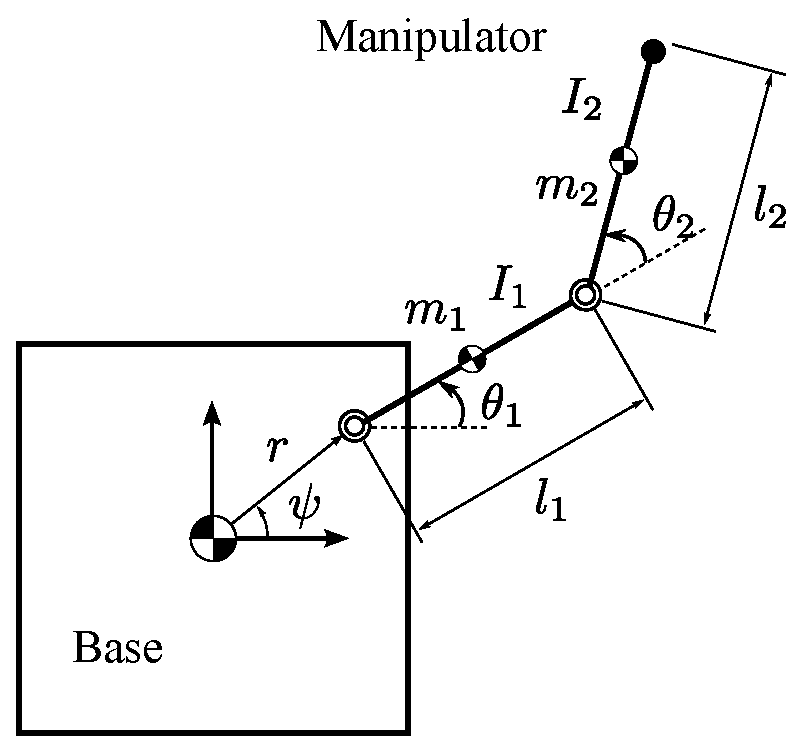
\includegraphics[width=1.0\linewidth]{fig/chapter3/planar/FF2RModel.eps}
  \end{minipage}
  \hspace{4mm}
  \begin{minipage}[t]{0.30\linewidth}
    \centering
    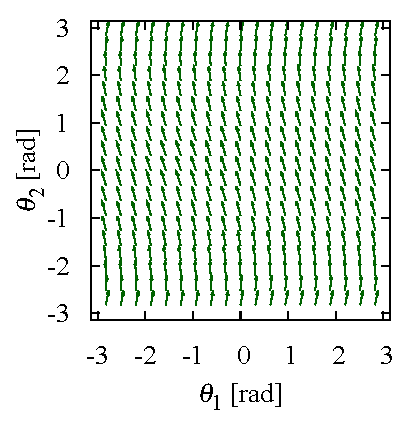
\includegraphics[width=1.0\linewidth]{fig/chapter3/planar/vectorField.eps}
  \end{minipage}
  \caption{A planar two-DoF space manipulator model with $m_{i} = 100\unit{kg}$,
  $l_{i} = 1.0\unit{m}$ ($i = 1, 2$); the base mass is $m_{b} = 1000\unit{kg}$.
  The vector field is obtain with $r = 0\unit{m}$.}
  \label{fig:FF2R}
\end{figure}
% ---------------------------------------------------------------------
%
Existing results from reactionless motion control have been reported in the Introduction. 
There are, however, some  characteristics of reactionless motion that have not been mentioned so far.

Consider first a simple planar two-DoF manipulator on a satellite base, as shown in \fig{FF2R}.
This model is the simplest one with the capability of reactionless motion generation.
Reactionless motion with this model can be represented as follows:
%
% ---------------------------------------------------------------------
\begin{align}
  \thd = b\bm{n}(\th)\label{eq:RNSSYST}
\end{align}
% ---------------------------------------------------------------------
%
where $\bm{n}(\th)\R{2}$ is the only generic null-space vector in the kernel 
of the coupling inertia matrix, and $b$ is an arbitrary scalar dimensioned as joint velocity.
$\bm{n}(\th)$ can be uniquely obtained through appropriate methods,
i.e.\ Singular Value Decomposition (SVD) or the co-factor method.
We assume that $\bm{n}(\th)$ is already normalized,
and $b$ is a time-independent constant scalar, for the sake of simplicity.
Hence, \eq{RNSSYST} can be regarded as an autonomous nonlinear system.
The right hand side in \eq{RNSSYST} defines the vector field of reactionless motion
in joint space.

%We examine the properties of reactionless motion with the above vector field.
For the sake of simplicity, we assume that the manipulator is attached at the CoM of the base.
The mass and inertia moment of the base are $m_{b} = 1000\unit{kg}$, ${I}_{b} = 667\unit{kgm^{2}}$;
the length, mass and inertia moments of the links are $l_{i} = 1.0\unit{m}$,
$m_{i} = 100\unit{kg}$ and ${I}_{i} = 8.33\unit{kgm^{2}}$ ($i = 1,2$), respectively.
The resultant vector field is depicted in \fig{FF2R}. 
Because the manipulator is attached symmetrically,
the vector field has rotational symmetry w.r.t.\ Joint 1.
From the vector field, an important property becomes apparent:  reactionless motion is predominantly 
composed of Joint 2 motion. 
Because reactionless motion  conserves  angular momentum at zero (or at a constant),
motion in the joints that induce a large angular momentum cannot variate significantly.
With this model, the angular momentum induced by Joint 1 motion must be larger than
that of Joint 2  due to the large inertia moment and the long moment arm. 
As a result, the above mentioned behavior is observed.

%%%%%%%%%%%%%%%%%%%%%%%%%%%%%%%%%%%%%%%%%%%%%%%
\subsection{Fixed point and bifurcation}
\label{sec:ANALYSIS_FIXED}
%%%%%%%%%%%%%%%%%%%%%%%%%%%%%%%%%%%%%%%%%%%%%%%
In the above example, the system does not have any fixed points.
It turns out, however, that the variation of the manipulator attachment position
induces such points and moreover, a bifurcation can be observed.
The attachment position is made variable according to:
%
% ---------------------------------------------------------------------
\begin{align}
  \begin{bmatrix}
    x_{a}\\
    y_{a}
  \end{bmatrix}
  =
  r
  \begin{bmatrix}
    \cos\psi\\
    \sin\psi
  \end{bmatrix}
\end{align}
% ---------------------------------------------------------------------
%
where %$(\circ)_{a}$ is the coordinate of the attachment position,
$r$ is the distance between the attachment position and the base CoM,
and $\psi$ is the angle as shown in \fig{FF2R}.
Among these parameters, $r$ plays an important role as a \textit{bifurcation parameter} in this system.
Note that we can assume $\psi = 0$ because this parameter does not influence the topological structure
of the system due to the existing rotational symmetry. Hence, it is sufficient to variate 
the attachment position along the $x$-axis of the base frame.

%
% --------------------------------------------------------------------
\begin{figure}[t]
  \centering
  \begin{minipage}[t]{0.30\linewidth}
    \centering
    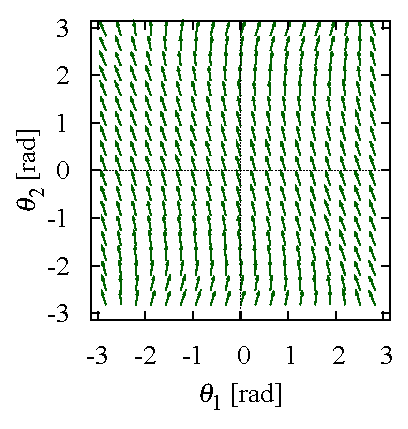
\includegraphics[width=1.0\linewidth]{fig/chapter3/planar/0.5.eps}
    \hspace{2mm}
  \end{minipage}
  \begin{minipage}[t]{0.30\linewidth}
    \centering
    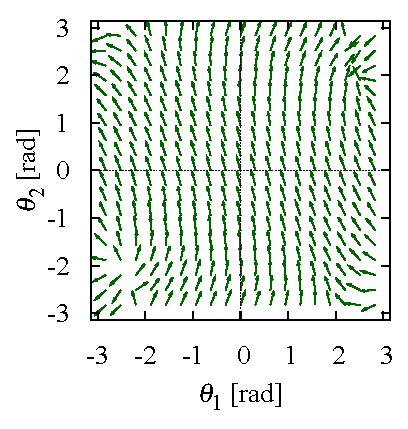
\includegraphics[width=1.0\linewidth]{fig/chapter3/planar/0.945.eps}
    \hspace{2mm}
  \end{minipage}
  \begin{minipage}[t]{0.30\linewidth}
    \centering
    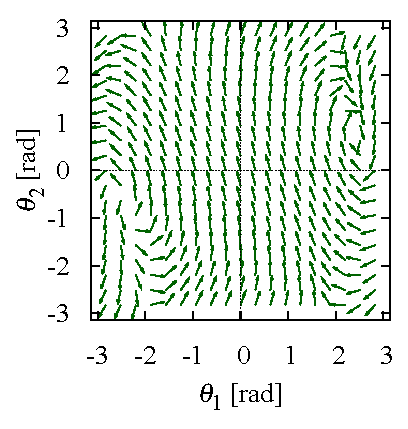
\includegraphics[width=1.0\linewidth]{fig/chapter3/planar/1.5.eps}
    \hspace{2mm}
  \end{minipage}\\
  \vspace{-3mm}
  \begin{minipage}[t]{0.30\linewidth}
    \centering
    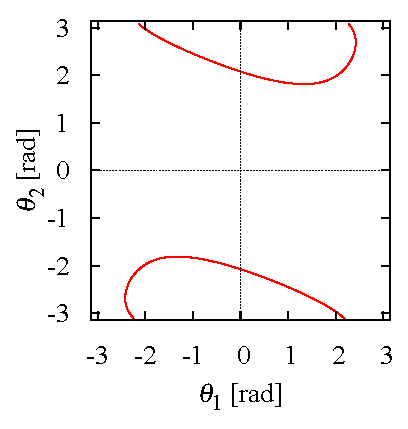
\includegraphics[width=1.0\linewidth]{fig/chapter3/planar/0.5_nullclines.eps}
    \footnotesize\par{(a)}
    \hspace{2mm}
  \end{minipage}
  \begin{minipage}[t]{0.30\linewidth}
    \centering
    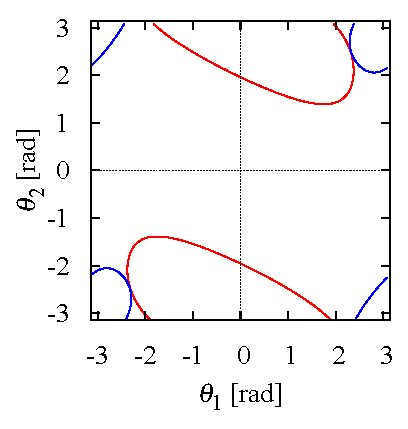
\includegraphics[width=1.0\linewidth]{fig/chapter3/planar/0.945_nullclines.eps}
    \footnotesize\par{(b)}
    \hspace{2mm}
  \end{minipage}
  \begin{minipage}[t]{0.30\linewidth}
    \centering
    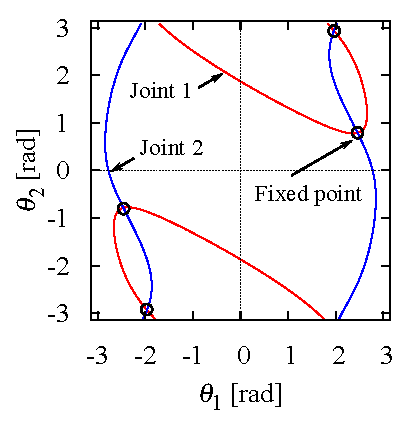
\includegraphics[width=1.0\linewidth]{fig/chapter3/planar/1.5_nullclines.eps}
    \footnotesize\par{(c)}
    \hspace{2mm}
  \end{minipage}
  \caption{The vector field and nullclines for each joint direction when $r$ variates as: 
    (a) $r = 0.5\unit{m}$, (b) $r = 0.945\unit{m}$ and (c) $r = 1.5\unit{m}$.}
    \label{fig:BIF_VEC}
\end{figure}
% --------------------------------------------------------------------
%
In \fig{BIF_VEC},  the vector field and nullclines for  several values of $r$ are shown.
In the figures, the upper part represents the vector field and
the lower part depicts nullclines for each joint direction:
the lines in red are for Joint 1, those  in blue are  for Joint 2. 
When $r = 0.5\unit{m}$, we can see that there is no fixed point,
because the motion of Joint 2 never stops at any point in joint space.
On the other hand, the occurrence of a bifurcation can be observed when 
$r \approx 0.945\unit{m}$.
Then, two fixed points are created at the intersection points of the two nullclines.
Further increase of the bifurcation parameter ($r = 1.5\unit{m}$) 
leads to separation of the created fixed points. 
Finally, when $r \rightarrow \infty$, two of the fixed points converge to
$\theta_{2} \rightarrow 0\unit{rad}$ and
the rest  to $\theta_{2} \rightarrow \pm\pi\unit{rad}$.

%%%%%%%%%%%%%%%%%%%%%%%%%%%%%%%%%%%%%%%%%%%%%%%%%%%%%%%%%%%%%%%%
\subsection{Rank deficiency of the coupling inertia matrix}
\label{sec:ANALYSIS_SING}
%%%%%%%%%%%%%%%%%%%%%%%%%%%%%%%%%%%%%%%%%%%%%%%%%%%%%%%%%%%%%%%%
In above discussion, we clarified the existence of fixed points with regard to reactionless motion.
This phenomenon is related to the rank deficiency of the coupling inertia matrix.
In contrast to kinematic singularities, the singularities of the coupling inertia matrix have 
not been discussed, so far. We provide some insight with the planar model mentioned above.

%
% ---------------------------------------------------------------------
\begin{figure}[t]
  \centering
  \begin{minipage}[t]{0.42\linewidth}
    \centering
    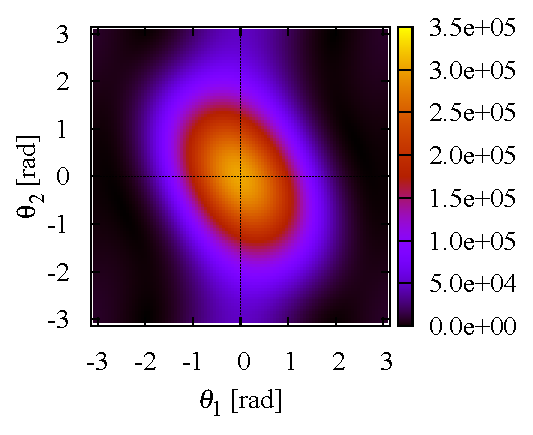
\includegraphics[width=1.0\linewidth]{fig/chapter3/planar/determinant.eps}
    \footnotesize\par{(a)}
  \end{minipage}
  \hspace{1mm}
  \begin{minipage}[t]{0.38\linewidth}
    \centering
    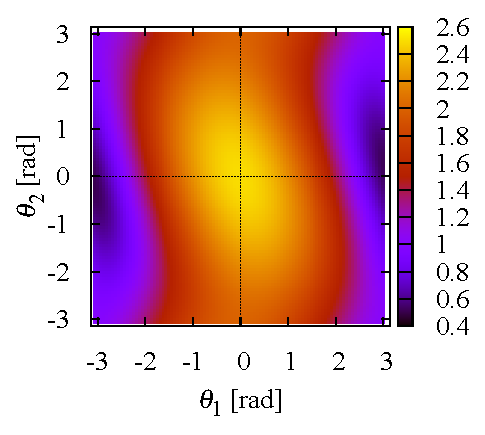
\includegraphics[width=1.0\linewidth]{fig/chapter3/planar/com.eps}
    \footnotesize\par{(b)}
  \end{minipage}
  \caption{This figure shows the determinant of $(\bm{M}_{\omega m}\tbm{M}_{\omega m}^{T})$ and
  the distance between the manipulator CoM and the base one as color map:
  (a) $\mathrm{det}(\tbm{M}_{\omega m}\tbm{M}_{\omega m})$ and (b) the distance between the manipulator CoM and the base one.}
  \label{fig:DET_FF2R}
\end{figure}
% ---------------------------------------------------------------------
%
Determinant $\det (\tbm{M}_{\omega m}\tbm{M}_{\omega m}^{T})$
for  $r = 1.5\unit{m}$ is shown as a colored map in \fig{DET_FF2R}~(a).
The determinant takes large values at the bright areas, 
while the most dark area represents the singularities.
It is apparent that the determinant takes its maximum value at $\th = \bm 0$.
This is an extended-arm configuration s.t.\ the manipulator CoM is located farthest away 
from the base CoM. Note that determinant $\det(\tbm{M}_{\omega m}\tbm{M}_{\omega m}^{T})$ can be 
related to the distance between the two CoMs as shown in
%, which is depicted on the joint space plane in  
\fig{DET_FF2R}~(b). Comparing the two plots in \fig{DET_FF2R}, it can be seen that the determinant
takes large values whenever the distance is relatively large. Large CoM distance yields 
large  moment of  momentum and hence, large magnitude of the coupling angular momentum.  
Furthermore, note that there is no fixed point within the area where the distance is large.
In the case of a spatial model, the directions  of the joint axes play an 
important role in addition to the above qualitative characteristics. 

%%%%%%%%%%%%%%%%%%%%%
\section{Summary}
%%%%%%%%%%%%%%%%%%%%%
In this chapter,
we described some characters of reactionless motion with a planar model.
From a qualitative analysis,
we found out that the manipulator attachment position plays an important role
in terms of bifurcation.
Then, through vector field,
we confirmed that the fixed points of reactionless motion are generated,
increasing the length between the manipulator attachment position and the base CoM.







%**********************************************************************
%
%
%%% Local Variables:
%%% mode: latex
%%% TeX-master: "./main"
%%% End:

\chapter{Proposal of Reactionless Tasks}
\label{cha:PROPOSAL}
% Abstract for this chapter
%
%**********************************************************************
In this chapter,
we discuss motion tasks suitable for execution under reactionless motion control,
with a seven-DoF redundant manipulator.
First, we will show that the reactionless motion of the model consists of the predominant wrist and elbow motion.
Based on these motions,
we propose the following three tasks \cite{Sone2015}:
(i) inspection task using a hand-held camera,
(ii) point-to-point position control,
(iii) deployment task from a stowed configuration.
The performance of these tasks are verified via numerical simulation.

%%%%%%%%%%%%%%%%%%%%%%%%%%%%%%%%
\section{Manipulator model}
\label{sec:MODEL}
%%%%%%%%%%%%%%%%%%%%%%%%%%%%%%%%
%%%%%%%%%%%%%%%%%%%%%%%%%%%%%%%%
\subsection{Model description}
%%%%%%%%%%%%%%%%%%%%%%%%%%%%%%%%

%
% ---------------------------------------------------------------------
\begin{figure}[t]
  \centering
  \begin{minipage}{0.25\linewidth}
    \centering
    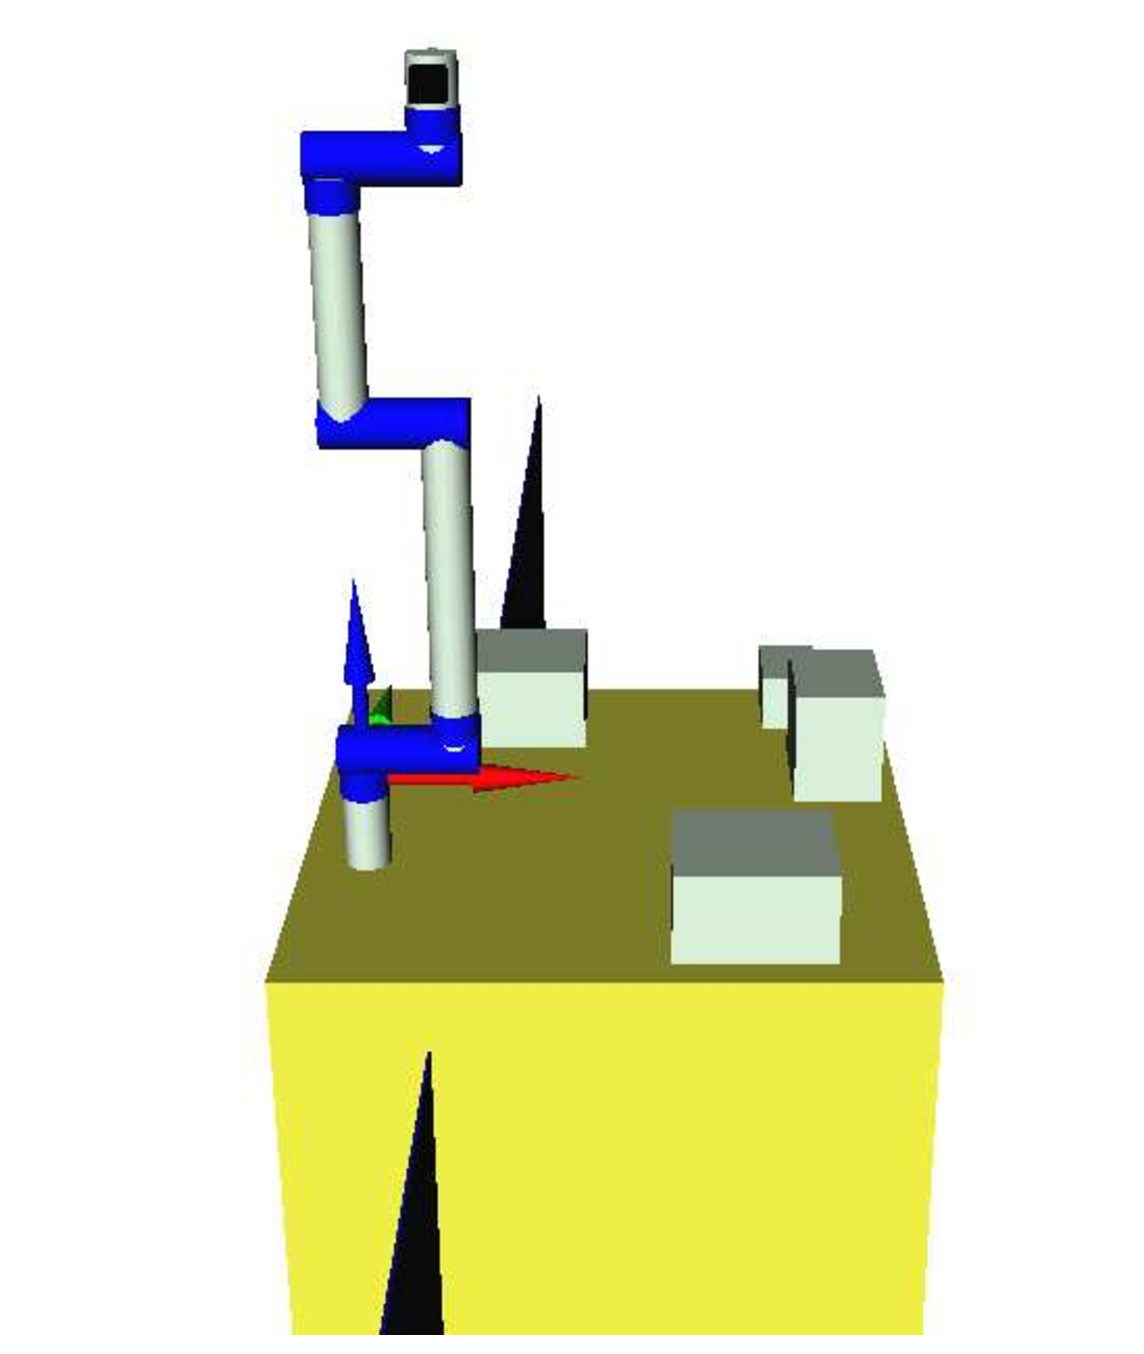
\includegraphics[width=1.0\linewidth]{fig/chapter4/init.eps}
  \end{minipage}
  \begin{minipage}{0.65\linewidth}
    \centering
    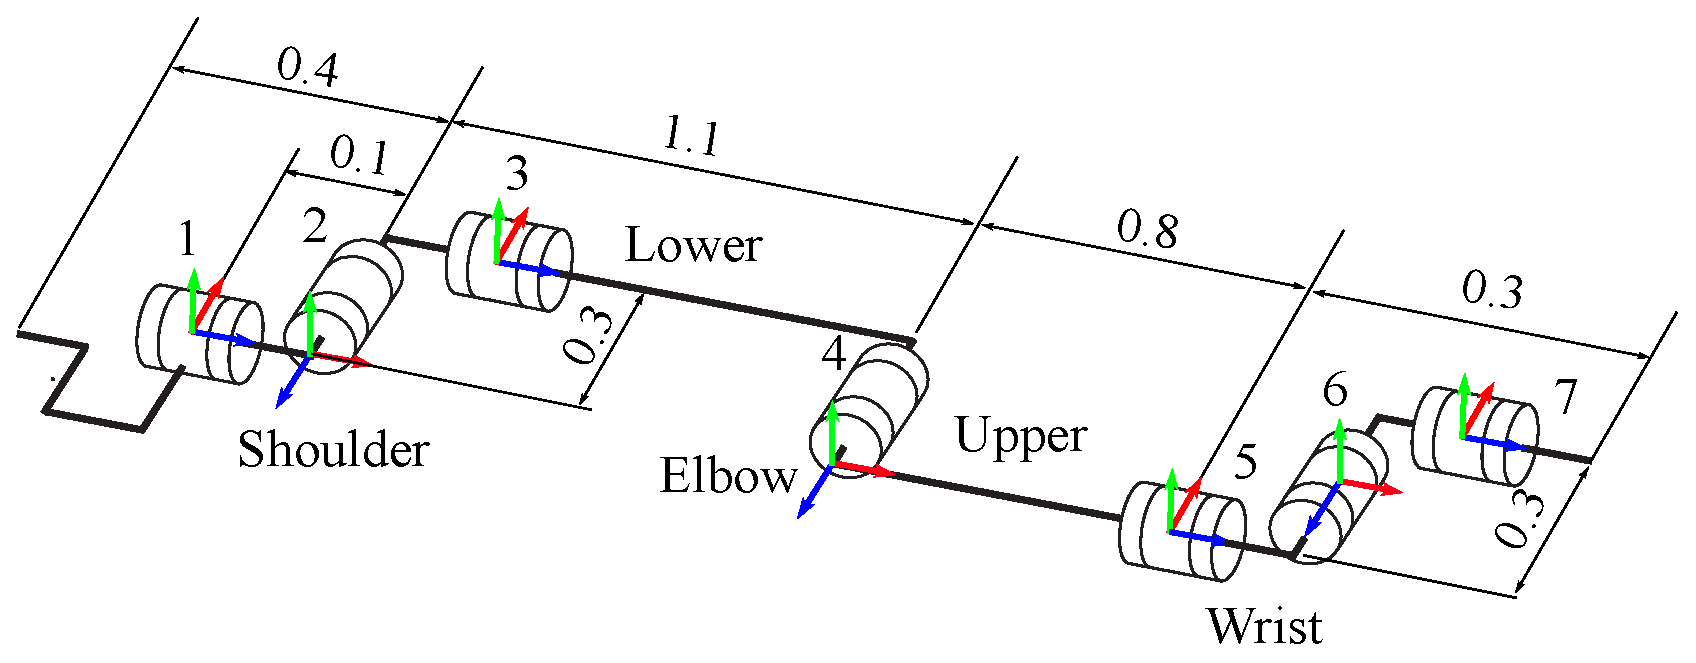
\includegraphics[width=1.0\linewidth]{fig/chapter4/typeA_7R.eps}    
  \end{minipage}
  \caption{Our manipulator model with seven-DoF mechanism at the initial configuration ($\theta_{i} = 0\unit{rad},~\forall\theta_{i}$).}
  \label{fig:MODEL}
\end{figure}
% ---------------------------------------------------------------------
%
We consider a free-flying space robot model consisting of a satellite base,
and a serial-link seven-DoF kinematically redundant manipulator.
The manipulator is characterized by a kinematic chain with a distinctive lower/upper arm
subchain, including a rotational ``elbow'' joint, a ``shoulder'' and a ``wrist'' joint, all of them  
with offsets. The kinematic structure and simulation model are displayed in \fig{MODEL}.
The manipulator attachment position is determined from the ETS-VII design, at $[-0.79~-0.29~1.0]^{T}\unit{m}$
with respect to the base CoM coordinate frame \cite{Yoshida2003}.
The dynamic model parameters are shown in \tab{parameter}.
%
% ---------------------------------------------------------------------
\begin{table}[t]
  \centering
  \caption{Dynamic model parameters}
  \begin{tabular}[h]{c||c|c|c|c}\hline\hline
    & Mass [kg]&
    \multicolumn{3}{ c }{Inertia moment [$\mathrm{kgm^{2}}$]}\\\hline
    $i$ & $m_{i}$&  $I_{xi}$ & $I_{yi}$ & $I_{zi}$ \\\hline\hline
    1 & 30.0 & 0.0671 & 0.0671& 0.0851\\\hline
    2 & 30.0 & 0.0843& 0.267 & 0.267\\\hline
    3 & 45.0 & 3.81 & 3.81& 0.127 \\\hline
    4 & 40.0 & 0.113& 2.19 & 2.19\\\hline
    5 & 20.0 & 0.213 & 0.213 & 0.0250\\\hline
    6 & 20.0 & 0.0250 & 0.0292 & 0.0292\\\hline
    7 & 25.0 & 0.0990& 0.0990 & 0.0313\\\hline
  \end{tabular}
  \label{tab:parameter}
\end{table}
% ---------------------------------------------------------------------
%
%%%%%%%%%%%%%%%%%%%%%%%%%%%%%%%%%%%%%%%%%%%%%%%%%%
\subsection{Reactionless motion representation}
%%%%%%%%%%%%%%%%%%%%%%%%%%%%%%%%%%%%%%%%%%%%%%%%%%

Before proceeding with the analysis of the reactionless motion task,
we have to identify the reactionless motion capability with the manipulator model.
First, note that the DoF of reactionless motion is four, 
which is obtained as the difference between the number of joints (seven) 
and the base attitude variables (three).
The following discussion provides a useful representation of the four-DoF reactionless motion.

For the analysis, we divide the kinematic chain into two subchains: 
the positioning subchain comprising  joints 1 through 4, and the wrist subchain 
comprising the rest of the joints. Then, we focus on the amplitude of the angular momentum 
produced by each of the two subchains. Because of the serial-link structure, the  wrist subchain is 
characterized with relatively small mass and length of the moment arm. 

Dividing joint velocity into the positioning and wrist subchain related terms,
we can rewrite the reactionless constraint as follows:
%
% ---------------------------------------------------------------------
\begin{align}
  \tbm{M}_{P\omega m}\thd_{P} + \tbm{M}_{W\omega m}\thd_{W} = \bm{0}
\end{align}
% ---------------------------------------------------------------------
%
where $\thd = [\thd_{P}~\thd_{W}]$,
$\tbm{M}_{\omega m} = [\tbm{M}_{P\omega m}~\tbm{M}_{W\omega m}]$;
$(\circ)_{P}$ and $(\circ)_{W}$ represent the quantities related to the positioning and wrist subchains.
In the above equation, the first term is the partial angular momentum produced by the positioning subchain;
the second term is stemming from the wrist subchain.

Next, we focus on the amplitude of these angular momentum.
Because of the small mass and the length of moment arm of the wrist subchain,
the angular momentum produced by the motion of the wrist subchain will be far smaller than that
obtained from the positioning subchain. Therefore, we can assume that the positioning subchain 
can compensate the base disturbance induced by the wrist subchain motion, completely.
This implies one particular reactionless motion patterns, characterized with ``unconstrained'' 
wrist motion plus small compensating variations in the positioning subchain, as shown in \fig{motion}~(a).
This motion is a three-DoF reactionless motion and is referred to  as
the {\sl predominant wrist motion}, hereafter.
This motion can be obtained as follows:
%
% ---------------------------------------------------------------------
\begin{align}
  \thd = \bmat{\bm{B}(\th) \\ \bm{E}}\thd_{W}\label{eq:RL_POS}
\end{align}
% ---------------------------------------------------------------------
%
where $\bm{B} = -\tbm{M}_{P\omega m}^{+}\tbm{M}_{W\omega m}\R{4 \times 3}$
is a linear map from the wrist subchain motion to the
positioning subchain motion ensuring the reactionless constraint.

%
% ---------------------------------------------------------------------
\begin{figure}[t]
  \centering
  \begin{minipage}[h]{0.4\linewidth}
    \centering
    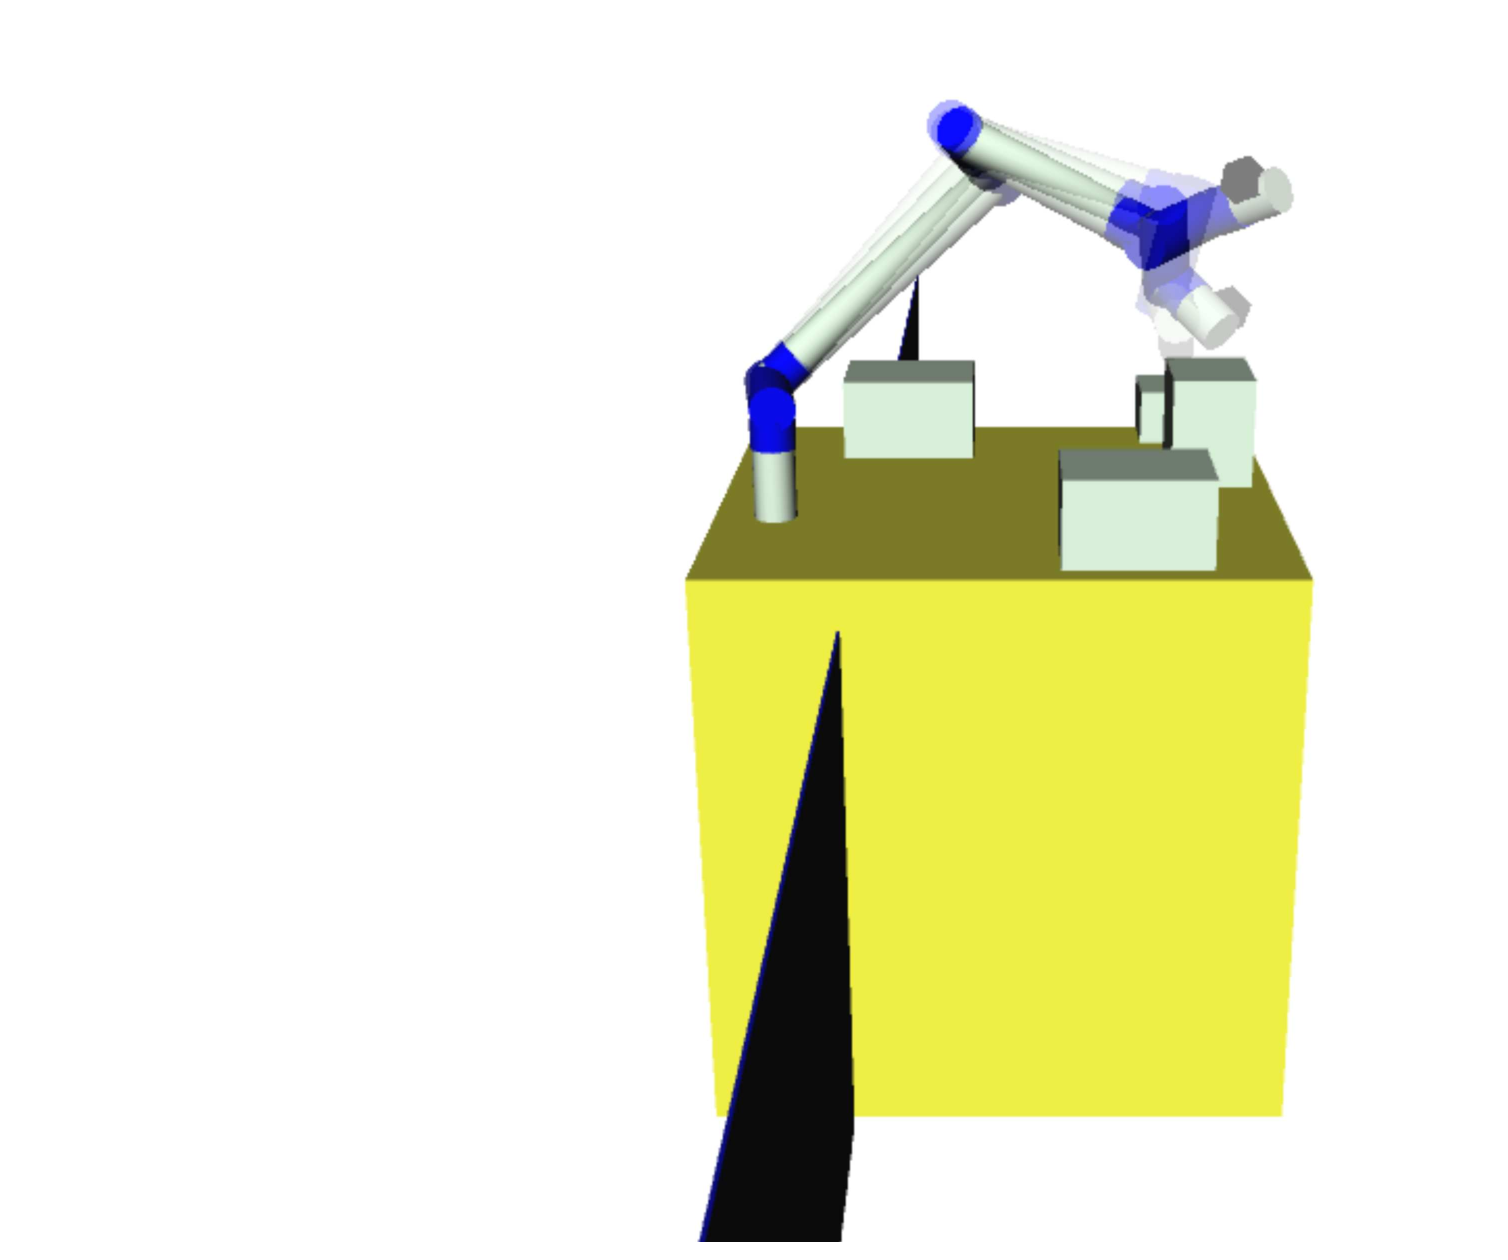
\includegraphics[width=1.0\linewidth]{fig/chapter4/spatial/WS.eps}
    \footnotesize\par{(a)}
  \end{minipage}
  \begin{minipage}[h]{0.4\linewidth}
    \centering
    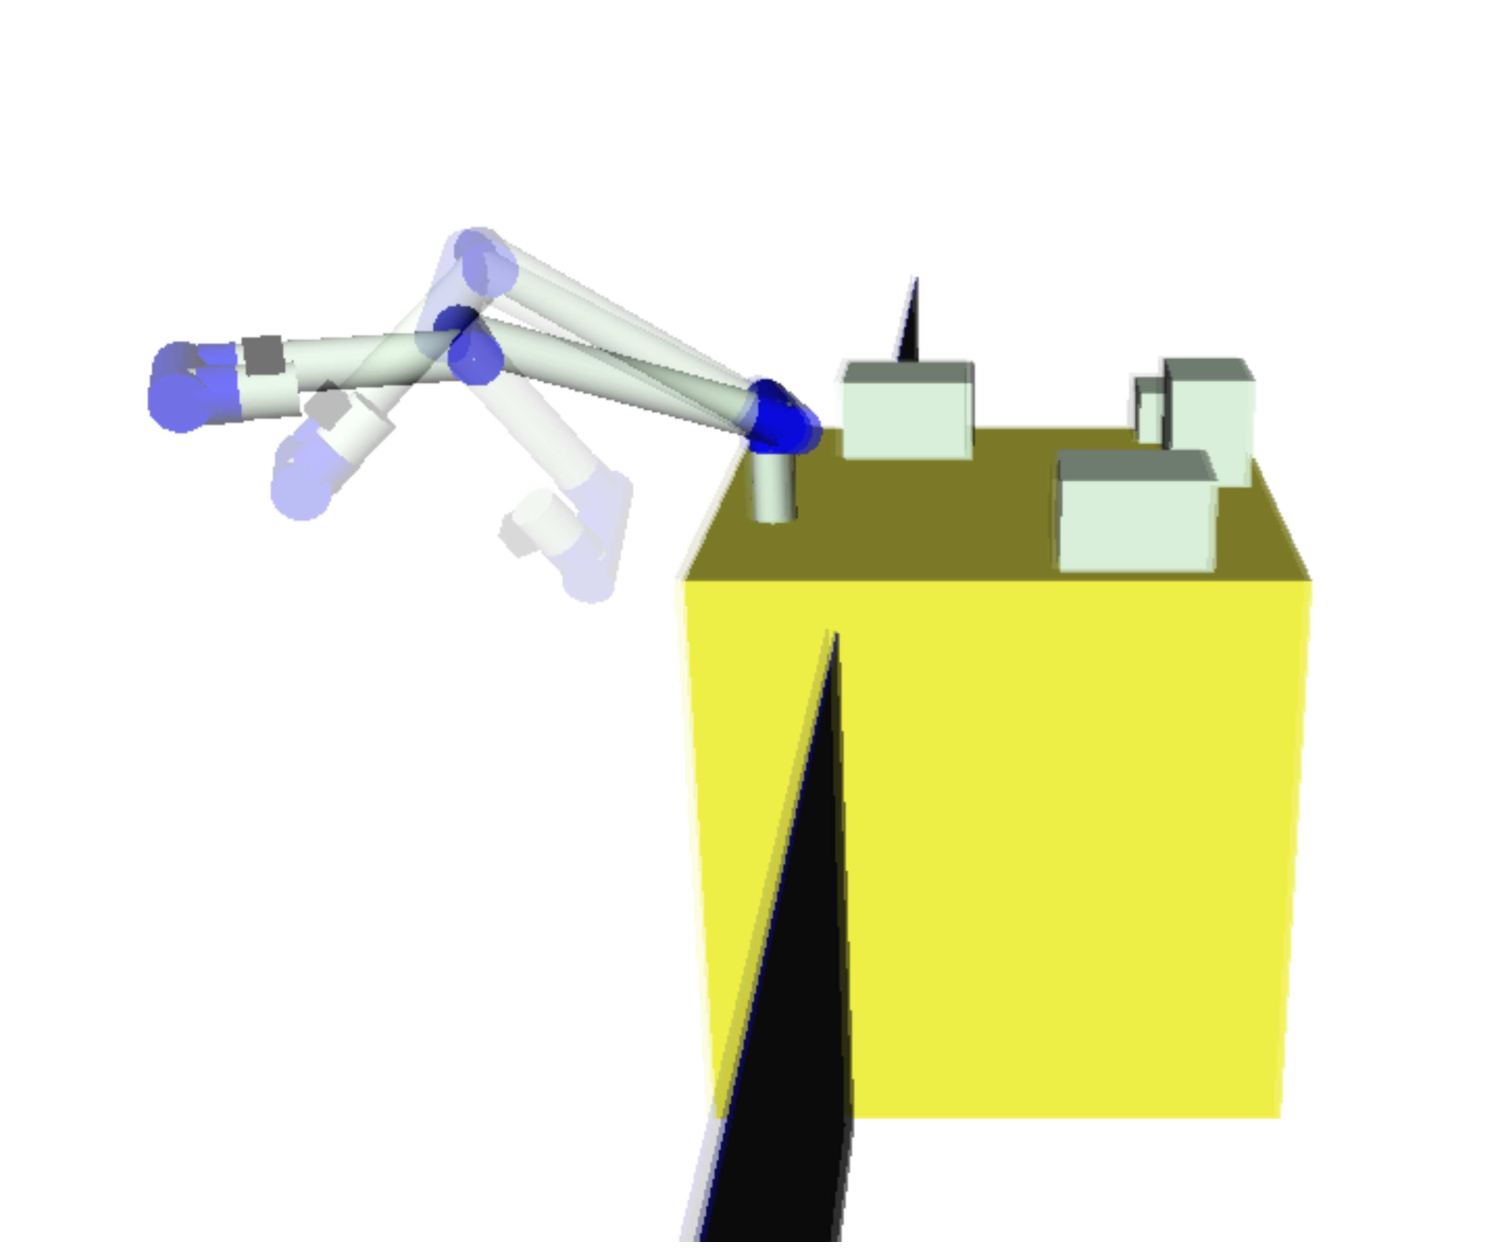
\includegraphics[width=1.0\linewidth]{fig/chapter4/spatial/PS.eps}
    \footnotesize\par{(b)}
  \end{minipage}
  \caption{Reactionless motion of the manipulator model: (a) the predominant wrist motion and (b) the elbow folding motion.}
  \label{fig:motion}
\end{figure}
% ---------------------------------------------------------------------
%

The remaining one-DoF reactionless motion is uniquely determined from the null-space vector
of the coupling inertia submatrix that is related to the positioning subchain $\tilde{\bm{M}}_{\omega mP}$.
%
% ---------------------------------------------------------------------
\begin{align}
  \thd = b \bmat{\bm{n}(\th) \\ \bm{0}}
\end{align}
% ---------------------------------------------------------------------
%
where $b$ is an arbitrary scalar.
From the angular momentum conservation, we can assume that motions in Joints 1 and 2 will be
relatively small for  the above two reactionless motion patterns.
Hence, this motion approximately consists of the elbow folding/unfolding motion as shown in \fig{motion}~(b).

Since these two patterns are  orthogonal, their superposition will represent all possible reactionless
motions for the given manipulator model, as follows:
%
% ---------------------------------------------------------------------
\begin{align}
  \thd &= \bmat{\bm{B}(\th) \\ \bm{E}}\thd_{W} + b \bmat{\bm{n}(\th) \\ \bm{0}}
\end{align}
% ---------------------------------------------------------------------
%
From the above analysis,
we can then arrive at the following conclusion:
because the end-effector position largely depends on the motion in the positioning subchain,
it follows that under reactionless motion, the positioning DoF of end-effector will be 
approximately one. This feature results only from the specific kinematic structure of the
positioning subchain, comprising two upper/lower arm links (i.e.\ it is similar to the 
two-link planar example discussed previously).
Therefore, we will henceforth focus on reactionless end-effector orientation control
with the predominant wrist motion and reactionless manipulator configuration control.
This makes our research different from previous studies.

Based on the two type of reactionless motions,
we propose the following three tasks for reactionless motion:
(i) inspection task using a hand-held camera,
(ii) point-to-point positioning task and
(iii) deployment task from a stowed configuration.
First, we describe the inspection task in what follows.

%%%%%%%%%%%%%%%%%%%%%%%%%%%%%%%%%%%%%%%%%%%%%%%%%%%%%%%%%%%
\section{Inspection task using a hand-held camera}
\label{sec:INSPECTION}
%%%%%%%%%%%%%%%%%%%%%%%%%%%%%%%%%%%%%%%%%%%%%%%%%%%%%%%%%%%

%
% ---------------------------------------------------------------------
\begin{figure}[t]
  \centering
  \begin{minipage}[h]{0.495\linewidth}
    \centering
    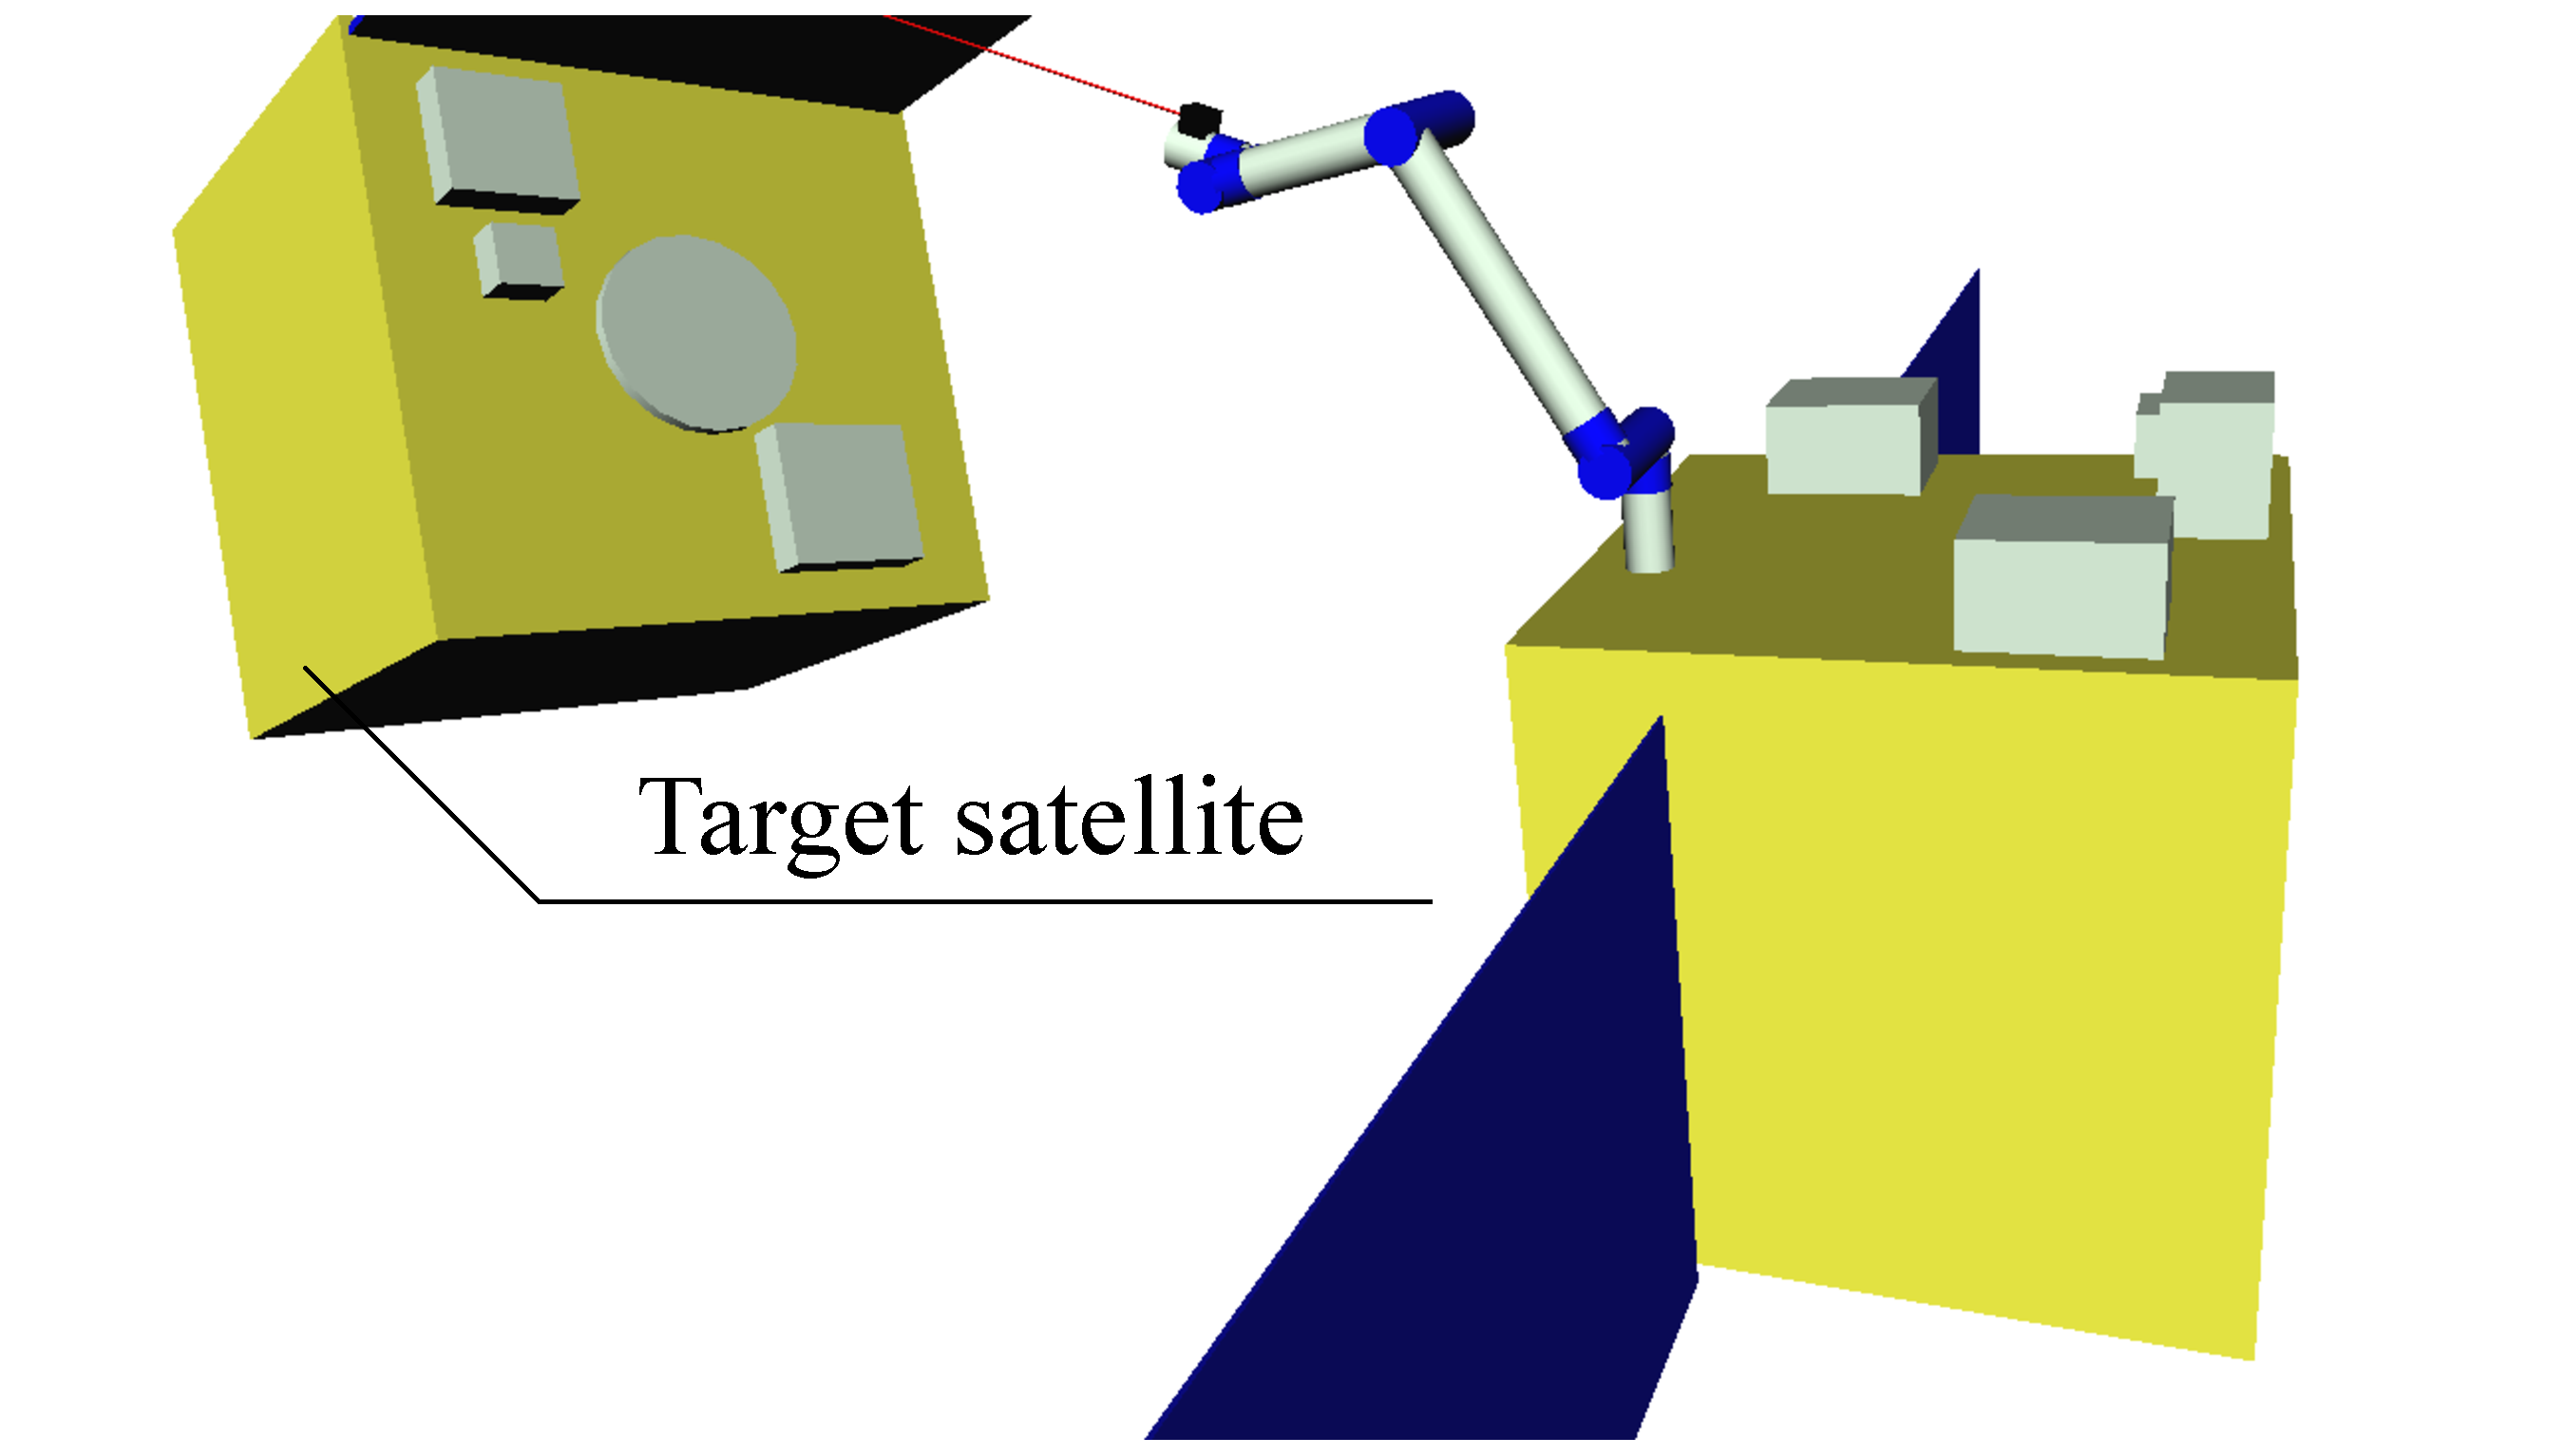
\includegraphics[width=1.0\linewidth]{fig/chapter4/inspection/observation.eps}
    \footnotesize\par{(a)}
  \end{minipage}
  \begin{minipage}[h]{0.495\linewidth}
    \centering
    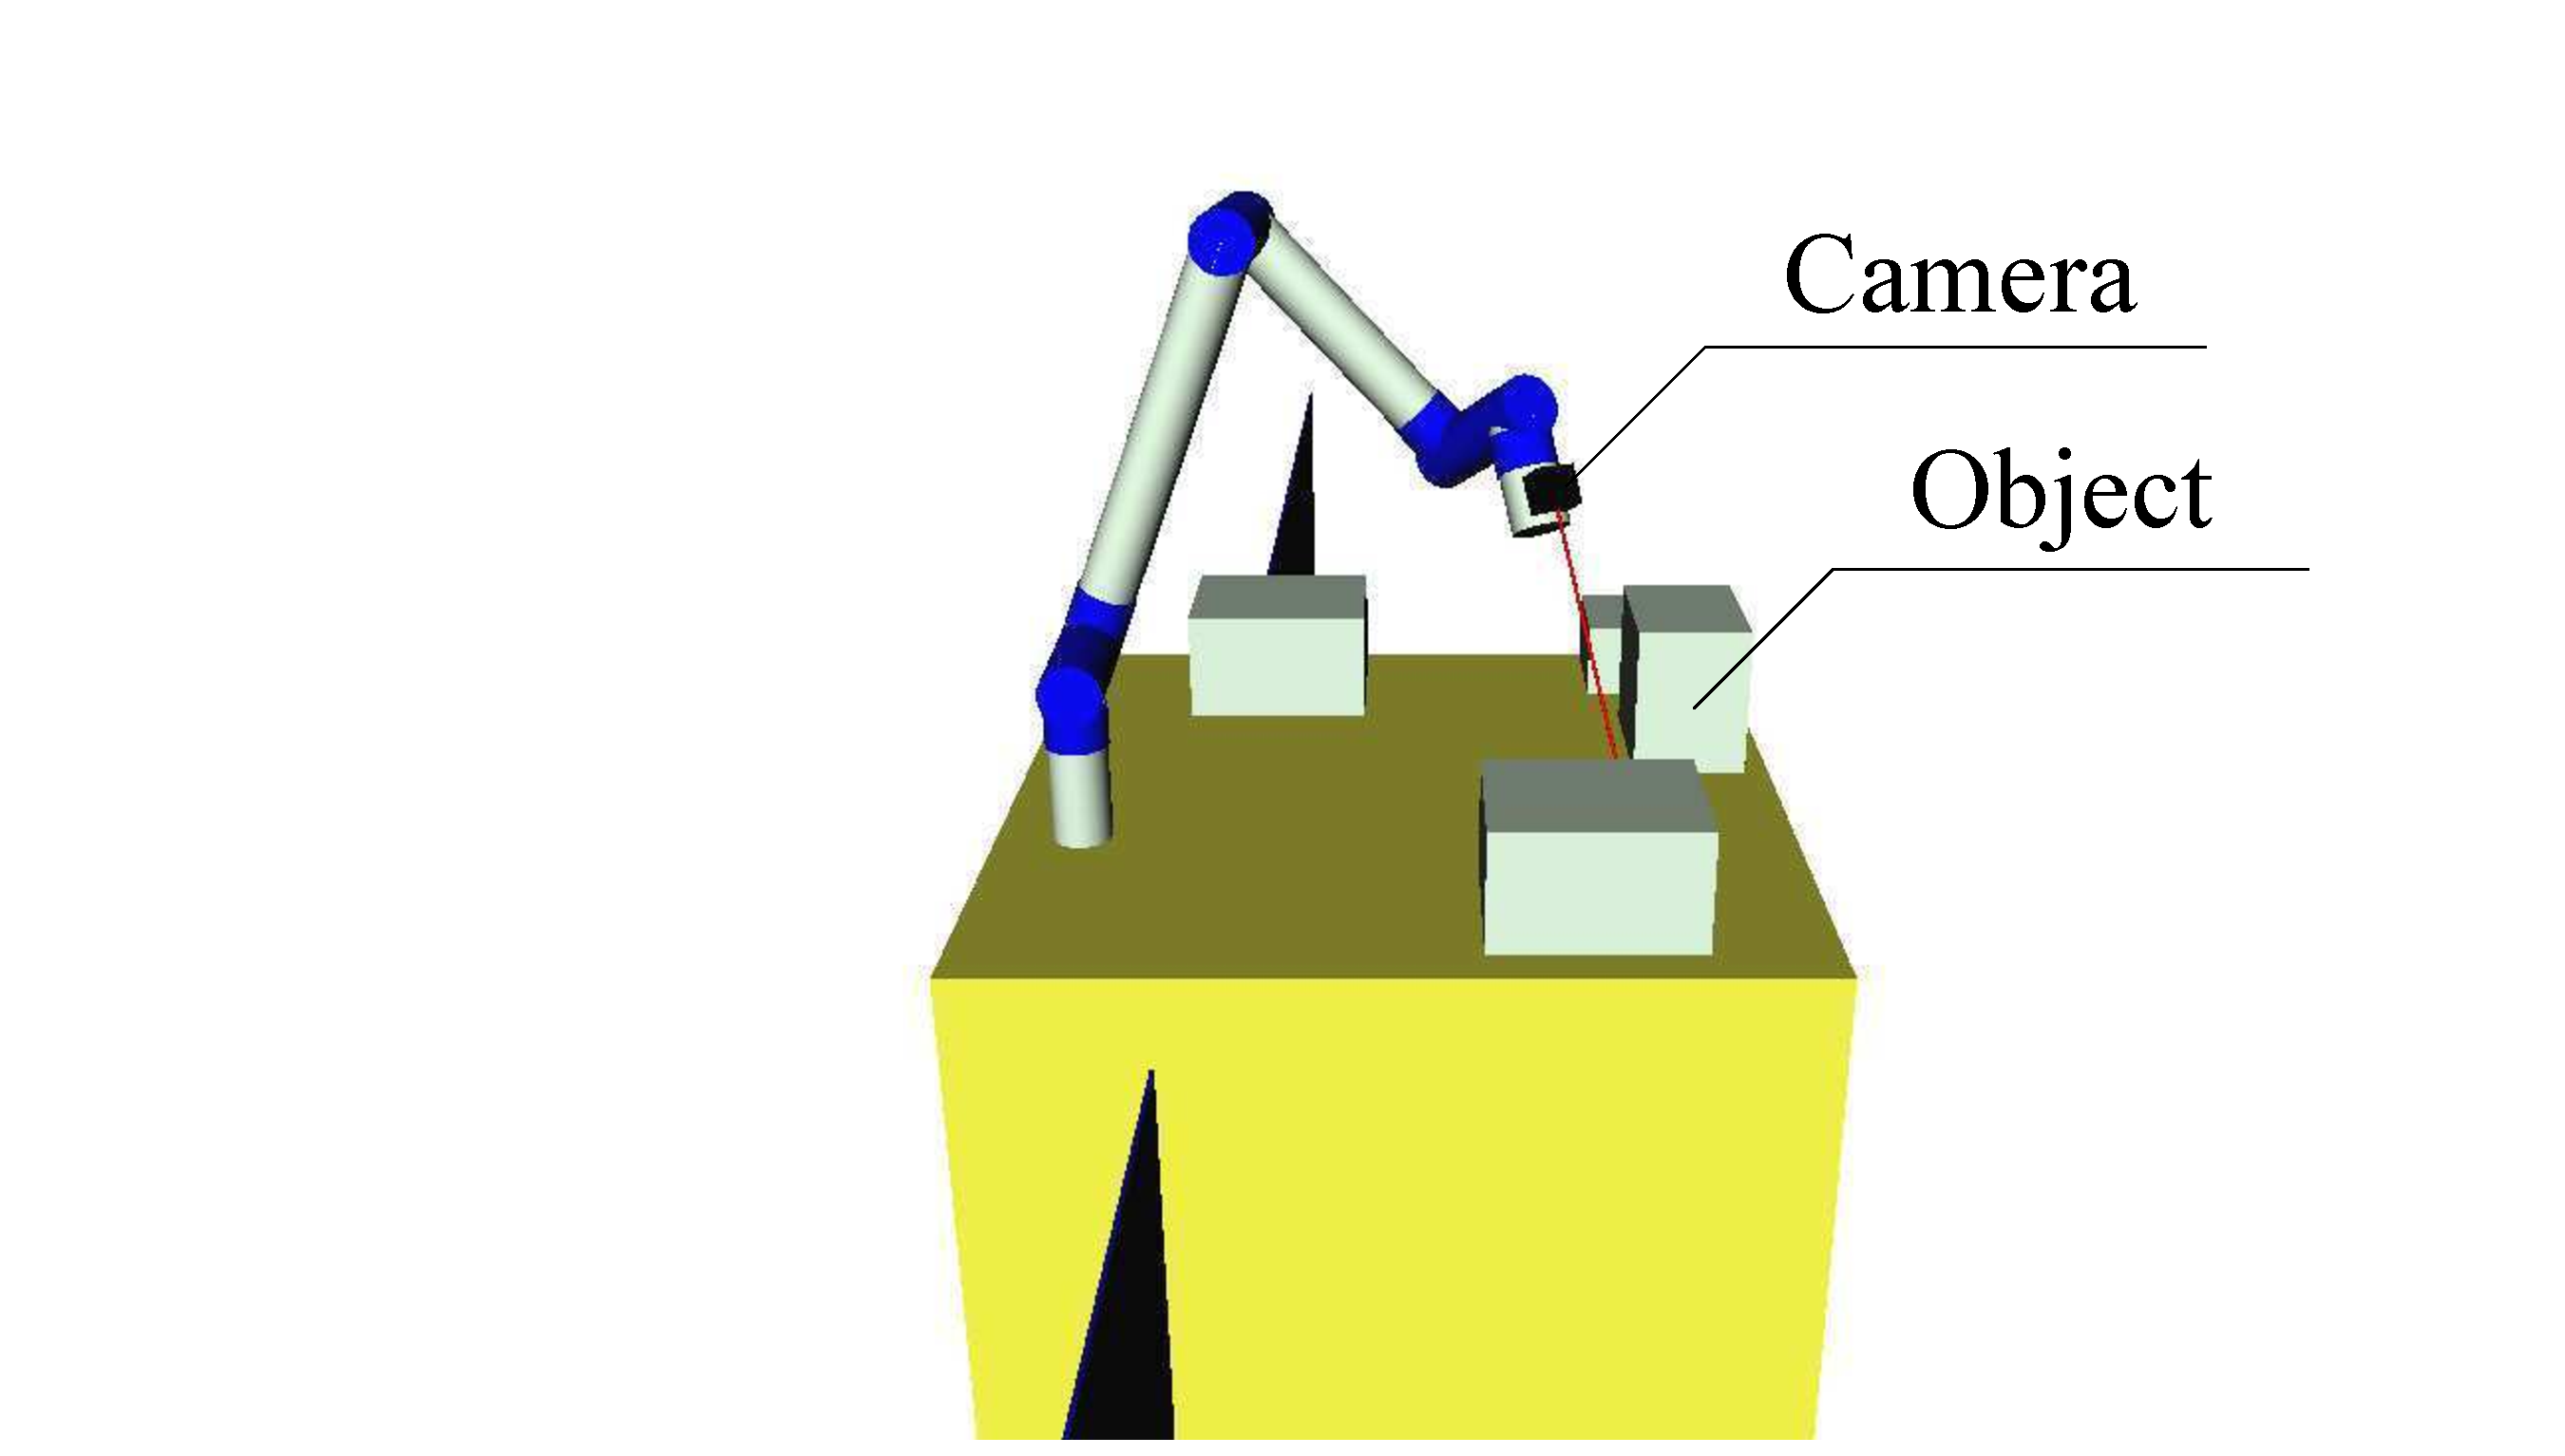
\includegraphics[width=1.0\linewidth]{fig/chapter4/inspection/inspection.eps}
    \footnotesize\par{(b)}
  \end{minipage}
  \caption{Inspection task using the hand-held camera: 
    (a) target satellite to be refueled of captured and (b) own-satellite attached devices.}
  \label{fig:ins}
\end{figure}
% ---------------------------------------------------------------------
%
One frequently appearing task for free-floating space robots is inspection with a hand-held camera 
of devices mounted on the own satellite base or on the satellite to be serviced, 
as shown in \fig{ins}.
Such task was also performed within the ETS-VII mission \cite{Oda1997} but without using 
reactionless control. For camera inspection, once the arm is positioned appropriately,
the camera view angle for inspection is changed by rotating the wrist.
This task is  expected to be performed multiple times during a number of missions,
such as construction, maintenance, debris removal and so on.
Hence, this task is a good candidate for execution under reactionless motion control
for improved work efficiency.

The following three control subtasks are considered necessary to accomplish  camera inspection.
%
% ---------------------------------------------------------------------
\begin{enumerate}
\item Reactionless constraint of the base attitude (three-DoF).
\item Orientation control of the wrist (three-DoF).
\item Stabilization of the wrist position.
\end{enumerate}
% ---------------------------------------------------------------------
%
The first control subtask ensures reactionless motion. The second one is essential for camera 
inspection. The third control subtask is necessary to avoid a large deflection of the wrist from the 
initial position, since there is no position control subtask.
The above subtasks will be simultaneously realized through  consecutive null-space projections 
\cite{Konstantinov1981, Nakamura1981}, known also as the task-of-priority approach \cite{Nakamura1987}.
Priorities are assigned among the tasks according to their relative importance.
A higher-priority task can then be accomplished without being disturbed  from the lower-priority tasks.
This is ensured by projecting lower-priority tasks onto the common null-space of 
all higher-priority tasks.


%%%%%%%%%%%%%%%%%%%%%%%%%%%%%%%%%%
\subsection{Control command}
\label{sec:CONTROLLER}
%%%%%%%%%%%%%%%%%%%%%%%%%%%%%%%%%%
The priorities are assigned as follows.  The reactionless constraint is the highest-priority subtask,
wrist orientation control is the second-priority one and wrist position stabilization is the 
lowest-priority subtask. The control command for the joint velocity  
can then be obtained as follows:
%
% ---------------------------------------------------------------------
\begin{align}
  \thd^{ref} = \bar{\bm{J}}_{\omega_{e}}^{+}\bm{\omega}_{e}^{ref} + k_{g}\bm{P}\bm{J}_{v_{w}}^{T}\Delta\bm{p}_{w}
  \label{eq:REF}
\end{align}
% ---------------------------------------------------------------------
%
where $\bm{\omega}_{e}\R{3}$ is the angular velocity of the end-effector and
$\Delta\bm{p}_{w} (= \bm{p}_{w} - \bm{p}_{w}^{init})\R{3}$ is the wrist deflection from the initial position.
Matrix $\bar{\bm{J}}_{\omega_{e}} = [\bm{J}_{\omega_{e}}\bm{P}_{RNS}]\R{3 \times 7}$ is the restricted Jacobian 
matrix \cite{Nenchev1992} for the wrist subtask. Matrices $\bm{J}_{\omega_{e}}$, $\bm{J}_{v_{w}}\R{3 \times 7}$ 
stand for the Jacobians w.r.t.\ the angular/linear velocity of the 
end-effector, respectively. 
$\bm{P} = \bm{P}_{RNS}(\bm{E} - \bar{\bm{J}}_{\omega_{e}}^{+}\bar{\bm{J}}_{\omega_{e}})$ is the combined null-space 
projector for the lowest-priority task.
$k_{g}$ is a positive gradient gain.

The structure of the control command is as follows.
The first term is the end-effector orientation control projected onto the null-space of
the coupling inertia matrix:
this term can accomplish the end-effector orientation control under the reactionless constraint.
The second term minimizes the following potential function to stabilize the wrist position:
%
% ---------------------------------------------------------------------
\begin{align}
 V = \frac{1}{2}\|\Delta\bm{p}_{w}\|^{2}.
\end{align}
% ---------------------------------------------------------------------
%
This term does not disturb the higher priority tasks because it is projected
onto the null-space of all higher priority tasks.
It should be noted that $\bar{\bm{J}}_{\omega_{e}}^{+}$ may become rank-deficient. This is an 
algorithmic singularity which occurs when the end-effector and  reactionless motion control 
subtasks  are in conflict. The details of this singularity will be described, below.

%%%%%%%%%%%%%%%%%%%%%%%%%%%%%%%%%%
\subsection{Numerical simulation}
\label{sec:SIMULATION}
%%%%%%%%%%%%%%%%%%%%%%%%%%%%%%%%%%
In what follows, we examine the performance under \eq{REF} by comparing it to
that under a conventional inverse Jacobian controller that keeps the positioning subchain motionless:
%
% ---------------------------------------------------------------------
\begin{align}
  \thd_{W}^{ref} &= \bm{J}_{W\omega_{e}}^{-1}\bm{\omega}_{e}^{ref}\\
  \thd_{P}^{ref} &= \bm{0}
\end{align}
% ---------------------------------------------------------------------
%

%
% ---------------------------------------------------------------------
\begin{figure}[t]
  \centering
  \begin{minipage}[h]{0.40\linewidth}
    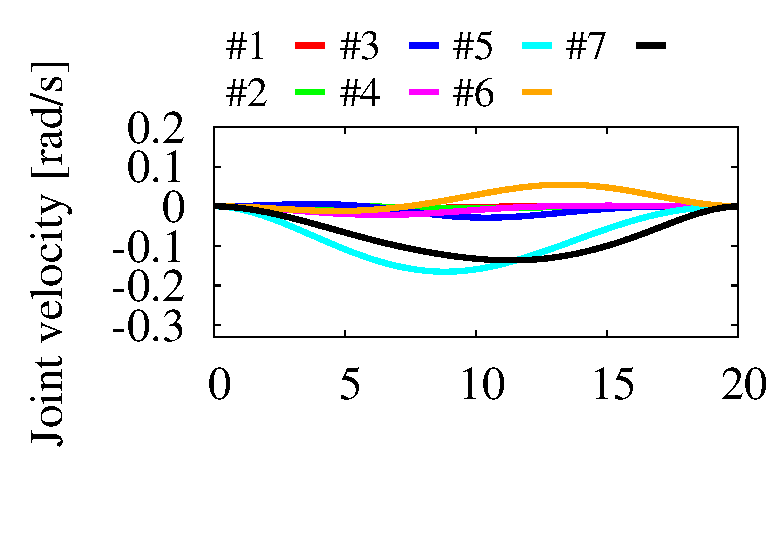
\includegraphics[width=1.0\linewidth]{fig/chapter4/inspection/case1/RL-M/U01_joint_velo.eps}
  \end{minipage}
  \begin{minipage}[h]{0.40\linewidth}
    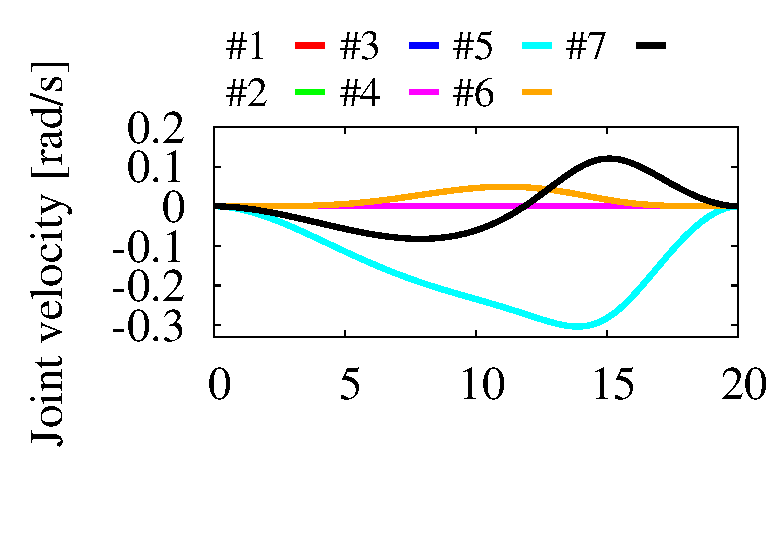
\includegraphics[width=1.0\linewidth]{fig/chapter4/inspection/case1/CONV/U01_joint_velo.eps}
  \end{minipage}\\
  \vspace{-5mm}
  \begin{minipage}[h]{0.40\linewidth}
    \includegraphics[width=1.0\linewidth]{fig/chapter4/inspection/case1/RL-M/U12_rotation_angle.eps}
  \end{minipage}
  \begin{minipage}[h]{0.40\linewidth}
    \includegraphics[width=1.0\linewidth]{fig/chapter4/inspection/case1/CONV/U12_rotation_angle.eps}
  \end{minipage}\\
  \vspace{-5mm}
  \begin{minipage}[h]{0.40\linewidth}
    \centering
    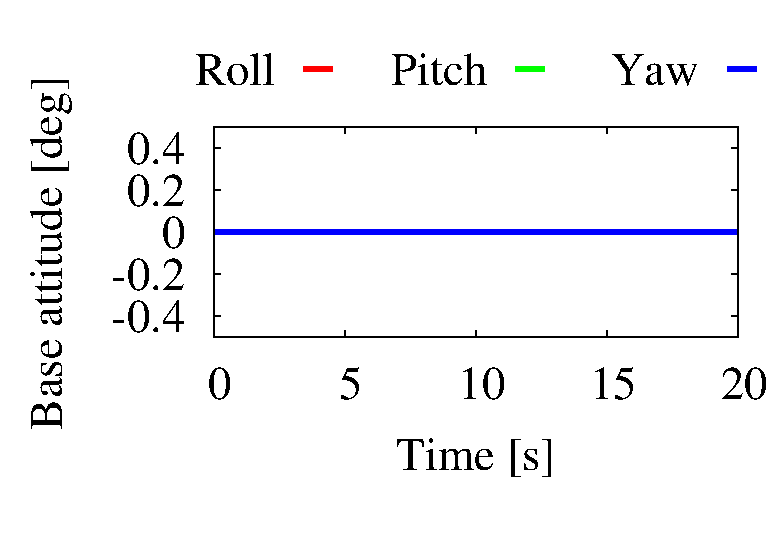
\includegraphics[width=1.0\linewidth]{fig/chapter4/inspection/case1/RL-M/X02_Base_Orientation.eps}
    \footnotesize\par{\hspace{8mm}\vspace{-2mm}Reactionless}
  \end{minipage}
  \begin{minipage}[h]{0.40\linewidth}
    \centering
    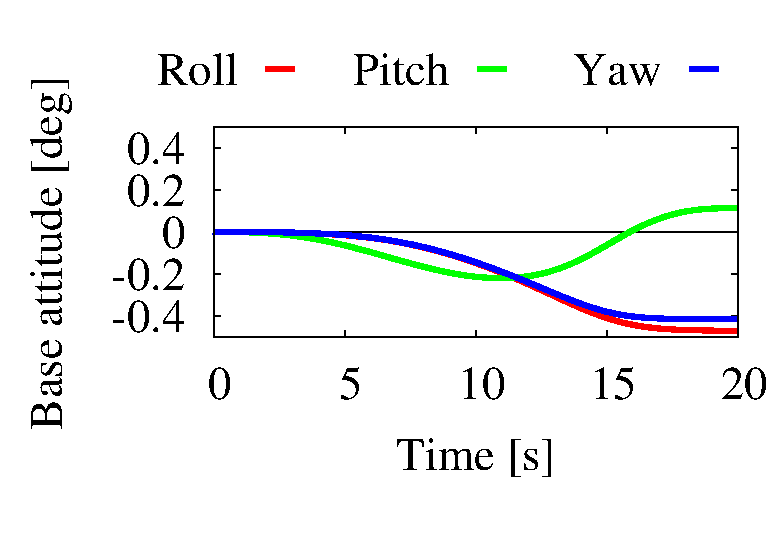
\includegraphics[width=1.0\linewidth]{fig/chapter4/inspection/case1/CONV/X02_Base_Orientation.eps}
    \footnotesize\par{\hspace{8mm}\vspace{-2mm}Conventional}
  \end{minipage}
  \vspace{1em}
  \caption{Simulation result under the satellite observation mission (\fig{ins}~(a)).}
  \label{fig:RES_INS}
\end{figure}
% ---------------------------------------------------------------------
%
We assume the following two task scenarios for observing:
(i)  a satellite to be serviced (\fig{ins}~(a)) and
(ii) the devices attached on  satellite base (\fig{ins}~(b)).
First, we verify the satellite observation case.
The initial configuration is set as $[-90~-30~0~-70~180~-30~0]^{T}\unit{deg}$ as shown in \fig{ins}~(a),
the reference angular velocity is $\bm{\omega}_{e}^{ref} = \pi[s(t)~0~0]^{T}$,
where $0 \leq s(t) \leq 1$ denotes a fifth-order spline function. 
The simulation time and the gain are set at $20\unit{s}$ and $k_{g} = 100  \unit{kg/m \cdot s}$, respectively.
The simulation results are displayed in \fig{RES_INS}.
From the angular velocity error graphs is can be seen that the end-effector task is accomplished successfully
in both simulations. Note, however, that under reactionless motion control there is no base attitude deviation.
Also, this motion is realized with a relatively small displacement of the positioning subchain, 
according to the respective joint velocity graph. In contrast, under the conventional control method
there is a relatively large base attitude deviation% 
\footnote{The maximum allowable base attitude deviation for the ETS-VII mission was about $\pm 0.05\unit{deg}$.}, 
despite the low inertia parameters of the wrist.

%
% ---------------------------------------------------------------------
\begin{figure}[t]
  \centering
  \begin{minipage}[h]{0.40\linewidth}
    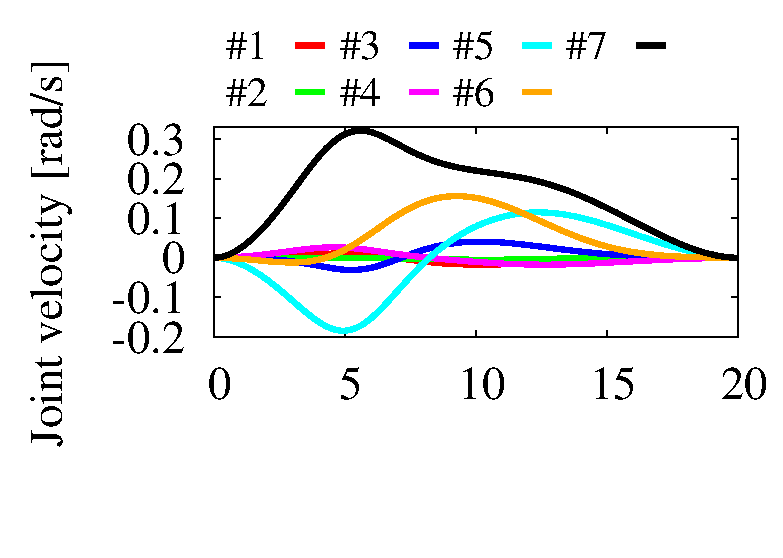
\includegraphics[width=1.0\linewidth]{fig/chapter4/inspection/case2/RL-M/U01_joint_velo.eps}
  \end{minipage}
  \begin{minipage}[h]{0.40\linewidth}
    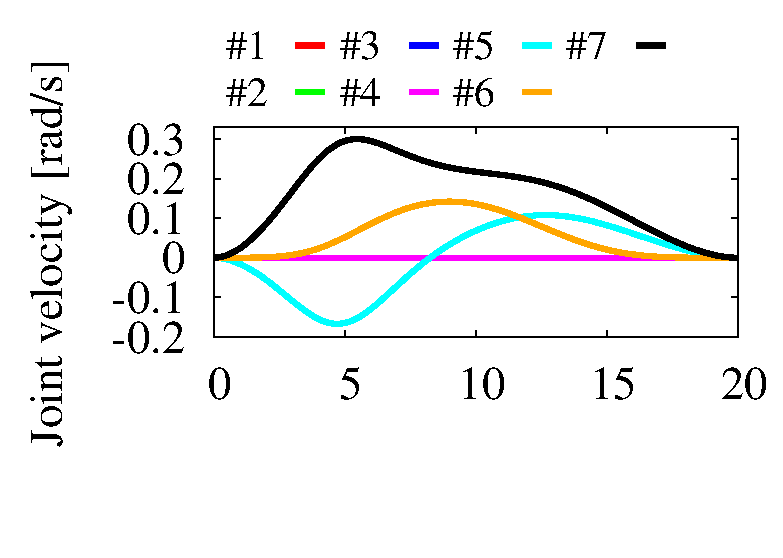
\includegraphics[width=1.0\linewidth]{fig/chapter4/inspection/case2/CONV/U01_joint_velo.eps}
  \end{minipage}\\
  \vspace{-5mm}
  \begin{minipage}[h]{0.40\linewidth}
    \centering
    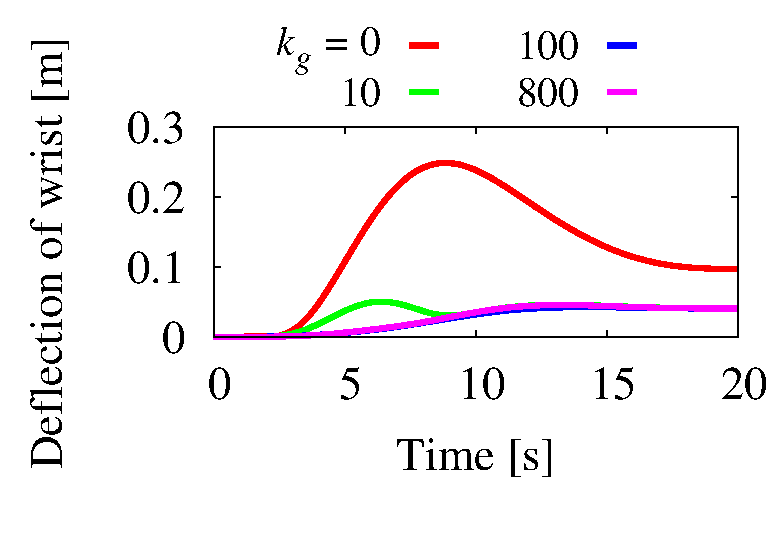
\includegraphics[width=1.0\linewidth]{fig/chapter4/inspection/case2/RL-M/U13_wrist_deflection.eps}
    \footnotesize\par{\hspace{8mm}\vspace{-2mm}Reactionless}
  \end{minipage}
  \begin{minipage}[h]{0.40\linewidth}
    \centering
    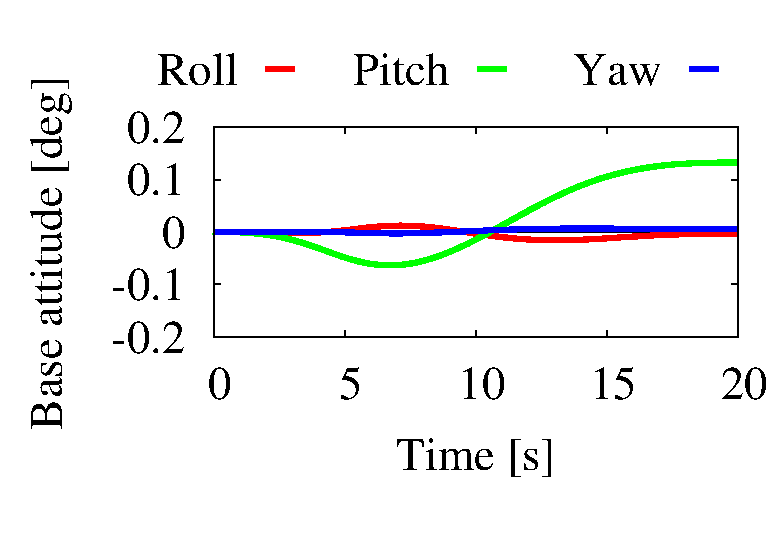
\includegraphics[width=1.0\linewidth]{fig/chapter4/inspection/case2/CONV/X02_Base_Orientation.eps}
    \footnotesize\par{\hspace{8mm}\vspace{-2mm}Conventional}
  \end{minipage}
  \vspace{1em}
  \caption{Simulation result under the inspection of own-satellite mounted devices (\fig{ins}~(b)).}
  \label{fig:RES_INS2}
\end{figure}
% ---------------------------------------------------------------------
%
In the second scenario, 
we assume that the initial configuration is set to $[90~-20~180~110~0~20~0]^{T}\unit{deg}$ as shown in \fig{ins}~(b),
the desired end-effector velocity is $\bm{\omega}_{e}^{ref} = \pi[0~0~-s(t)]^{T}\unit{rad/s}$.
The other conditions are the same as in the previous simulation.
The simulation results are shown in \fig{RES_INS2}.
First, it becomes apparent that also in this case, the base remains undisturbed under reactionless motion
while under conventional control,  a relatively large base attitude deviation is observed. 
Under reactionless motion, the effect of the cost function leads to a sufficiently small deviation from
the initial wrist position as shown in \fig{RES_INS2}.

In summary, a somewhat surprising result was obtained with the conventional controller:
a relatively large base attitude deviation was  observed despite the small mass and inertia moment 
of the wrist subchain. We can then conclude that reactionless camera inspection is useful  
to overcome this problem.

%%%%%%%%%%%%%%%%%%%%%%%%%%%%%%%%%%%%%%%%%%%%%%%%%%%%%%%%%
\section{Singularities within the inspection task}
\label{sec:SINGULAR}
%%%%%%%%%%%%%%%%%%%%%%%%%%%%%%%%%%%%%%%%%%%%%%%%%%%%%%%%%
%%%%%%%%%%%%%%%%%%%%%%%%%%%%%%%%%
\subsection{Problem statement}
\label{sec:PROBLEM}
%%%%%%%%%%%%%%%%%%%%%%%%%%%%%%%%%
In this section, we deal with possible singularities that could be encountered during 
the proposed reactionless task. There are three types of such singularities, as follows:
\begin{itemize}
\item Kinematic singularity: $\mathrm{det}(\bm{J}_{\omega_{e}}\bm{J}_{\omega_{e}}^{T}) = 0$.
\item Singularities of the coupling inertia matrix: $\mathrm{det}(\tbm{M}_{\omega m}\tbm{M}_{\omega m}^{T}) = 0$.
\item Algorithmic singularities: $\mathrm{det}(\bar{\bm{J}}_{\omega_{e}}\bar{\bm{J}}_{\omega_{e}}^{T}) = 0$
with non-singular $\bm{J}_{\omega_{e}}$ and full row-rank $\tbm{M}_{\omega m}$.
\end{itemize}
%
Kinematic singularities have been much discussed by various researchers, 
e.g.\ \cite{Kreutz-Delgado1992, Boudreau2010}. The damped least-squares  (DLS) method
was applied \cite{Nakamura1986,Wampler1986} to deal with these type of singularity.  
The infinite growth  of the joint velocity in the neighborhood of a singularity can be suppressed 
by a suitably defined  damping factor. This method, however, has some drawbacks \cite{Nenchev1996}: it causes 
workspace errors both in speed and motion direction. In addition, the determination of the damping factor is 
counter-intuitive. Another method,  called the Singularity Consistent method, was proposed in \cite{Nenchev2000}.
Under this method, the manipulator can follow the desired path exactly, without causing a large joint velocity%
\footnote{The term ``path'' should be distinguished from ``trajectory'':
the former is characterized only geometrically while the latter includes  time/velocity 
relations.}.

In contrast, the second and third types of singularities  have not been discussed extensively, so far.
Fortunately, the singularities of the coupling inertia matrix do not pose a problem here
because we use the null-space of the coupling inertia matrix.
Indeed, in \eq{REF} the rank of restricted Jacobian $\bar{\bm{J}}_{\omega_{e}}$ depends upon the conditioning 
of $\bm{J}_{\omega_{e}}$ only, since ${\rm rank}\bm{P}_{RNS}$ grows when ${\rm rank} \bm{J}_{\omega_{e}}$
decreases. %Hence, there is no need to pay attention to this type of singularity.

On the other hand,  algorithmic singularities should be handled with care.
There are few studies that treat this type of singularities.
In \cite{Agrawal1995}, the algorithmic singularities of a planar six-DoF dual arm model were discussed.
For reactionless motion control of flexible base robots,
a singularity treatment technique was proposed in \cite{Hara2010}.
However, these two methods cannot be applied in our case.

Using SVD, the (pseudo)inverse of $\bar{\bm{J}}_{\omega_{e}}$ can be written as:
%
% ---------------------------------------------------------------------
\begin{align}
  \bar{\bm{J}}_{\omega_{e}}^{+} = \frac{1}{\sigma_{1}}\bm{v}_{1}\bm{u}_{1}^{T} + 
  \frac{1}{\sigma_{2}}\bm{v}_{2}\bm{u}_{2}^{T} + 
  \frac{1}{\sigma_{3}}\bm{v}_{3}\bm{u}_{3}^{T}\label{eq:JP_SVD}
\end{align}
% ---------------------------------------------------------------------
%
where  $\sigma_{1} \geq \sigma_{2} \geq \sigma_{3}$ are the singular values,
$\bm{v}_{i}\R{7}$, $\bm{u}_{i}\R{3}$ are the left and right singular vectors
associated with $\sigma_{i}$. In the neighborhood of a singularity where $\sigma_{3}$ approaches zero,
the last term attains an extremely large value.

In what follows, an example of an algorithmic singularity will be presented.
The initial configuration is the same as  in the satellite observation task (cf.\ \fig{ins}~(a)).
The commanded angular velocity is however different:  $\bm{\omega}_{e}^{ref} = [0~-0.2~0]^{T}\unit{rad/s}$.
The simulation results are displayed in \fig{RES_SIN}.

% ---------------------------------------------------------------------
\begin{figure}[t]
  \centering
  \begin{minipage}[t]{0.40\linewidth}
    \centering
    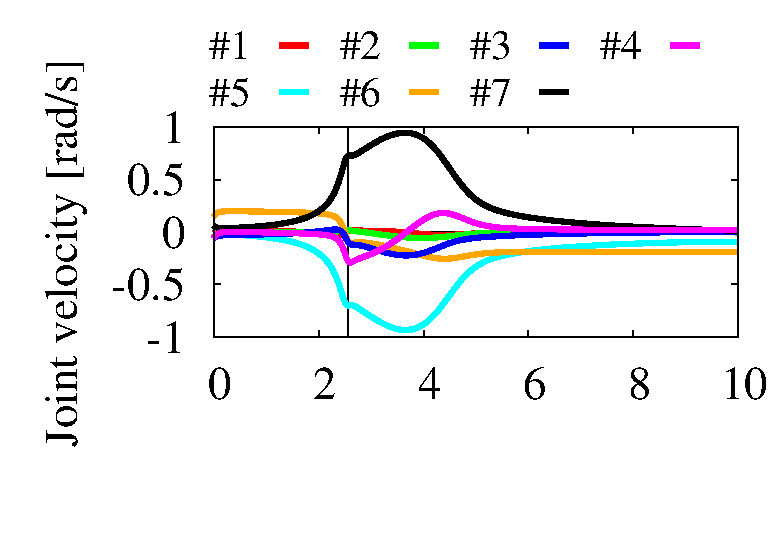
\includegraphics[width=1.0\linewidth]{fig/chapter4/inspection/singularity/SAMPLE/U01_joint_velo.eps}
  \end{minipage}
  \begin{minipage}[t]{0.40\linewidth}
    \centering
    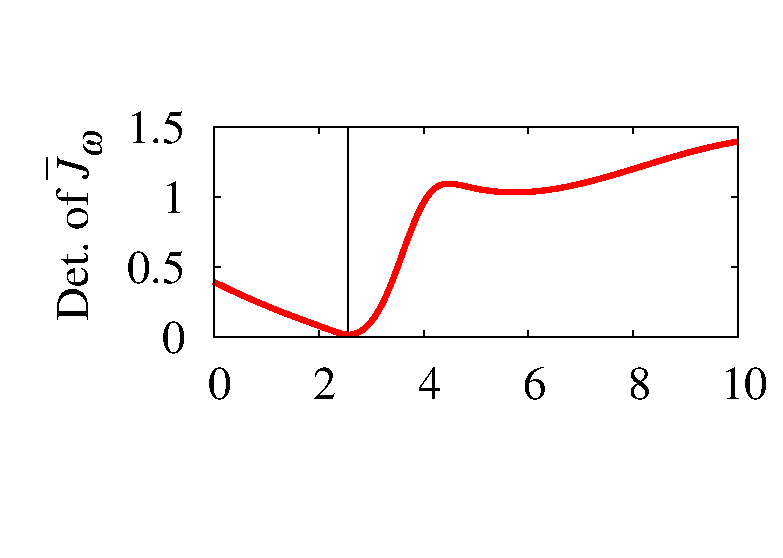
\includegraphics[width=1.0\linewidth]{fig/chapter4/inspection/singularity/SAMPLE/U16_determinant_Gw.eps}
  \end{minipage}\\
  \vspace{-5mm}
  \begin{minipage}[t]{0.40\linewidth}
    \centering
    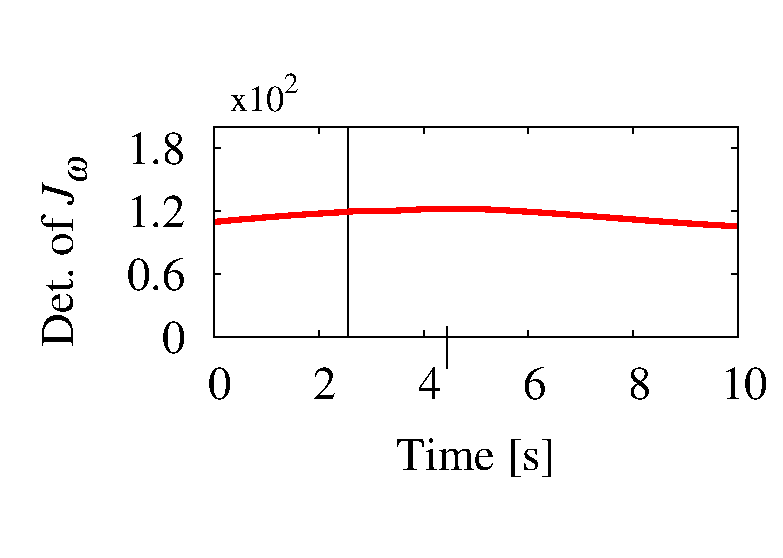
\includegraphics[width=1.0\linewidth]{fig/chapter4/inspection/singularity/SAMPLE/U14_determinant_Jw.eps}
  \end{minipage}
  \begin{minipage}[t]{0.40\linewidth}
    \centering
    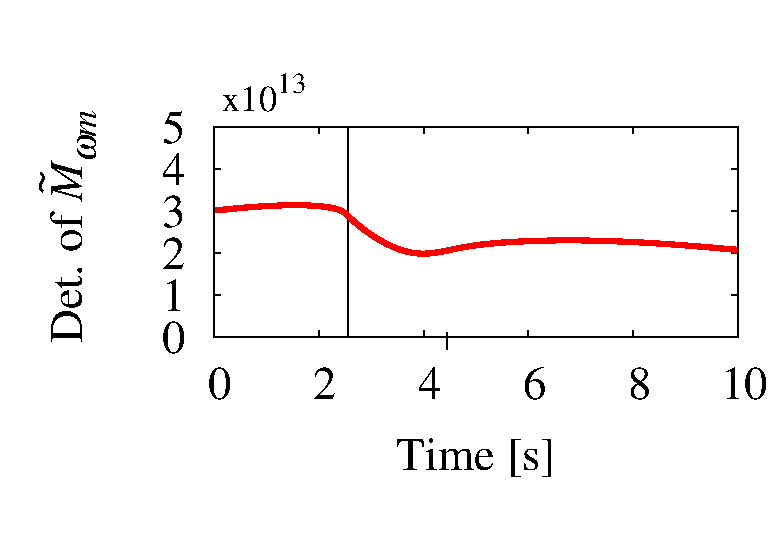
\includegraphics[width=1.0\linewidth]{fig/chapter4/inspection/singularity/SAMPLE/U15_determinant_Mwm.eps}
  \end{minipage}
  \caption{An example of the algorithmic singularity within the proposed method.}
  \label{fig:RES_SIN}
\end{figure}
% ---------------------------------------------------------------------
%
In the graphs, the vertical line represents the time instant when
the manipulator is passing  near a singularity whereby
$\det(\bar{\bm{J}}_{\omega_{e}}\bar{\bm{J}}_{\omega_{e}}^{T})$ approaches zero but the other two 
determinants,  $\mathrm{det}(\bm{J}_{\omega_{e}}\bm{J}_{\omega_{e}}^{T})$ and
$\mathrm{det}(\tbm{M}_{\omega m}\tbm{M}_{\omega m}^{T})$, do not. %  as shown in \fig{RES_SIN}.
Hence, this singularity can be recognized as an algorithmic one.
From the joint velocity graphs it is seen that near the singularity, 
Joints 5 and 7 rotate in opposite directions with high  joint rates.
This type of behavior is observed at singularities of the Euler angles \cite{Taki2013}
as well as at wrist singularities \cite{Aboaf1987}.

From our observation, it seems that such algorithmic  singularities do not occur frequently.
But nevertheless, we will show that singularity treatment techniques such as  the DLS and 
Singularity Consistent methods, can be effective w.r.t.\ algorithmic singularities.

%%%%%%%%%%%%%%%%%%%%%%%%%%%%%%%%%%%%%%%%%%%%%%%%%%%%%%%%%%%%%%%%%%%%%%%%%
\subsection{Singularity treatment with the Damped Least-Squares inverse}
\label{sec:SIN_DLS}
%%%%%%%%%%%%%%%%%%%%%%%%%%%%%%%%%%%%%%%%%%%%%%%%%%%%%%%%%%%%%%%%%%%%%%%%%
Originally, the DLS generalized inverse is obtained by  adding damping factors to the  denominators
in \eq{JP_SVD} to suppress high  joint rates.  We resume, however, to a DLS inverse that 
is obtained with a so-called  numerical filtering technique \cite{Chiaverini1997}. This approach can alleviate  
the problem of large errors. Accordingly, 
the generalized inverse of $\bar{\bm{J}}_{\omega_{e}}$ is obtained in the following form:
%
% ---------------------------------------------------------------------
\begin{align}
  \bar{\bm{J}}_{\omega_{e}}^{\#} = \bar{\bm{J}}_{\omega_{e}}^{T}\Big(\bar{\bm{J}}_{\omega_{e}}\bar{\bm{J}}_{\omega_{e}}^{T} +
  \lambda^{2}\bm{u}_{3}\bm{u}_{3}^{T}\Big)^{-1}\label{eq:INV_DAMPED}
\end{align}
% ---------------------------------------------------------------------
%
where  $\lambda$ is a damping factor,
$\bm{u}_{3}\R{3}$ is the left singular vector associated with the minimum singular value $\sigma_{3}$,
$(\circ)^{\#}$ represents the DLS inverse. 
%By replacing the pseudoinverse solution with the DLS one,we can deal with the singularity problem.
Further on, through SVD \eq{INV_DAMPED} can be rewritten as:
%
% ---------------------------------------------------------------------
\begin{align}
  \bar{\bm{J}}_{\omega_{e}}^{\#} = \sum_{i = 1}^{2}\frac{1}{\sigma_{i}}\bm{v}_{i}\bm{u}_{i}^{T} +
  \frac{\sigma_{3}}{\sigma_{3}^{2} + \lambda^{2}}\bm{v}_{3}\bm{u}_{3}^{T}\label{eq:INV_SVD}
\end{align}
% ---------------------------------------------------------------------
%
where $\sigma_{1} \geq \sigma_{2} \geq \sigma_{3}$ are the singular values of $\bar{\bm{J}}_{\omega_{e}}$ and
$\bm{u}_{i}\R{3}$, $\bm{v}_{i}\R{7}$ are the associated left and right singular vectors.
Compared with \eq{JP_SVD}, it can be seen that the DLS inverse with numerical filtering
is characterized by inserting  a damping factor  only into the last term, with the 
minimum singular value. Hence, compared to the original DLS inverse
which adds damping into all terms, the error of the solution can be reduced \cite{Chiaverini1997}.
%
% ---------------------------------------------------------------------
\begin{figure}[t]
  \centering
  \begin{minipage}[h]{0.40\linewidth}
    \centering
    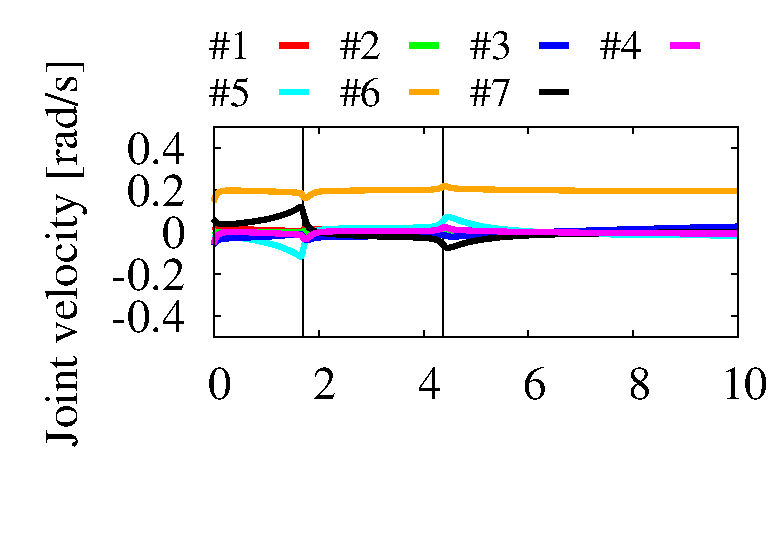
\includegraphics[width=1.0\linewidth]{fig/chapter4/inspection/singularity/DLS/U01_joint_velo.eps}
  \end{minipage}
  \begin{minipage}[h]{0.40\linewidth}
    \centering
    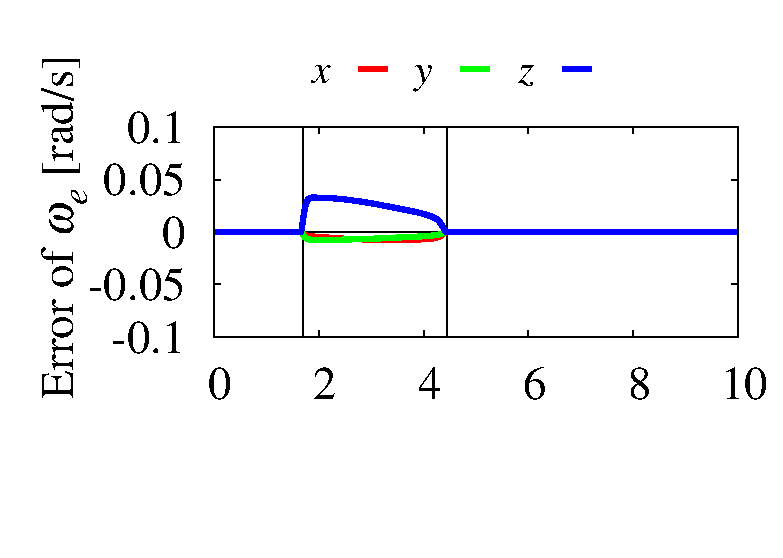
\includegraphics[width=1.0\linewidth]{fig/chapter4/inspection/singularity/DLS/U20_EE_vel_error.eps}
  \end{minipage}\\
  \vspace{-7mm}
  \begin{minipage}[h]{0.40\linewidth}
    \centering
    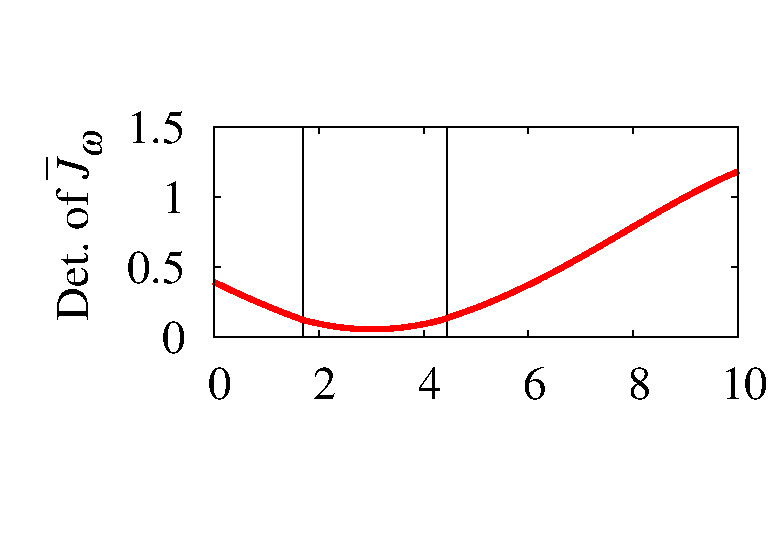
\includegraphics[width=1.0\linewidth]{fig/chapter4/inspection/singularity/DLS/U16_determinant_Gw.eps}
  \end{minipage}
  \begin{minipage}[h]{0.40\linewidth}
    \centering
    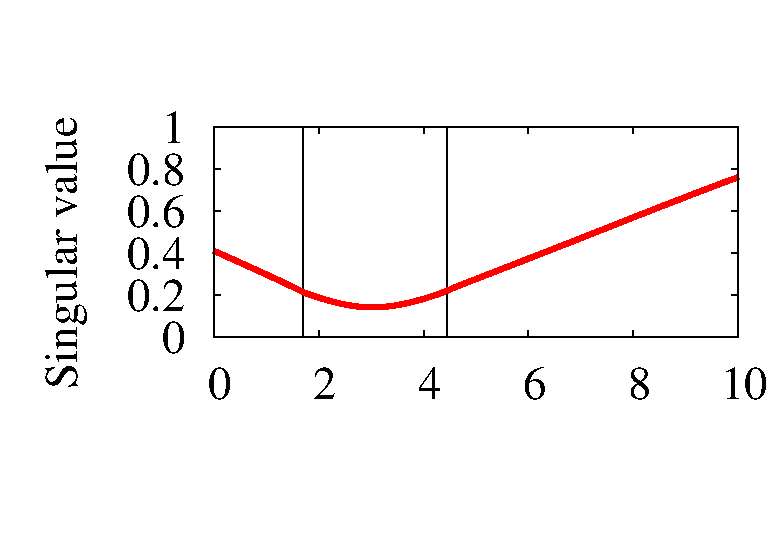
\includegraphics[width=1.0\linewidth]{fig/chapter4/inspection/singularity/DLS/U18_minimal_singular_value.eps}
  \end{minipage}\\
  \vspace{-7mm}
  \begin{minipage}[h]{0.40\linewidth}
    \centering
    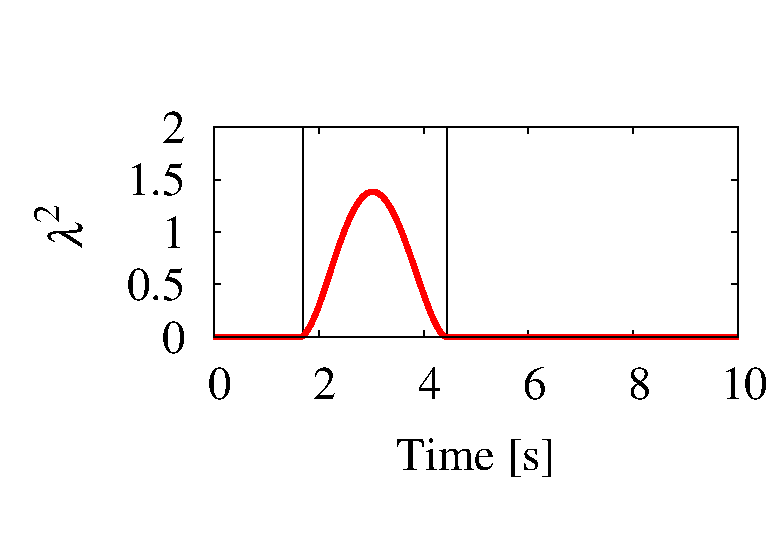
\includegraphics[width=1.0\linewidth]{fig/chapter4/inspection/singularity/DLS/U19_interpolation.eps}
  \end{minipage}
  \begin{minipage}[h]{0.40\linewidth}
    \centering
    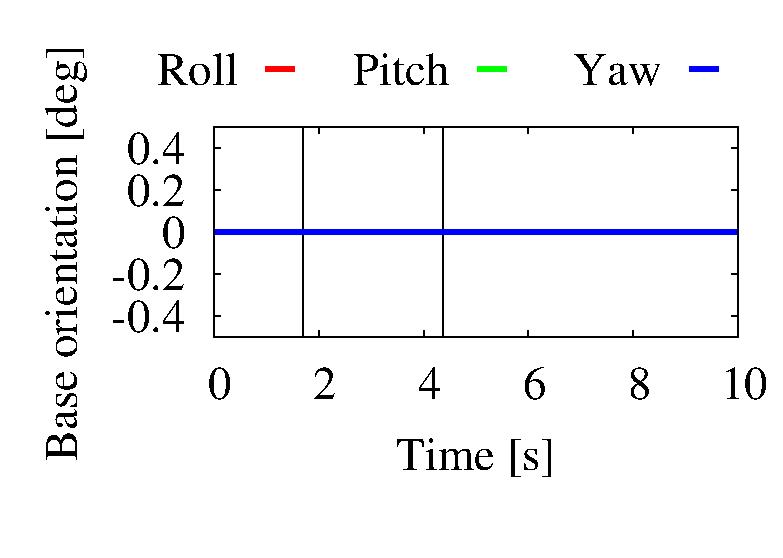
\includegraphics[width=1.0\linewidth]{fig/chapter4/inspection/singularity/DLS/X02_Base_Orientation.eps}
  \end{minipage}
  \caption{Simulation results under the damped least-squares inverse with numerical filtering.}
  \label{fig:RES_DLS}
\end{figure}
% ---------------------------------------------------------------------
%
Based on \cite{Chiaverini1994},
the damping factor is obtained as follows:
%
% ---------------------------------------------------------------------
\begin{align}
   \lambda^{2} &= \begin{cases} 0 & \varepsilon < \sigma_{3} \\
    (1 - \frac{2\sigma^{2}_{3}}{\varepsilon^{2}} + \frac{\sigma_{3}^{4}}{\varepsilon^{4}})\lambda_{max}^{2}
   & \sigma_{3} \leq \varepsilon\label{eq:damper}
  \end{cases}
\end{align}
% ---------------------------------------------------------------------
%
where  $\varepsilon$ defines the singular region,
which is introduced in the neighborhood of the singularity,
$\lambda_{max}$ sets the maximum value of the damping factor.
Note that we added an additional term, the $\sigma_{3}^{4}$ related term, 
into \eq{damper} to obtain a smooth transition at the border of the singular region.
%The original one did not consider the continuity at the first differential in 
%terms of $\sigma_{3}$.

The performance of the DLS inverse for this controller
is verified via numerical simulation.
The simulation conditions are the same as in \sec{PROBLEM}.
The singular region is defined by $\varepsilon = 0.2$ and
the maximum damping value set at $\lambda_{max}^{2} = 2$.
The results are displayed in \fig{RES_DLS}.
In the graphs, the singular region is indicated by the two vertical lines 
($1.71\unit{s} \leq t \leq 4.18\unit{s}$). From the results it is apparent that
the growth of the joint velocity has been successfully suppressed through the damping factor.
However, an end-effector tracking error can be observed within the singular region.
This is caused by the damping factor, as already explained. On the other hand,
the base attitude does not deviate, even within the singular region.


%%%%%%%%%%%%%%%%%%%%%%%%%%%%%%%%%%%%% HERE %%%%%%%%%%%%%%%%%%%%%%%%%%%%%%%%%%%%
\subsubsection{The Singularity Consistent method}
\label{sec:SIN_SC}
%%%%%%%%%%%%%%%%%%%%%%%%%%%%%%%%%%%%%%%%%%%%%%%%%%%%%%%%%%%%%%%%%%%%%%%%%
We will examine the possibility to make use of the Singularity Consistent (SC) method
for singularity treatment. It was clarified that the DLS method introduces an error
in the direction of motion since the singular direction, i.e.\ $\bm{v}_{3}$, has to 
be avoided. In contrast,
the SC method actively makes use of this direction and therefore, 
the manipulator can follow the direction of the desired end-effector velocity, correctly.
An error only appears in the speed along the path. If we consider a teleoperation task,
such an error is not a problem because the operator can modify the desired end-effector speed
according to the task conditions. Teleoperation under the SC method is discussed  in 
\cite{Tsumaki1997,Tsumaki1998}.

We will make use of natural motion \cite{Nenchev2007,Nenchev2010}, i.e.\ 
end-effector motion with velocity in proportion to
the determinant of the Jacobian matrix. There is no need to define a singular region then, and hence,
to switch the control input.

According to the SC method,  the inverse of $\bar{\bm{J}}_{\omega_{e}}$ can be obtained as follows:
%
% ---------------------------------------------------------------------
\begin{align}
  \bar{\bm{J}}_{\omega_{e}}^{+} &= b\sum_{i=1}^{3}\mu_{i}\bm{v}_{i}\bm{u}_{i}^{T}\label{eq:SC_INV}\\
  \mu_{i} &= \prod_{j=1, j\not = i}^{3}\sigma_{i}\label{eq:SC_SV}
\end{align}
% ---------------------------------------------------------------------
%
where $b$ is a constant scalar. From \eq{SC_SV},
we can see that $\mu_{1}$ and $\mu_{2}$ become small near the singularity,
because their values are proportional to the minimum singular value that approaches $0$ in the 
vicinity of the singularity. Hence, the $\bm{v}_{3}$ related term is actively used.

We verify the performance of this method through numerical simulation.
The simulation conditions are the same as in the DLS case. 
Empirically, the constant scalar was set to $b = 1.7$.
In addition, to avoid a large joint velocity obtained from the null-space term,
we multiply the term by the determinant of $\bar{\bm{J}}_{\omega_{e}}\bar{\bm{J}}_{\omega_{e}}^{T}$ as follows:
%
% ---------------------------------------------------------------------
\begin{align}
  \thd^{ref} = \bar{\bm{J}}_{\omega_{e}}^{+}\bm{\omega}_{e}^{ref} + 
k_{g}\mathrm{det}(\bar{\bm{J}}_{\omega_{e}}\bar{\bm{J}}_{\omega_{e}}^{T})\bm{P}(\bm{J}_{v_{w}}^{T})\Delta\bm{p}_{w}
\end{align}
% ---------------------------------------------------------------------
%
The simulation results are displayed in \fig{RES_SC}.
The results show that the rapid change of the joint velocity can be avoided.
In addition to this feature, it is seen that the end-effector  follows the desired 
velocity direction $y$, which is in contrast with the result from the DLS simulation.
Hence, adjustment of the speed is only needed by the operator under teleoperation.

%
% ---------------------------------------------------------------------
\begin{figure}[t]
  \centering
  \begin{minipage}[h]{0.40\linewidth}
    \centering
    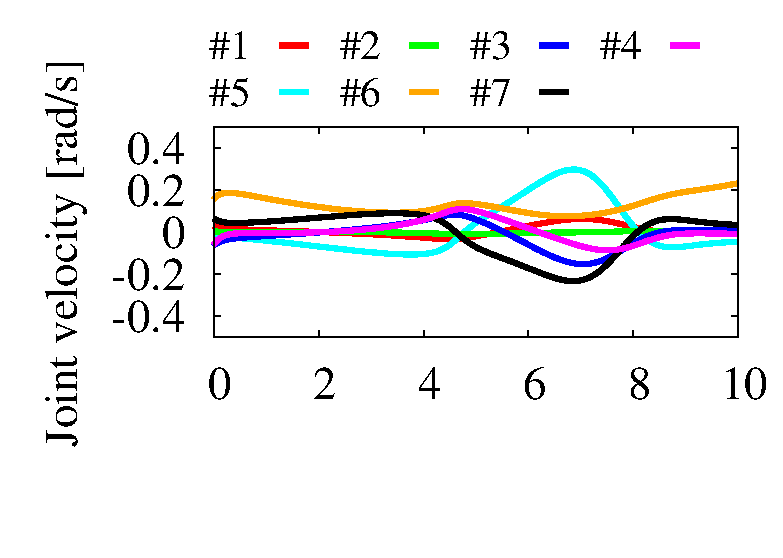
\includegraphics[width=1.0\linewidth]{fig/chapter4/inspection/singularity/SC/U01_joint_velo.eps}
  \end{minipage}
  \begin{minipage}[h]{0.40\linewidth}
    \centering
    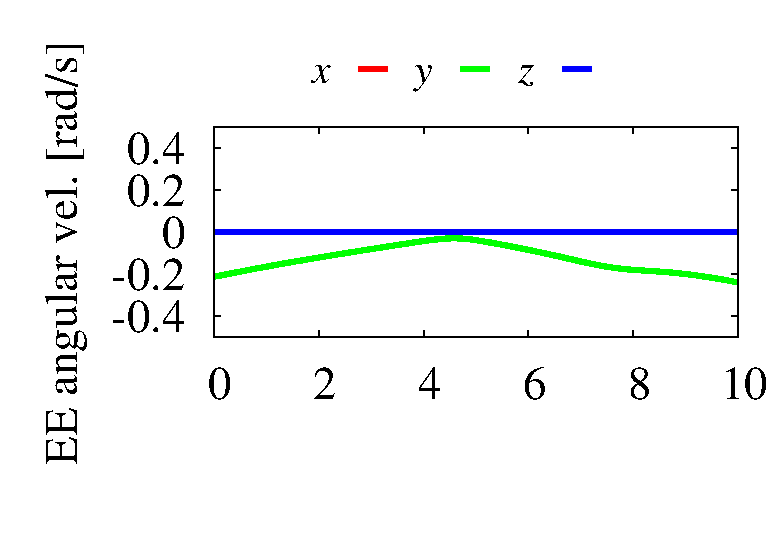
\includegraphics[width=1.0\linewidth]{fig/chapter4/inspection/singularity/SC/U08_end_tip_ang_vel.eps}
  \end{minipage}\\
  \vspace{-5mm}
  \begin{minipage}[h]{0.40\linewidth}
    \centering
    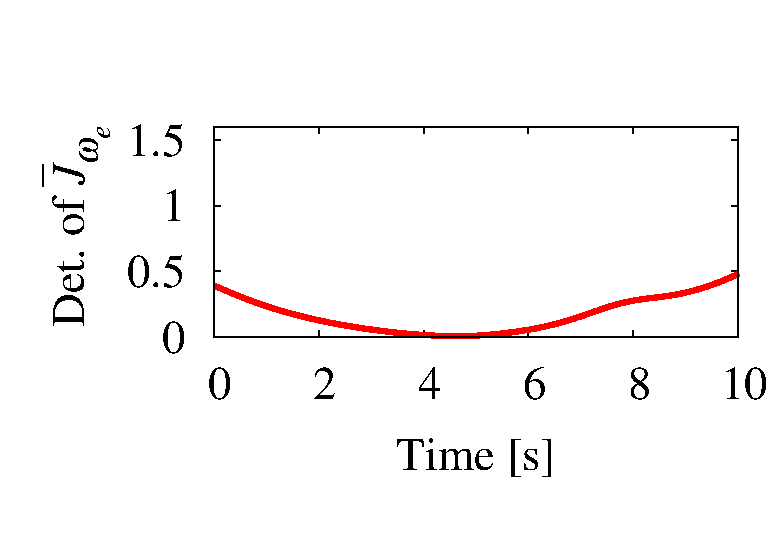
\includegraphics[width=1.0\linewidth]{fig/chapter4/inspection/singularity/SC/U16_determinant_Gw.eps}
  \end{minipage}
  \begin{minipage}[h]{0.40\linewidth}
    \centering
    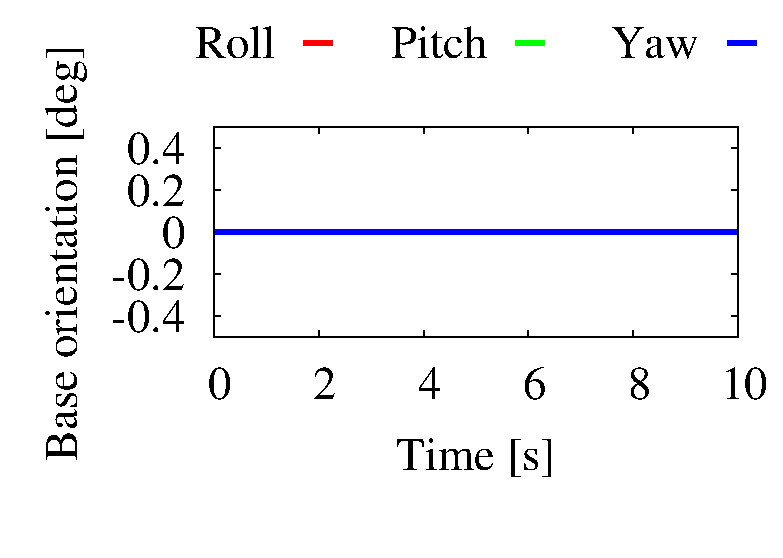
\includegraphics[width=1.0\linewidth]{fig/chapter4/inspection/singularity/SC/X02_Base_Orientation.eps}
  \end{minipage}
  \caption{Simulation results under the singularity consistent method.}
  \label{fig:RES_SC}
\end{figure}
% ---------------------------------------------------------------------
%



%%%%%%%%%%%%%%%%%%%%%%%%%%%%%%%%%%%%%%%%%%%%%%%%%%%%%
\section{Point-to-point positioning task}
%%%%%%%%%%%%%%%%%%%%%%%%%%%%%%%%%%%%%%%%%%%%%%%%%%%%%
As the second reactionless task,
we focus on point-to-point (PTP) positioning tasks of the end-effector.
PTP positioning tasks would be used several situation such as
pre-positioning task of the camera inspection, assembly and so on.
Among the several positioning tasks,
we restrict our attention to a specific subset of PTP tasks:
arm reconfiguration tasks wherein the hand does not hold an object.
It would be desirable to execute such tasks under reactionless motion control.

However,
this is impossible for arbitrary points since reactionless motions are quite restricted.
Nevertheless, reactionless motion can be useful if the PTP motion is planned appropriately.
One possibility is to combine two reactionless motions with a non-restricted PTP motion 
that induces the base disturbance.
This method was originally proposed in \cite{Yoshida1996};
it has been referred to as the \textit{3-Phase method} and
applied to a planar flexible base robots.
Note that despite the advantage of the method was
verified with a planar flexible base robots,
the cases of free-floating base robots and also
three-dimensional models have not been discussed before.
We verify the performance of this method with the three-dimensional free-floating robot.

%%%%%%%%%%%%%%%%%%%%%%%%%%%%%%%%%%%%%
\subsection{The 3-Phase method}
%%%%%%%%%%%%%%%%%%%%%%%%%%%%%%%%%%%%%

%
% ---------------------------------------------------------------------
\begin{figure}[t]
  \centering
  \begin{minipage}[h]{0.8\linewidth}
    \centering
    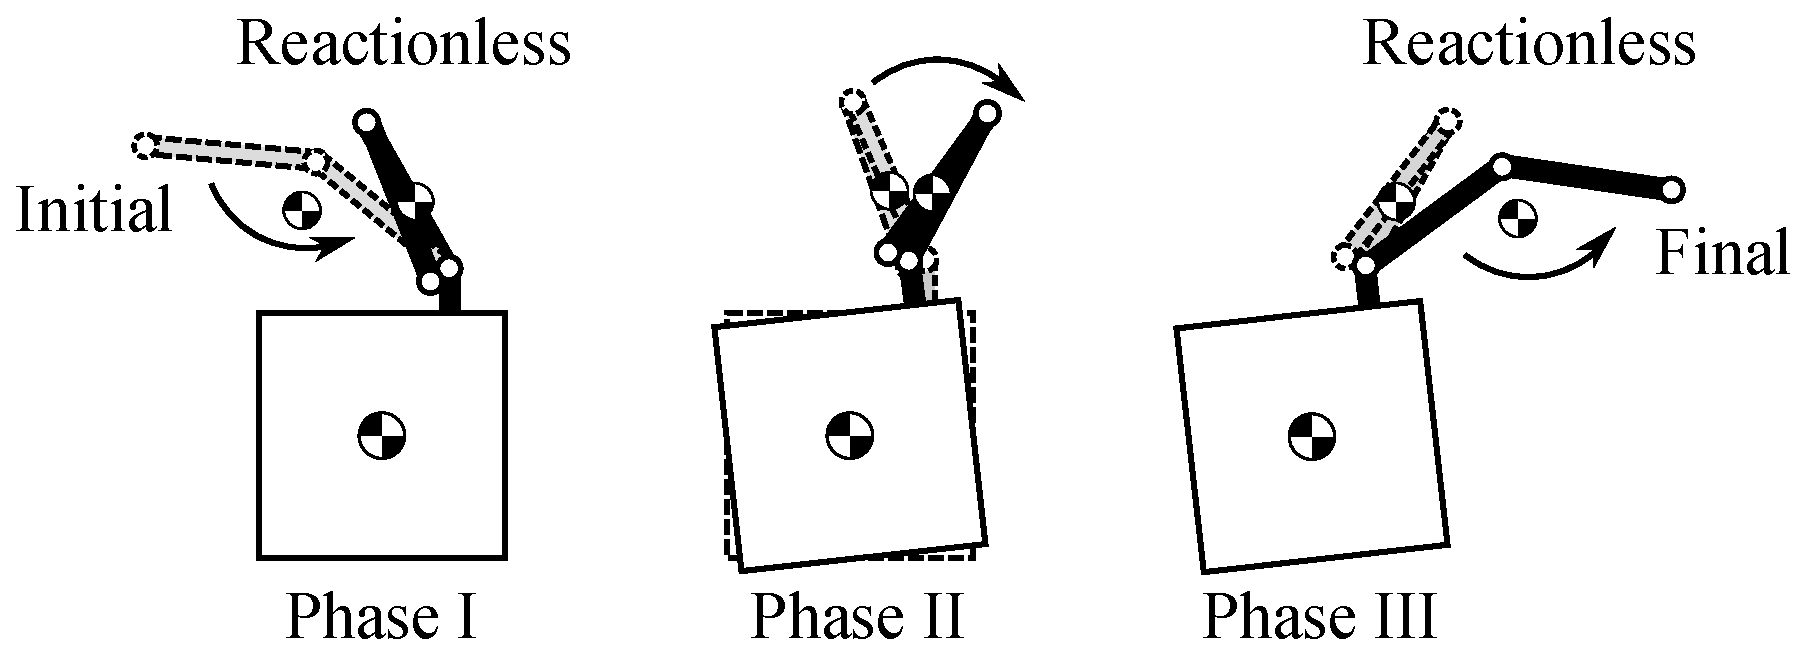
\includegraphics[width=1.0\linewidth]{fig/chapter4/PTP/motion.eps}
  \end{minipage}
  \caption{A motion obtained via the 3-Phase method.}
  \label{fig:3PHASE}
\end{figure}
% ---------------------------------------------------------------------
%
First, we review the 3-Phase method.
The 3-Phase method deals with the following issue:
find a joint path that connects specific initial and final configurations
with three sub-paths.
We divide a motion into three Phase, which are Phase I, II and III, according to the three sub-paths.
In Phase I and III,
reactionless motion is used.
In Phase II,
these two reactionless motion paths are connected via a joint path that is not reactionless.
% A graphical image of the 3-Phase method is depicted in \fig{3PHASE}.
The primary concern is how to determine the three sub-paths to obtain small base disturbance
during the PTP sub-paths in Phase II.
In \cite{Yoshida1996},
a folded arm configuration as shown in \fig{3PHASE} was employed in Phase II.
Using this configuration, the base disturbance can be reduced.
We provide a theoretical argument of reaction reduction with the folded configuration in what follows.
The coupling angular momentum, which is the base reaction with dimension of momentum,
can be represented in the following form:
%
% ---------------------------------------------------------------------
\begin{align}
  \tilde{\bm{M}}_{\omega m}\dot{\bm{\theta}} &= \Big\{\sum_{i = 1}^{n}\bm{I}_{i}\bm{J}_{\omega_{i}}\Big\}\dot{\bm{\theta}}~ + \notag\\
  &\Big\{\sum_{i=1}^{n}m_{i}[\bm{r}_{b \rightarrow i}^{\times}]\bm{J}_{v_{i}}\Big\}\thd -
  \Big\{m_{c}[\bm{r}_{b \rightarrow c}^{\times}]\bm{J}_{c}\Big\}\thd,
  \label{eq:CIM}
\end{align}
% ---------------------------------------------------------------------
%
It is apparent that the coupling angular momentum consists of three kinds of angular momentum.
The first term represents the angular momentum induced by
purely rotational motion of each link;
the second and third term are the angular momentum arising from the moment of the linear momentum
of each link and the CoM of the manipulator.
The coefficient matrix of the first term is related to the inertia tensor of the manipulator.
Hence, at the folded configuration,
this term becomes the smallest value.
On the other hand,
the second and third term are related to the CoM positions.
The base reaction related to these term also takes small amount
using the folded configuration,
because the distance along which the manipulator CoM moves becomes short,
as shown in \fig{3PHASE}.
In addition,
the norm of $\bm{r}_{b \rightarrow i}$ and $\bm{r}_{b \rightarrow c}$ become small value at the configuration.
Hence, the angular momentum related to the linear momentum of each link can be reduced.
For this reason, the folded configuration is used in Phase II.

% %
% % ---------------------------------------------------------------------
% \begin{figure}[t]
%   \centering
%   \begin{minipage}[h]{0.3\linewidth}
%     \centering
%     \includegraphics[width=1.0\linewidth]{fig/chapter4/PTP/Phase1.eps}
%     \footnotesize\par{\hspace{16mm}Phase I}
%   \end{minipage}
%   \hspace{4mm}
%   \begin{minipage}[h]{0.3\linewidth}
%     \centering
%     \includegraphics[width=1.0\linewidth]{fig/chapter4/PTP/Phase2.eps}
%     \footnotesize\par{Phase II}
%   \end{minipage}
%   \begin{minipage}[h]{0.245\linewidth}
%     \centering
%     \includegraphics[width=1.0\linewidth]{fig/chapter4/PTP/Phase3.eps}
%     \footnotesize\par{\vspace{-0.7mm}Phase III}
%   \end{minipage}
%   \caption{A motion obtained via the 3-Phase method.}
%   \label{fig:3PHASE}
% \end{figure}
% % ---------------------------------------------------------------------
% %



%%%%%%%%%%%%%%%%%%%%%%%%%%%%%%%%%%%%%%%%%%%%%%%%%%%%%
\subsection{Verification via numerical simulations}
%%%%%%%%%%%%%%%%%%%%%%%%%%%%%%%%%%%%%%%%%%%%%%%%%%%%%
%
% ---------------------------------------------------------------------
\begin{figure}[t]
  \centering
  \begin{minipage}[h]{0.4\linewidth}
    \centering
    \includegraphics[width=1.0\linewidth]{fig/chapter4/PTP/3phase/U01_joint_velo_1-4.eps}
    \footnotesize\par{(a)}
  \end{minipage}
  \begin{minipage}[h]{0.4\linewidth}
    \centering
    \includegraphics[width=1.0\linewidth]{fig/chapter4/PTP/3phase/U04_coup_ang_mom.eps}
    \footnotesize\par{(b)}
  \end{minipage}
  \caption{The simulation results under the 3-phase method:
  (a) the joint velocity and (b) the coupling angular momentum.}
  \label{fig:RES_3PHASE}
\end{figure}
% ---------------------------------------------------------------------
%
We verify the performance of the 3-Phase method via numerical simulations,
compared with several conventional controllers.
The initial configuration is $[-20~-40~0~-60~180~180~0]^{T}\unit{deg}$;
the final one is $[-120~50~0~-60~180~180~0]^{T}\unit{deg}$.
Note that these two configurations cannot be linked via reactionless motion.
The motion in Phase I is obtained from the initial configuration toward
a folded configuration (FA-1).
Phase III is determined as a reversed (reactionless) motion starting from the final configuration toward
other folded configuration (FA-2).
These two reactionless motions are obtained as the second term in \eq{RL_POS} as follows:
%
% ---------------------------------------------------------------------
\begin{align}
  \thd^{ref} &= \frac{\dot{\theta}_{4}^{ref}(t)}{n_{4}}\bmat{\bm{n} \\ \bm{0}}\\
  \dot{\theta}_{4}^{ref}(t) &= \dot{\theta}_{4}^{des}(t) + k\Delta\theta_{4}(t)
  \label{eq:PS_MOTION}
\end{align}
% ---------------------------------------------------------------------
%
where $n_{4}$ is the forth element of $\bm{n}$,
$\theta_{4}(t)^{des}$ is the desired trajectory of joint 4;
$\Delta\theta_{4}(t) = \theta_{4}^{des}(t) - \theta_{4}$ is the tracking error.
$k$ is a feedback gain.
The two folded configurations are distinct and uniquely defined as resultant configurations
along the respective reactionless motion, wherein $\theta_{4} = -\pi\unit{rad}$.
In Phase I and III,
the motions were executed in $5\unit{s}$,
and Phase II in $20\unit{s}$.

For the comparison,
the same positioning task was executed under the joint space interpolation with straight line (JS-C),
the inverse Jacobian controller (IJ-C) and the transposed Jacobian controller (TJ-C).
For the task space controllers (IJ and TJ-C),
the final condition was set to the final position of the end-effector in the 3-Phase method as
$[-1.7~0.45~1.7]^{T}\unit{m}$.
The three controllers were executed in $30\unit{s}$.
Note that orientation of the end-effector is not considered for the sake of simplicity.
Hence, only the positioning subchain was driven.

First, we show the results obtained in the 3-Phase method in \fig{RES_3PHASE}.
From the results,
the joint motion can be smoothly obtained and only Phase II introduced the coupling angular momentum.
%
% ---------------------------------------------------------------------
\begin{figure}[t]
  \centering
  \begin{minipage}[h]{0.3\linewidth}
    \centering
    \includegraphics[width=1.0\linewidth]{fig/chapter4/PTP/phase1.eps}
    \footnotesize\par{Phase I}
  \end{minipage}
  \begin{minipage}[h]{0.3\linewidth}
    \centering
    \includegraphics[width=1.0\linewidth]{fig/chapter4/PTP/phase2.eps}
    \footnotesize\par{Phase II}
  \end{minipage}
  \begin{minipage}[h]{0.3\linewidth}
    \centering
    \includegraphics[width=1.0\linewidth]{fig/chapter4/PTP/phase3.eps}
    \footnotesize\par{Phase III}
  \end{minipage}
  \caption{The snapshot of the motion obtained via the 3-phase method.}
  \label{fig:SNAP_3PHASE}
\end{figure}
% ---------------------------------------------------------------------
%

To evaluate the performance in terms of the base reaction,
we compare the base attitude deviations under all methods.
The time profiles of the base attitude deviation are displayed in \tab{RES_COMP_PTP}.
The maximum deviation and the its ratio between the compared methods and the 3-phase are shown in \tab{RES_COMP_PTP}.
%
% ---------------------------------------------------------------------
\begin{figure}[t]
  \centering
  \begin{minipage}[h]{0.4\linewidth}
    \centering
    \includegraphics[width=1.0\linewidth]{fig/chapter4/PTP/3phase/X02_Base_Orientation.eps}
    \footnotesize\par{(a)}
  \end{minipage}
  \begin{minipage}[h]{0.4\linewidth}
    \centering
    \includegraphics[width=1.0\linewidth]{fig/chapter4/PTP/JS-C/X02_Base_Orientation.eps}
    \footnotesize\par{(b)}
  \end{minipage}
  \begin{minipage}[h]{0.4\linewidth}
    \centering
    \includegraphics[width=1.0\linewidth]{fig/chapter4/PTP/IJ-C/X02_Base_Orientation.eps}
    \footnotesize\par{(c)}
  \end{minipage}
  \begin{minipage}[h]{0.4\linewidth}
    \centering
    \includegraphics[width=1.0\linewidth]{fig/chapter4/PTP/TJ-C/X02_Base_Orientation.eps}
    \footnotesize\par{(d)}
  \end{minipage}
  \caption{The base attitude deviations under the all methods:
  (a) 3-phase method, (b) JS-C, (c) IJ-C and (d) TJ-C.}
  \label{fig:RES_COMP_PTP}
\end{figure}
% ---------------------------------------------------------------------
%
\begin{table}[t]
  \centering
  \caption{The maximum value of the base deviation.}
  \begin{tabular}[h]{c|c|c}\hline
    & Maximum deviation [deg] & Ratio \\\hline\hline
    3-Phase & 1.95 & 1.00\\\hline
    JS-C & 3.61 & 1.84 \\\hline
    IJ-C & 3.21 & 1.64 \\\hline
    TJ-C & 3.85 & 1.96 \\\hline
  \end{tabular}
  \label{tab:RES_COMP_PTP}
\end{table}

From the results,
it can be seen that the maximum deviation under the 3-phase method is
about two times smaller than that under the others.
Hence, we can conclude that the 3-phase method has a advantage in terms of the base reaction.



%%%%%%%%%%%%%%%%%%%%%%%%%%%%%%%%%%%%%%%%%%%%%%%%%%%%%%%%%%%%%%%%%%%%%%%%%%%%%%
\section{Deployment task}
%%%%%%%%%%%%%%%%%%%%%%%%%%%%%%%%%%%%%%%%%%%%%%%%%%%%%%%%%%%%%%%%%%%%%%%%%%%%%%
Finally, we discuss the possibility of reactionless motion control
under the deployment motion task from a stowed configurations.
When launching a free-floating space robot into orbit,
the manipulator has to be stowed to overcome several loads.
These configurations are referred to as the \textit{stowed configurations}.
An example is displayed in \fig{SNAP_DEPLOY} (upper left).
During on-orbit experiments,
deployment from the configuration has to be executed at least few times.
We propose reactionless motion control in the following two case:
(i) full reactionless deployment and
(ii) partial reactionless deployment.

%%%%%%%%%%%%%%%%%%%%%%%%%%%%%%%%%%%
\subsection{Full reactionless task}
%%%%%%%%%%%%%%%%%%%%%%%%%%%%%%%%%%%
First, we examine the possibility of a deployment task under fully reactionless condition.
For the sake of simplicity,
we only use the positioning subchain because the effect of wrist motion is relatively small
at this motion task.
As a result,
the DoF of reactionless motion becomes one due to considering only the positioning subchain.
Therefore,
the reactionless motion path is uniquely determined according to a initial configuration.
The final (deployed) configuration can be selected as any configurations along the reactionless path.
The selection will depend upon the subsequent task.
The benefit is that the speed/acceleration along the reactionless path connecting the two configurations
can be set freely that allows for a very time-efficient deployment.

We define the candidates for the stowed configuration of the our manipulator model as follows:
%
% ---------------------------------------------------------------------
\begin{align}
  \th_{st} = \{\th\R{7} | \theta_{i} = \pm \pi/2, \theta_{j} = 0,\pm \pi, \forall \theta_{k}\}\notag\\
  (i = 1,2,~j = 3~\mathrm{to}~5,~k = 6,7)
\end{align}
% ---------------------------------------------------------------------
%
Among them, we pick up a configuration that is well-conditioned for the reactionless motion:
$[\pi/2~-\pi/2~0~-\pi~\pi~\pi~0]^{T}\unit{rad}$.
Snapshots of the deployment sequence during $30\unit{s}$ are shown in \fig{SNAP_DEPLOY}.
The motion was obtained via \eq{PS_MOTION}
with the constant speed of joint 4: $\dot{\theta}_{4}^{des} = 0.183\unit{rad/s}$.
%
% ---------------------------------------------------------------------
\begin{figure}[t]
  \centering
  \begin{minipage}[h]{0.28\linewidth}
    \includegraphics[width=1.0\linewidth]{fig/chapter4/deployment/01.eps}
      \centering
      \par\footnotesize{$t = 0.0~\mathrm{s}$}
  \end{minipage}
  \begin{minipage}[h]{0.28\linewidth}
    \includegraphics[width=1.0\linewidth]{fig/chapter4/deployment/02.eps}
    \centering
    \par\footnotesize{$t = 9.0~\mathrm{s}$}
  \end{minipage}
  \begin{minipage}[h]{0.28\linewidth}
    \includegraphics[width=1.0\linewidth]{fig/chapter4/deployment/03.eps}
    \centering
    \par\footnotesize{$t = 12.0~\mathrm{s}$}
  \end{minipage}\\
  \vspace{1em}
  \begin{minipage}[h]{0.28\linewidth}
    \includegraphics[width=1.0\linewidth]{fig/chapter4/deployment/04.eps}
    \centering
    \par\footnotesize{$t = 17.0~\mathrm{s}$}
  \end{minipage}
  \begin{minipage}[h]{0.28\linewidth}
    \includegraphics[width=1.0\linewidth]{fig/chapter4/deployment/05.eps}
    \centering
    \par\footnotesize{$t = 22.0~\mathrm{s}$}
  \end{minipage}
  \begin{minipage}[h]{0.28\linewidth}
      \includegraphics[width=1.0\linewidth]{fig/chapter4/deployment/06.eps}
      \centering
      \par\footnotesize{$t = 30.0~\mathrm{s}$}
    \end{minipage}
  \caption{Motion snapshots from the deployment task under reactionless motion control.}
  \label{fig:SNAP_DEPLOY}
\end{figure}
% ---------------------------------------------------------------------
%
It can be seen that the reactionless path is
passing through an appropriate point for an inspection task at $t = 30\unit{s}$.
In that case,
this motion task can be useful.
The possibility of the reactionless deployment was confirmed at least this case.

However, it should be noted that this motion task is only available when
a useful reactionless motion path can be prepared for specific tasks.
Instead of the full-reactionless motion,
we propose a deployment method using reactionless motion partially based on
the 3-phase method in what follows.

%%%%%%%%%%%%%%%%%%%%%%%%%%%%%%%%%%%%%%%%%%%%%%%
\subsubsection{Partial reactionless deployment}
%%%%%%%%%%%%%%%%%%%%%%%%%%%%%%%%%%%%%%%%%%%%%%%
Here, we present a deployment motion task for reduction of the base reaction.
We use a specific part of the 3-phase method;
in particular Phase II and III.
Because the stowed configuration is a folded configuration,
the sub-part of the 3-phase method can be used, straightforwardly.
From the results of the 3-phase method,
the base reaction can be reduced.

We show an example of the motion task.
The pre-positioning task for an inspection task, which was shown in \fig{ins}~(b), is assumed.
The initial configuration is set to the same stowed configuration that was used before.
The final configuration is set to $[90~50~0~-300~0~20~0]^{T}\unit{deg}$.
The middle point configuration at which the two motions are switched is obtained
as the terminal configuration from the final one
to the elbow folded configuration $\theta_{4} = \pi\unit{rad}$.

The snapshot of the motion task is displayed in \fig{SNAP_DEPLOY_PART}.
For comparison, the joint space controller with straight line trajectory was performed
under the same condition.
The snapshot is displayed in \fig{SNAP_DEPLOY_CONP}.
% \fig{RES_DEPLOY_PART} shows the time profile of the joint velocity,
% the base attitude on the both methods.
From the results, the maximum base attitude deviation under partial reactionless task was
$5.48\unit{deg}$;
on the other hand,
$7.66\unit{deg}$ base attitude was observed under the comparison controller.
Hence, $28.5\%$ reduction of the base attitude deviation can be realized.

%
% ---------------------------------------------------------------------
\begin{figure}[t]
  \centering
  \begin{minipage}[h]{0.32\linewidth}
    \includegraphics[width=1.0\linewidth]{fig/chapter4/deployment/partial/rls/01.eps}
      \centering
  \end{minipage}
  \begin{minipage}[h]{0.32\linewidth}
    \includegraphics[width=1.0\linewidth]{fig/chapter4/deployment/partial/rls/02.eps}
    \centering
  \end{minipage}
  \begin{minipage}[h]{0.32\linewidth}
    \includegraphics[width=1.0\linewidth]{fig/chapter4/deployment/partial/rls/03.eps}
    \centering
  \end{minipage}\\
  \vspace{1em}
  \begin{minipage}[h]{0.32\linewidth}
    \includegraphics[width=1.0\linewidth]{fig/chapter4/deployment/partial/rls/04.eps}
    \centering
  \end{minipage}
  \begin{minipage}[h]{0.32\linewidth}
    \includegraphics[width=1.0\linewidth]{fig/chapter4/deployment/partial/rls/05.eps}
    \centering
  \end{minipage}
  \begin{minipage}[h]{0.32\linewidth}
      \includegraphics[width=1.0\linewidth]{fig/chapter4/deployment/partial/rls/06.eps}
      \centering
    \end{minipage}
  \caption{The snapshot of the motion under partial reactionless deployment.}
  \label{fig:SNAP_DEPLOY_PART}
\end{figure}
% ---------------------------------------------------------------------
%
%
% ---------------------------------------------------------------------
\begin{figure}[t]
  \centering
  \begin{minipage}[h]{0.32\linewidth}
    \includegraphics[width=1.0\linewidth]{fig/chapter4/deployment/partial/conv/01.eps}
      \centering
  \end{minipage}
  \begin{minipage}[h]{0.32\linewidth}
    \includegraphics[width=1.0\linewidth]{fig/chapter4/deployment/partial/conv/02.eps}
    \centering
  \end{minipage}
  \begin{minipage}[h]{0.32\linewidth}
    \includegraphics[width=1.0\linewidth]{fig/chapter4/deployment/partial/conv/03.eps}
    \centering
  \end{minipage}\\
  \vspace{1em}
  \begin{minipage}[h]{0.32\linewidth}
    \includegraphics[width=1.0\linewidth]{fig/chapter4/deployment/partial/conv/04.eps}
    \centering
  \end{minipage}
  \begin{minipage}[h]{0.32\linewidth}
    \includegraphics[width=1.0\linewidth]{fig/chapter4/deployment/partial/conv/05.eps}
    \centering
  \end{minipage}
  \begin{minipage}[h]{0.32\linewidth}
      \includegraphics[width=1.0\linewidth]{fig/chapter4/deployment/partial/conv/06.eps}
      \centering
    \end{minipage}
  \caption{The snapshot of the motion under the conventional joint space interpolation.}
  \label{fig:SNAP_DEPLOY_CONP}
\end{figure}
% ---------------------------------------------------------------------
%


%%%%%%%%%%%%%%%%%%%%%
\section{Summary}
%%%%%%%%%%%%%%%%%%%%%
In this chapter,
we discussed the motion tasks that are suitable
for execution under reactionless motion control.
The following three tasks were considered:
(i) inspection task using a hand-held camera,
(ii) PTP positioning task and
(iii) deployment task from the stowed configuration.
We showed that the proposed methods using reactionless motion control
has a advantages compared with several conventional controllers in terms of
the base reaction.
% In addition, at the inspection task,
% we dealt with the algorithmic singularity stemming from the coupling between
% end-effector orientation control and the reactionless constraint.
% We showed that the singularity consistent method can alleviate the problem.











%**********************************************************************
%
%
%%% Local Variables:
%%% mode: latex
%%% TeX-master: "./main"
%%% End:

\chapter{Energy Consumption Analysis}
\label{cha:ENERGY}
% Abstract for this chapter
%
%**********************************************************************
% Under the inspection task,
% despite the reaction wheels can compensate the base disturbance induced by the manipulator motions
% because that is not so large especially as shown in \fig{RES_INS2},
% we will show that the reaction wheels have a disadvantage in terms of energy consumption.

So far, reaction wheels have been used to stabilize the base attitude against
the base reaction induced by a manipulator motion.
However, as explained in \cha{INTRO},
the output torque of reaction wheels are far smaller than the base reaction.
In addition to this problem,
it is known that reaction wheels need a large amount of energy 
if a large output torque is produced \cite{Carpenter2009}.
On the other hand,
reactionless motion control need not use reaction wheels.
Hence, we can expect that energy consumption during a task can be reduced through reactionless motion control.
In fact,
we will show that reactionless motion coincides with the instantaneous minimum energy motion.
% In this chapter,
% we treat the energy consumption of reaction compensation.
% First, we identify the minimum energy motion under zero 
% base-attitude deviation ($\bm{\omega}_{b} \approx \bm{0}$) and
% show that it is almost equivalent to reactionless motion control.
% This character arises from, under reactionless motion control, 
% the no usage of reaction wheels and its high amount of energy consumption.
% Note that we restrict our attention to the system which consists of
% one manipulator and three reaction wheels, for the sake of simplicity.

%%%%%%%%%%%%%%%%%%%%%%%%%%%%%%%%%%%%%%%%%%%%%%%%%%%%%%%%%%%%%%%%%%%%%%%%%
\section{Kinetic energy}
%%%%%%%%%%%%%%%%%%%%%%%%%%%%%%%%%%%%%%%%%%%%%%%%%%%%%%%%%%%%%%%%%%%%%%%%%
In this work, we assume that kinetic energy is used to evaluate energy consumption.
For the sake of simplicity,
we ignore energy losses arising from friction, heat and the electric parts.
The kinetic energy of the space robot system can be written as \cite{Masutani,Dimitrov2004}:
%
% ---------------------------------------------------------------------
\begin{align}
  T = \frac{1}{2}\bm{\omega}_{b}^{T}\tbm{M}_{\omega}\bm{\omega}_{b} +
  \bm{\omega}_{b}^{T}\bmat{\tbm{M}_{\omega m} & \tbm{M}_{\omega r}}\bmat{\thd \\ \phd}
  + \frac{1}{2}\bmat{\thd^{T} & \phd^{T}}\bmat{\tbm{M}_{m} & \bm{0} \\ \bm{0} & \tbm{M}_{r}}\bmat{\thd \\ \phd}\label{eq:kin1}
\end{align}
% ---------------------------------------------------------------------
%
where the first term on the r.h.s.\ represents the partial kinetic energy stemming from base rotation,
the second term is the coupling kinetic energy between the base and the manipulator or the reaction wheels.
Finally,
the third term is the partial kinetic energy produced by the manipulator and the reaction wheels.

With the assumption $\bm{\omega}_{b} \approx \bm{0}$, \eq{kin1}  simplifies as:
%
% ---------------------------------------------------------------------
\begin{align}
  T = \frac{1}{2}\thd^{T}\tbm{M}_{m}\thd + \frac{1}{2}\phd^{T}\tbm{M}_{r}\phd.
\label{eq:kin2}
\end{align}
% ---------------------------------------------------------------------
%
Further on, from angular momentum conservation,
the reaction wheel speed can be represented as a function of the joint velocity,
$\phd = -\tbm{M}_{\omega r}^{-1}\tbm{M}_{\omega m}\thd$.
Substitute this expression  into \eq{kin2} 
to obtain the kinetic energy as a function of the joint velocity:
%
% ---------------------------------------------------------------------
\begin{align}
  T &= \frac{1}{2}\thd^{T}\Big(\tbm{M}_{m} + 
  \tbm{M}_{\omega m}^{T}(\tbm{M}_{\omega r}\tbm{M}_{r}^{-1}\tbm{M}_{\omega r}^{T})^{-1}\tbm{M}_{\omega m}\Big)\thd \notag\\
  &= \frac{1}{2}\thd^{T}\Big(\tbm{M}_{m} + I_{r}^{-1}\tbm{M}_{\omega m}^{T}\tbm{M}_{\omega m}\Big)\thd \notag\\
  &= \frac{1}{2}\thd^{T}\bm{\Lambda}\thd\label{eq:kin}
\end{align}
% ---------------------------------------------------------------------
%
where $\bm{\Lambda} = \bm{\Lambda}_{m} + \bm{\Lambda}_{r}$ is the inertia matrix of the manipulator
under zero attitude deviation. Matrices 
$\bm{\Lambda}_{m} = \tbm{M}_{m}$ and
$\bm{\Lambda}_{r} = I_{r}^{-1}\tbm{M}_{\omega m}^{T}\tbm{M}_{\omega m}\R{n \times n}$ are
inertias associated with the manipulator and the reaction wheels, respectively.
In the above derivation,  we assume that $\tbm{M}_{\omega r} \approx \tbm{M}_{r}$.
Also it is assumed that the reaction wheels are located on mutually orthogonal axes 
for zero-momentum stabilization and that  $\tbm{M}_{r} = \mathrm{diag}(I_{r},I_{r},I_{r})$.

Further on, the direction of instantaneous minimum energy motion can be obtained through SVD of
 matrix $\bm{\Lambda}$ \cite{Torres1993}:
%
% ---------------------------------------------------------------------
\begin{align}
  \bm{\Lambda} = \sigma_{1}\bm{u}_{1}\bm{v}_{1}^{T} + \sigma_{2}\bm{u}_{2}\bm{v}_{2}^{T} 
     + \cdots + \sigma_{n}\bm{u}_{n}\bm{v}_{n}^{T}
  \label{eq:svd}
\end{align}
% ---------------------------------------------------------------------
%
where  $\sigma_{i}~(\sigma_{1} \geq \sigma_{2} \geq \cdots \geq \sigma_{n})$ are the singular values.
%and $\bm{u}_{i}$ and $\bm{v}_{i}$ denote the left and right singular vectors.
The meaning of the right singular vectors, $\bm{v}_{i}$, can be interpreted as normalized 
joint velocity, while that of singular value $\sigma_{i}$ as kinetic energy induced 
by  joint motion $\bm{v}_{i}$. Then, $\sigma_{n}$ represents the instantaneous minimum 
kinetic energy, while $\bm{v}_{n}^{T}$ determines the minimum energy motion direction.

%%%%%%%%%%%%%%%%%%%%%%%%%%%%%%%%%%%%
\section{Motion equivalence}
%%%%%%%%%%%%%%%%%%%%%%%%%%%%%%%%%%%%
Here, we compare reactionless motion and the instantaneous minimum energy motion via numerical analysis.
For the sake of simplicity, we  focus on models comprising only one-DoF reactionless motion.

%%%%%%%%%%%%%%%%%%%%%%%%%%%%%%%%%%%%%%%%%%%%%%%%%%%%
\subsubsection{Two-DoF planar manipulator}
%%%%%%%%%%%%%%%%%%%%%%%%%%%%%%%%%%%%%%%%%%%%%%%%%%%%
%
First, a two-DoF planar model is considered, as shown in \fig{FF2R}.
The link lengths, masses and inertia moments are set to $l_{i} = 1.0\unit{m}$,
$m_{i} = 100\unit{kg}$ and $I_{i} = 8.3\unit{kgm^{2}}~(i=1,2)$, respectively.
The reaction wheel's mass and inertia moment are set to $m_{r} = 10\unit{kg}$,
$I_{r} = 0.11\unit{kgm^{2}}$.
The manipulator attachment position is defined as $r = 0.945\unit{m}$ and $\psi = 0\unit{rad}$.

The following cost function will be used to evaluate the energy relation for 
reactionless motion and instantaneous minimum energy motion:
% %
% % ---------------------------------------------------------------------
% \begin{align}
%   C_{err} = \tan^{-1}\Big(\frac{\sqrt{1 - |\thd_{min}^{T}\thd_{rlm}|^{2}}}{|\thd_{min}^{T}\thd_{rlm}|}\Big)\unit{[rad]}
% \end{align}
% % ---------------------------------------------------------------------
% %
%
% ---------------------------------------------------------------------
\begin{align}
  C_{ratio} = \frac{T_{RNS}}{T_{min}}.
\end{align}
% ---------------------------------------------------------------------
%
 $T_{RNS}$ and $T_{min}$ denote the  kinetic energies under
reactionless  and  instantaneous minimum energy motion, respectively.
Because $T_{RNS} \geq T_{min}$ at all configurations, $C_{ratio} \geq 1$ is ensured.
%$C_{ratio}$ takes close to 1 means these motion are equivalent.
This function will be calculated at a mesh of 10K points in joint space, 
with $-\pi \leq \theta_{i} \leq \pi$, $(i = 1,2)$.
For each coordinate, the joint angles are discretized with $\Delta \theta_{i} = 6.28\times 10^{-2}\unit{rad}$.

According to \eq{svd}, $\thd_{min}$ can be obtained as $\bm{v}_{2}$ and reactionless motion
is obtained through SVD of the coupling inertia matrix.
The distribution of $C_{ratio}$ is displayed in \fig{dist_2D}.
%
% ---------------------------------------------------------------------
\begin{figure}[t]
  \centering
  \begin{minipage}{0.49\linewidth}
    \centering
    \includegraphics[width=1.0\linewidth]{fig/chapter5/analysis/err.eps}
  \end{minipage}
  \begin{minipage}{0.37\linewidth}
    \centering
    \includegraphics[width=1.0\linewidth]{fig/chapter5/analysis/err_2d.eps}
  \end{minipage}
  \caption{The distribution of the cost function with the two-DoF model.}
  \label{fig:dist_2D}
\end{figure}
% ---------------------------------------------------------------------
%
From the result,
we can confirm that $C_{ratio} \approx 1$ at almost all points.
Indeed, the average of $C_{ratio}$ is $1.002$  among all points.
Hence, these motions are equivalent with this model.
Here, we should note that there are large errors at specific points.
This non-correspondence will be discussed below.


%%%%%%%%%%%%%%%%%%%%%%%%%%%%%%%%%%%%%%%%%%%%%%%%%%%%%%%%%%
\subsubsection{The role of parameter variation}
%%%%%%%%%%%%%%%%%%%%%%%%%%%%%%%%%%%%%%%%%%%%%%%%%%%%%%%%%%
Before examining the energy ratio with a  spatial model,
we should identify the influence arising from parameter variation.
Here, we focus on variations of the mass and the CoM position of each link according 
to the following equations:
%
% ---------------------------------------------------------------------
\begin{align}
  m_{i}^{*} &= \alpha m_{i}\\
  l^{*}_{ci} &= \beta l_{ci}
\end{align}
% ---------------------------------------------------------------------
%
where  $0.5 \leq \alpha \leq 1.5$,
$0.5 \leq \beta \leq 1.5$  are the variation factors and 
$l_{ci} = l_{i}/2$ denotes  the CoM position of each link.
% as explained above ($m_{i} = 100\unit{kg}$, $l_{i} = 1\unit{m}$).
%$(\circ)^{*}$ denotes the modified parameter.
%
% ---------------------------------------------------------------------
\begin{figure}[t]
  \centering
  \includegraphics[width=0.6\linewidth]{fig/chapter5/analysis/parameter.eps}
  \vspace{-2em}
  \caption{This figure shows how the average of $C_{ratio}$ is affected by parameter variation.}
  \label{fig:parameter}
\end{figure}
% ---------------------------------------------------------------------
%
The average of $C_{ratio}$ under such variations is displayed in \fig{parameter}.
This figure shows that reactionless motion approximately coincides
with instantaneous minimum motion even if the parameters are varied.
In particular, high equivalence can be observed when $\alpha$ takes large values.

%%%%%%%%%%%%%%%%%%%%%%%%%%%%%%%%%%%%%%%%%%%%%%%%%%%%
\subsubsection{Four-DoF spatial manipulator}
%%%%%%%%%%%%%%%%%%%%%%%%%%%%%%%%%%%%%%%%%%%%%%%%%%%%
The positioning subchain of the seven-DoF redundant manipulator introduced in \sec{MODEL}
will be used to evaluate the energy ratio.
The reaction wheel parameters are the same as in the planar case.
The same cost function is also used to evaluate the equivalence.
The calculation range is as follows:
%
% ---------------------------------------------------------------------
\begin{align}
  &-\pi \leq \theta_{i} \leq \pi\notag\\
  &\Delta \theta_{i} = 0.125\unit{rad}~(i = 1,3,4)\\
  &-\frac{\pi}{2} \leq \theta_{2} \leq \frac{\pi}{2}\notag\\
  &\Delta \theta_{2} = 0.0628\unit{rad}
\end{align}
% ---------------------------------------------------------------------
%
where  we restrict the range of Joint 2 because almost all configurations outside 
the above range have no meaning due to the collision with the satellite.
The cost function is calculated at $6.25\times 10^{6}$ points.

Because of the number of parameters is large, 
we show the distribution of $C_{ratio}$ parametrized for Joint 1 and 2.
First, in \fig{dist_3d}~(a)  a distribution map is shown that  does not include large errors. 
The map was obtained with the parametrization $(\theta_{1}, \theta_{2}) = (-3.05,0.403)\unit{rad}$.
Except few configurations, 
reactionless motion coincides with the energy minimum motion, as  in the planar case.
However, we observe some inconsistency at specific configurations.
An example is shown in \fig{dist_3d}~(b) with the parametrization $(\theta_{1},\theta_{2}) = (-\pi,0)\unit{rad}$.
Despite these large errors, the average value of $C_{ratio}$ is $1.14$.
Hence, it can be concluded that reactionless motion produces approximately minimum energy motion.
In what follows, we discuss the reasoning behind this observation and the cases of inconsistency.
%
% ---------------------------------------------------------------------
\begin{figure}[t]
  \centering
  \begin{minipage}[t]{0.495\linewidth}
    \centering
    \includegraphics[width=1.0\linewidth]{fig/chapter5/analysis/err-3.05183_0.403919.eps}
    \footnotesize\par{(a)}
  \end{minipage}
  \begin{minipage}[t]{0.495\linewidth}
    \centering
    \includegraphics[width=1.0\linewidth]{fig/chapter5/analysis/err-3.14159_0.eps}
    \footnotesize\par{(b)}
  \end{minipage}
  \caption{The disutribution of cost function with the four-DoF spatial manipulator model:
  (a) regularly appearing distribution $(\theta_{1},\theta_{2}) = (-3.05,0.403)\unit{rad}$
  and (b) near the singularity $(\theta_{1},\theta_{2}) = (-\pi,0)\unit{rad}$.}
\label{fig:dist_3d}
\end{figure}
% ---------------------------------------------------------------------
%

%%%%%%%%%%%%%%%%%%%%%%%%%%%%%%%%%%%%%%%%%%%%%%%%%%%%%%%%%%%%%%
\subsubsection{Discussion}% about the equivalence}
\label{sec:DISCUSS}
%%%%%%%%%%%%%%%%%%%%%%%%%%%%%%%%%%%%%%%%%%%%%%%%%%%%%%%%%%%%%%
%
To reason about the equivalence, we should identify a property of kinetic energy 
produced by both manipulator and reaction wheels under zero base-attitude deviation.
This property appears in the inertia matrix.
$\bm{\Lambda}_{m}$ and
$\bm{\Lambda}_{r}$ are rewritten in the following form:
%
% ---------------------------------------------------------------------
\begin{align}
  \bm{\Lambda}_{m} = &\sum_{i=1}^{n}\Big\{m_{i}\bm{J}_{vi}^{T}\bm{J}_{vi} + \bm{J}_{\omega i}^{T}\bm{I}_{i}\bm{J}_{\omega i}\Big\}\label{eq:mani}\\
  \bm{\Lambda}_{r} = &\frac{1}{I_{r}}\sum_{i=1}^{n}\Big\{m_{i}^{2}\bm{J}_{v i}^{T}[\bm{r}_{b \rightarrow i}^{\times}]^{T}[\bm{r}_{b \rightarrow i}^{\times}]\bm{J}_{vi}+
\bm{J}^{T}_{\omega i}\bm{I}_{i}\bm{I}_{i}\bm{J}_{\omega i} +\notag\\
  &m_{i}\bm{J}_{\omega i}^{T}\bm{I}_{i}[\bm{r}_{b \rightarrow i}^{\times}]\bm{J}_{vi} + [ m_{i}\bm{J}_{\omega i}^{T}\bm{I}_{i}[\bm{r}_{b \rightarrow i}^{\times}]\bm{J}_{vi}]^{T}\Big\}\label{eq:rw}
\end{align}
% ---------------------------------------------------------------------
%
where  $m_{i}$, $\bm{I}_{i}\R{3}$ are $i$-th link mass and inertia tensor,
$\bm{J}_{vi}$,
$\bm{J}_{\omega i}\R{3 \times n}$ stand for the Jacobian w.r.t.\ linear and angular velocity of each link,
$\bm{r}_{b \rightarrow i}\R{3}$ is the position vector of the $i$-th link CoM w.r.t.\ the base CoM.
Here, we assume a general $n$-link manipulator model.
Note that terms related to base translation are ignored for the sake of simplicity.

From \eq{mani}, it can be seen that the kinetic energy induced by the manipulator motion is represented
as a linear function in terms of the inertia parameters of manipulator.
On the other hand, the
reaction wheel related energy is a quadratic function of the same parameters;
it is also in proportion to the inverse of the inertia moment of the reaction wheel,
which is usually much smaller than 1.
Hence, we can conclude that the  kinetic energy produced by the reaction wheels 
is much larger than that by the manipulator. 
This feature would make reactionless motion potentially effective in terms of energy consumption 
because the usage of reaction wheels can be avoided.

On the other hand, comparing the results in \fig{BIF_VEC}~(b) and \fig{dist_2D},
we can find that there is some  inconsistency around the singularities of the coupling 
inertia matrix. In particular, at such a singularity,
any motion would not disturb the base attitude because the dimension of the null-space of the 
coupling inertia matrix increases. A second reactionless motion vector appears then 
at the singularity and both null-space vectors span the  tangent space of joint 
space $T_{\theta}(\mathbb{R}^{2})$. This means that reactionless motion must be at 
the energy minimum. On the other hand,
near a singularity, reactionless motion deviates from the instantaneous energy 
minimum motion.
At these configurations, because the base disturbance is minute,
a large effort of the reaction wheels is hardly needed.
Namely, the kinetic energy stemming from the reaction wheels becomes small,
and hence a manipulator motion whose kinetic energy is minimum or at least smaller than
that reactionless motion induces can be closer to the minimum energy motion than reactionless motion be.


%%%%%%%%%%%%%%%%%%%%%%%%%%%%%%%%%%%%%%%%%%%%%%%%
\subsection{Comparative  study for the inspection task}
\label{sec:comp}
%%%%%%%%%%%%%%%%%%%%%%%%%%%%%%%%%%%%%%%%%%%%%%%%

%%%%%%%%%%%%%%%%%%%%%%%%%%%%%%%%%%%%%
\subsubsection{Simulation condition}
%%%%%%%%%%%%%%%%%%%%%%%%%%%%%%%%%%%%%
%
We evaluate the performance of reactionless motion control in terms of energy consumption
during the inspection maneuver.
From the above analysis it became apparent that reactionless motion produces nearly 
 minimum energy motion and that the use of reaction wheels would be inefficient from the 
viewpoint of energy consumption, when  compensating base disturbance.

We consider the following cost functions to evaluate the performance:
%
% ---------------------------------------------------------------------
\begin{align}
  C_{max} &= \frac{1}{2}\max_{t_{0} \leq t \leq t_{f}}\Big(\thd^{T}(t)\bm{\Lambda}\thd(t)\Big)
\label{eq:Tmax}\\
  C_{sum} &= \frac{1}{2}\int_{t_{0}}^{t_{f}}\thd^{T}(t)\bm{\Lambda}\thd(t)dt.
\label{eq:Tsum}
\end{align}
% ---------------------------------------------------------------------
%
% \eq{Tmax} is the maximum kinetic energy,
% \eq{Tsum} expresses the whole kinetic energy throughout the motion tasks.
In order to realize zero base-attitude deviation with the reaction wheels,
the reaction wheel torque should be:
%
% ---------------------------------------------------------------------
\begin{align}
  \bm{\tau}_{r}^{ref} = -\frac{d}{dt}(\tbm{M}_{\omega m}\thd^{ref}(t))
\end{align}
% ---------------------------------------------------------------------
%
where $\thd^{ref}$ is the pre-defined reference control command for the manipulator.
We compare the above costs under the camera inspection task under five conditions
with different  initial configurations and desired motions.
In  all cases, the simulation time is set at $20\unit{s}$ and the comparison controller is
the inverse Jacobian controller using only the wrist assembly, as explained in the previous section.


%%%%%%%%%%%%%%%%%%%%%%%%%%%%%%%%%%
\subsection{Simulation results}
%%%%%%%%%%%%%%%%%%%%%%%%%%%%%%%%%%
%
% ---------------------------------------------------------------------
\begin{figure}[t]
  \centering
  \begin{minipage}[h]{0.5\linewidth}
    \centering
    \includegraphics[width=1.0\linewidth]{fig/chapter5/comparison/energy.eps}
  \end{minipage}\\
  \vspace{-4mm}
  \begin{minipage}[h]{0.40\linewidth}
    \centering
    \includegraphics[width=1.0\linewidth]{fig/chapter5/comparison/RL-M/RNS_U10_partial_kinetic_energy.eps}
  \end{minipage}
  \hspace{-4mm}
  \begin{minipage}[h]{0.40\linewidth}
    \centering
    \includegraphics[width=1.0\linewidth]{fig/chapter5/comparison/RW-M/RNS_U10_partial_kinetic_energy.eps}
  \end{minipage}\\
  \vspace{-7mm}
  \centering
  \begin{minipage}[h]{0.350\linewidth}
    \centering
    \includegraphics[width=1.0\linewidth]{fig/chapter5/comparison/torque.eps}
  \end{minipage}\\
  \vspace{-4mm}
  \begin{minipage}[h]{0.40\linewidth}
    \centering
    \includegraphics[width=1.0\linewidth]{fig/chapter5/comparison/RL-M/RNS_U03_reaction_wheel_torque.eps}
    \footnotesize\par{\vspace{-2mm}\hspace{8mm}Reactionless}
  \end{minipage}
  \hspace{-4mm}
  \begin{minipage}[h]{0.40\linewidth}
    \centering
    \includegraphics[width=1.0\linewidth]{fig/chapter5/comparison/RW-M/RNS_U03_reaction_wheel_torque.eps}
    \footnotesize\par{\vspace{-2mm}\hspace{8mm}Reaction wheel used}
  \end{minipage}\\
  \vspace{-4mm}
  \vspace{1em}
  \caption{An example of energy consumption comparison.}
  \label{fig:RES_ENE}
\end{figure}
% ---------------------------------------------------------------------
%
First, as an example, consider the conditions used in \sec{INSPECTION} (the case of \fig{ins}~(a)):
the initial configuration is set to $[-90~-30~0~-70~180~-30~0]^{T}\unit{deg}$,
the reference angular velocity is $\bm{\omega}_{e}^{ref} = \pi[s(t)~0~0]^{T}$,
where $0 \leq s(t) \leq 1$ denotes a fifth-order spline function;
the simulation time and the gain are set at $20\unit{s}$ and $k_{g} = 100  \unit{kg/(m \cdot s)}$, respectively.
The results are displayed in \fig{RES_ENE}.
We can see that the kinetic energy produced by the reaction wheels is quite larger than
that by the manipulator motion. Hence, in this case, we can confirm that reactionless motion 
control has an advantage in terms of energy consumption, as described above.
In addition,
if we plan to perform this inspection task with reaction wheels,
the manipulator has to be driven at lower speed because the limitation of the reaction wheel torque
is in general quite low. For instance, in the ETS-VII experiment it was  $0.1\unit{Nm}$.

Next we compare the cost for five different initial configurations and desired motions 
chosen randomly. The results are displayed  in \fig{RES_ENE_COMP}.
The red bar expresses the results under reactionless motion control;
the green bar shows the results when reaction wheels are used.
Note that vertical  axis  represents the cost in logarithmic scale.
From the results it can be seen that energy consumption under reactionless motion 
is quite smaller than that with reaction wheels.
Actually, almost $10^{3}$ times reduction is observed in each cost function.
This result stems from the large energy consumption of the reaction wheels, as explained in \eq{rw}.
In summary, we can conclude that under reactionless motion control it is possible to reduce
both, energy consumption as well as the duration of the mission.
%
% ---------------------------------------------------------------------
\begin{figure}[t]
  \centering
  \begin{minipage}[t]{0.47\linewidth}
    \centering
    \includegraphics[width=1.0\linewidth]{fig/chapter5/comparison/comp.eps}
  \end{minipage}\\
  \vspace{-2mm}
  \begin{minipage}[t]{0.45\linewidth}
    \centering
    \includegraphics[width=1.0\linewidth]{fig/chapter5/comparison/01_maximum.eps}
  \end{minipage}
  \hspace{-4mm}
  \begin{minipage}[t]{0.45\linewidth}
    \centering
    \includegraphics[width=1.0\linewidth]{fig/chapter5/comparison/02_integral.eps}
  \end{minipage}
  \caption{Comparison of energy consumption under five conditions}
  \label{fig:RES_ENE_COMP}
\end{figure}
% ---------------------------------------------------------------------
%


%%%%%%%%%%%%%%%%%%%%%
\section{Summary}
%%%%%%%%%%%%%%%%%%%%%
In this chapter, we discussed the energy consumption under zero attitude deviation.
We formulated the kinetic energy of a free-floating space robot in terms of
joint velocity under zero attitude deviation.
From the result,
we confirmed that the kinetic energy stemming from the reaction wheels is represented
as a quadratic function of the inertia parameters of the manipulator
and position vector positioning to the each line CoM,
while the kinetic energy of the manipulator is a linear function of the both quantities.
Hence, the energy consumption of the reaction wheels must be much larger than that of the manipulator.
This feature makes reactionless motion control effectiveness in terms of energy consumption.
In fact, through numerical verification,
we showed that reactionless motion coincides with the instantaneous minimum energy motion.
We compared the energy consumption of reactionless motion control with that of using reaction wheels
during some inspection tasks that was proposed in \cha{PROPOSAL}.
We obtained an interesting result that the kinetic energy during reactionless motions task
is $10^{3}$ times smaller than that during reaction wheel used task, on average.
In summary,
we can conclude that reactionless motion control has an advantage
with respect to energy efficiency.






%**********************************************************************
%
%
%%% Local Variables:
%%% mode: latex
%%% TeX-master: "./main"
%%% End:

%%%%%%%%%%%%%%%%%%%%%%%%%%%%%%%%%%%%%%
\part{Motion/Force Control}
%%%%%%%%%%%%%%%%%%%%%%%%%%%%%%%%%%%%%%
\chapter{Formulation and Modeling}
\label{cha:FORMULATION}
% Abstract for this chapter
%
%**********************************************************************


In this chapter,
we describe motion/force control of redundant manipulators.
First, we explain the Operational Space (OS) formulation that has been traditionally used
for motion/force control and also impedance control by various researchers.
Then, we describe a new control scheme based on the Reaction Null-Space formulation.
Finally, we show the performance of the proposed method with two examples.


%%%%%%%%%%%%%%%%%%%%%%%%%
\section{Formulations}
%%%%%%%%%%%%%%%%%%%%%%%%%

%%%%%%%%%%%%%%%%%%%%%%%%%%%%%%%%%%%%%%%%%%%%
\subsection{OS formulation based control}
%%%%%%%%%%%%%%%%%%%%%%%%%%%%%%%%%%%%%%%%%%%%
From a historical point of view,
we, firstly, explain the OS formulation based motion/force control in what follows.

%
% ---------------------------------------------------------------------
\begin{figure}[t]
  \centering
  \begin{minipage}[h]{0.7\linewidth}
    \centering
    \includegraphics[width=1.0\linewidth]{fig/chapter6/models.eps}
    \footnotesize\par{Real model \hspace{8em} RNS-based control model}
  \end{minipage}
  \caption{Model of $n$-link manipulator model and its $n+1$ link control model for the RNS-based controller.}
  \label{fig:MODEL_MF}
\end{figure}
% ---------------------------------------------------------------------
%
%%%%%%%%%%%%%%%%%%%%%%%%%%%%%%%%%%%%%%%%%%%%%%%%%%%%%%%%%%%%%%
\subsubsection{Equation of motion in end-effector coordinates}
%%%%%%%%%%%%%%%%%%%%%%%%%%%%%%%%%%%%%%%%%%%%%%%%%%%%%%%%%%%%%$
Let us consider a serial $n$-link fixed base redundant manipulator as shown in the right part of \fig{MODEL_MF}.
The model has $n$-active joints and $n$-rigid body links.
We assume that the system has redundant DoF(s), i.e.\ $n > 6$.
According to the OS formulation \cite{Khatib1987},
the dynamics of a serial-link manipulator in end-effector coordinates are described
in the following form:
%
% ---------------------------------------------------------------------
\begin{align}
  \bm{M}_{e}\dot{\mathcal{V}}_{e} + \mathcal{C}_{e} + \mathcal{G}_{g} = \mathcal{F}_{e} + \mathcal{F}_{\kappa}\label{eq:EOM_EE}
\end{align}
% ---------------------------------------------------------------------
%
where $\mathcal{V}_{e}\R6$ is spatial velocity of the end-effector,
$\bm{M}_{e}\R{6 \times 6}$ defines the operational space inertia matrix and
also is reffered to as the inversion of \textit{Mobility Tensor},
$\mathcal{C}_{e}$, $\mathcal{G}_{e}\R6$ stand for Coriolis and centrifugal force and
gravity force, respectively.
$\mathcal{F}_{e}$, $\mathcal{F}_{\kappa}$ is control command with dimensions of force,
and the contact force imposed on the end-effector from enviroments.

On the other hand, because the end-effector variables
cannot become generalized coordinates of redundant manipulators,
the above equation of motion cannot be obtained directly.
Hence, a transformation is needed from the equation of motion in joint-space.

The equation of motion in joint space is  described as follows:
%
% ---------------------------------------------------------------------
\begin{align}
  \bm{M}_{l}\thdd + \bm{c}_{l} + \bm{g}_{l} = \bm{\tau} + \bm{J}_{e}^{T}\mathcal{F}_{\kappa}\label{eq:EOM_JOINT}
\end{align}
% ---------------------------------------------------------------------
%
where $\th\R{n}$ stands for the joint coordinate vector, 
$\bm{M}_{l}\R{n \times n}$ is the joint-space inertia matrix,
$\bm{c}_{l}$, $\bm{g}_{l}$ denote Coriolis and centrifugal force and
gravity force vectors in joint-space, respectively.
$\bm{\tau}\R{n}$ is joint torque vector,
$\bm{J}_{e}\R{6 \times n}$ is the Jacobian associated with the end-effector

Through the Jacobian,
the end-effector velocity/acceleration are expressed in terms of the joint variables as follows:
%
% ---------------------------------------------------------------------
\begin{align}
  \mathcal{V}_{e} &= \bm{J}_{e}\thd\label{eq:VEL_EE}\\
  \dot{\mathcal{V}}_{e} &= \bm{J}_{e}\thdd + \dot{\bm{J}}_{e}\thd\label{eq:ACC_EE}.
\end{align}
% ---------------------------------------------------------------------
%

On the other hand, from the result of statics,
end-effector force can be related to joint torque:
%
% ---------------------------------------------------------------------
\begin{align}
  \bm{\tau} = \bm{J}_{e}^{T}\mathcal{F}_{e}\label{eq:STATICS}
\end{align}
% ---------------------------------------------------------------------
%

From \eq{EOM_JOINT} to \eq{STATICS},
we can obtain the following definitions of the inertia matrix and non-linear and
gravity force vector in end-effector coordinates:
%
% ---------------------------------------------------------------------
\begin{align}
  \bm{M}_{e} &= (\bm{J}_{e}\bm{M}_{l}^{-1}\bm{J}_{e}^{T})^{-1}\\
  \mathcal{C}_{e} &= [\bm{J}_{e}^{M+}]{}^{T}\bm{c}_{l} - \bm{M}_{e}\dot{\bm{J}}_{e}\thd\\
  \mathcal{G}_{e} &= [\bm{J}_{e}^{M+}]{}^{T}\bm{g}_{l}
\end{align}
% ---------------------------------------------------------------------
%
where $\bm{J}_{e}^{M+} = \bm{M}_{l}^{-1}\bm{J}_{e}^{T}\bm{M}_{e}$ is the inertia weighted
generalized inverse of the Jacobian.

%%%%%%%%%%%%%%%%%%%%%%%%%%%%%%%%%
\subsubsection{Control command}
%%%%%%%%%%%%%%%%%%%%%%%%%%%%%%%%%
Consider now a motion/force control scenario wherein the end effector is
partially constrained by the environment.
The end-effector dynamics become
%
% ---------------------------------------------------------------------
\begin{align}
  \mathcal{F}_{e} - \bm{M}_{e}\dot{\mathcal{V}}_{e} - \mathcal{C}_{e} - \mathcal{G}_{e} = \mathcal{F}_{\kappa}
\end{align}
% ---------------------------------------------------------------------
%
To meet the control objective, a reference end-effector force is designed as
%
% ---------------------------------------------------------------------
\begin{align}
  \mathcal{F}_{e}^{ref} &= \mathcal{F}_{m}^{ref} + \mathcal{F}_{\kappa}^{ref}\label{eq:FREF_OS}\\
  \mathcal{F}_{m}^{ref} &= \bm{M}_{e}\bm{S}\dot{\mathcal{V}}_{e}^{ref} + \mathcal{C}_{e} + \mathcal{G}_{e}\\
  \mathcal{F}_{\kappa}^{ref} &= \bm{S}_{\perp}\mathcal{F}_{c}^{ref}
\end{align}
% ---------------------------------------------------------------------
%
where $\mathcal{F}_{m}^{ref}$ and $\mathcal{F}_{\kappa}^{ref}$ are two components referring to
end-effector motion and contact force, respectively.
$\bm{S}\R{6 \times 6}$ is a selection matrix suitably defined to specify the unconstrained motion direction,
while $\bm{S}_{\perp}\R{6 \times 6}$ is its complement.
$\dot{\mathcal{V}}_{e}^{ref}$ and $\mathcal{F}_{c}^{ref}$ are reference value for the motion and
force tasks, respectively,
that usually involve feedback control terms.

Further on, since the manipulator is redundant, there is an infinite set of control joint torques
that could be applied without affecting the resultant forces at the end-effector \cite{Khatib1987}.
%
% ---------------------------------------------------------------------
\begin{align}
  \bm{\tau} = \bm{J}_{e}^{T}\mathcal{F}_{e}^{ref} + (\bm{E} - \bm{J}_{e}^{T}\bm{J}_{e}^{M+})\bm{\tau}_{a}\label{eq:TAU_OS1}
\end{align}
% ---------------------------------------------------------------------
%
where $(\bm{E} - \bm{J}_{e}^{T}\bm{J}_{e}^{M+})$ denotes a projector onto the null-space of the transposed
inertia -weighted generalized inverse of the Jacobian, $\bm{E}$ standing for
the $n \times n$ identity matrix.
$\bm{\tau}_{a}$, an arbitrary joint torque vector,
parametrizes (in a non-minimal way) the set of joint torques that do not impose
any end-effector force.
Moreover, there is also another infinite set of control joint torques that produce the same
end-effector acceleration as a given end-effector force:
%
% ---------------------------------------------------------------------
\begin{align}
  \bm{\tau} = \bm{M}_{l}\bm{J}^{\#}\bm{M}_{e}^{-1}\mathcal{F}_{e}^{ref} +
  \bm{M}_{l}(\bm{E} - \bm{J}_{e}^{\#}\bm{J}_{e})\thdd_{a}\label{eq:TAU_OS2}
\end{align}
% ---------------------------------------------------------------------
%
where $\thdd_{a}\R{n}$ stands for an arbitrary joint acceleration vector,
$(\circ)^{\#}$ denotes generalized inverse of the corresponding matrix.
The two joint-torque sets \eq{TAU_OS1} and \eq{TAU_OS2} are compatible (or dynamically consistent),
only when the inertia-weighted generalized inverse of the Jacobian is applied in \eq{TAU_OS2}.
This leads to \textit{complete dynamic decoupling} between the particular components
responsible for the motion/force control task and the null-space components.

The property of complete dynamic decoupling plays an important role in motion/force
and impedance control design, since task and null-space control components can be designed
independently.
However, the nominal behavior in joint space determined by the task-space control component
may become unstable due to ill-conditioning of the inertia weighted generalized inverse.
Also, the joint velocity may grow in an uncontrollable fashion because of the non-integrability of
joint acceleration. Although these problems can be alleviated via the null-space control component,
it would be much more desirable to have a controller with a satisfactory nominal behavior.

% %%%%%%%%%%%%%%%%%%%%%%%%%%%%%%%%%%%%%%%%%%%%%%%%%%%%
% \subsubsection{Problem in the gravity compensation}
% %%%%%%%%%%%%%%%%%%%%%%%%%%%%%%%%%%%%%%%%%%%%%%%%%%%%



%%%%%%%%%%%%%%%%%%%%%%%%%%%%%%%%%%%%%%%%%%%%%%%%%%
\subsection{Reaction Null-Space based control}
%%%%%%%%%%%%%%%%%%%%%%%%%%%%%%%%%%%%%%%%%%%%%%%%%%
In what follows, we describe the RNS-based motion/force control for fixed-base redundant manipulators.

%%%%%%%%%%%%%%%%%%%%%%%%%%%%%%%%%%%%%%%%%%%%%%%%%%%%%%%%%%%%%%%%%%%%%%%%%%
\subsubsection{End-link dynamics based on free-floating base coordinates}
%%%%%%%%%%%%%%%%%%%%%%%%%%%%%%%%%%%%%%%%%%%%%%%%%%%%%%%%%%%%%%%%%%%%%%%%%%
For the RNS based motion/force control,
we consider a free-floating base serial-link manipulator with $n+1$ links, as shown in the right part of \fig{MODEL_MF}.
The two end-links are denoted as $A$ and $B$.
Without loss of generality, in what follows end-link $A$ will be designed as the root link.
It is convenient to assume that the root link is connected to the inertial frame via a virtual six-DoF joint.
Hence, there are $n+6$ generalized coordinates:
the $n$ joint coordinated plus 
the six coordinates of the root end-link $A$.
There are three points of interest:
characteristic points on each of the two end-links (points $A$ and $B$ in \fig{MODEL_MF})
and the total center of mass.
External spatial forces $\hmathc{F}_{A}$ and $\hmathc{F}_{B}$ act at points $A$ and $B$, respectively.
The motion of the two end-links is characterized by spatial velocities $\hmathc{V}_{A}$ and $\hmathc{V}_{B}$.
Note that we distinguish the quantities of RNS based control model from these of the real model
through the notation $\hat{(\circ)}$.

The system dynamics are described by two coupled equations:
%
% ---------------------------------------------------------------------
\begin{align}
  \hbm{M}_{A}\dot{\hmathc{V}}_{A} + \hbm{M}_{Al}\hthdd + \hmathc{C}_{A} + \hmathc{G}_{A} &=
  \hmathc{F}_{A} + \hbm{T}\hmathc{F}_{B}\label{eq:EOM_MF_TASK}\\
  \hbm{M}_{Al}^{T}\dot{\hmathc{V}}_{A} + \hbm{M}_{l}\hthdd + \hbm{c}_{l} \hbm{g}_{l} &=
  \hbm{\tau} + \hbm{J}_{B}^{T}\hmathc{F}_{B}\label{eq:EOM_MF_JOINT}
\end{align}
% ---------------------------------------------------------------------
%
First, note that in \eq{EOM_MF_TASK} three are two linear force components.
$\hbm{M}_{Al}\hthdd$ reflects the inertial coupling between end-link $A$ and the rest of the links.
Component $\hbm{M}_{A}\dot{\hmathc{V}}_{A}$, on the other hand,
represents the inertia force of the composite rigid body (CRB) obtained when the joints are momentarily locked.
The CRB dynamics are characterized by the inertial properties of the entire system;
they are represented in terms of end-link $A$ coordinates.

Next, note that \eq{EOM_MF_JOINT} would represent the dynamics of a ``conventional'' fixed-base manipulator,
where link $A$ is fixed.
This manipulator is composed of all bodies except link $A$;
because end-link $A$ is the root, quantities $\hbm{M}_{l}$, $\hbm{c}_{l}$, $\hbm{g}_{l}$ and
$\hbm{J}_{B}$ are those of the fixed-base manipulator, link $B$ being its end-effector.
To adapt this floating-base notation to the fixed-base manipulator described above,
we will keep end-link $A$ as the root link, but designate it as the end-effector.
End link $B$, on the other hand,
will be fully constrained to become the fixed base.
This implies the renumbering of joints and links in reverse order, as illustrated in \fig{MODEL_MF}.

%%%%%%%%%%%%%%%%%%%%%%%%%%%%%%%%%%
\subsubsection{Control command}
%%%%%%%%%%%%%%%%%%%%%%%%%%%%%%%%%%
Our goal is to design a controller with a task-space control component that can ensure the desirable
nominal behavior in joint space,
such that large joint-velocity peaks and velocity build-up can be avoided.
The derivation is based on the hybrid motion/force control approach presented in \cite{Siciliano2008}.
End-effector $A$ contacts the environment under a motion/force task scenario,
being thereby constrained along $k < 6$ directions.
This can be expressed via the equation $\hbm{J}_{\kappa}(\hqd)\hqd = \bm{0}$,
$\hbm{J}_{\kappa}(\hqd)\R{k \times (6+\kappa)}$ denoting the constraint Jacobian containing
partial derivatives related to the environment constraint $\bm{\kappa}(\hqd) = \mathrm{const}$.
End-effector $A$'s spatial force is then $\hmathc{F}_{A} = \hbm{J}_{\kappa A}^{T}\hbm{\lambda}$,
where $\hbm{\lambda}\R{k}$ is the Lagrange multiplier for the forces of constraint and
$\hbm{J}_{\kappa A}(\hqd)\R{k \times 6}$ is a submatrix of
the constraint Jacobian s.t.\ $\hbm{J}_{\kappa A}\hmathc{V}_{A} = \bm{0}$.
Further on, denote $\hmathc{V}_{A} = \hbm{S}_{v}\hbm{\nu}_{A}$ where $\hbm{\nu}_{A}$ is end-effector $A$'s
velocity along the unconstrained directions and $\hbm{S}_{v}(\hq)$ is defined from $\hbm{S}_{f}^{T}\hbm{S}_{v} = \bm{0}$,
$\hbm{S}_{f} = \hbm{J}_{\kappa A}^{T}(\hq)$.

Using \eq{EOM_MF_TASK}, we first obtain the reference joint
acceleration for the task-space (particular-solution) control component:
%
% ---------------------------------------------------------------------
\begin{align}
  \hthdd = \hbm{M}_{Al}^{+}(\hbm{S}_{f}\hbm{f}_{\lambda} - \hbm{M}_{A}\hbm{S}_{v}\hbm{\alpha}_{v} - \hbm{M}_{A}\dot{\hbm{S}}_{v}\hbm{\nu})
  + \hbm{M}_{Al}^{+}(\hbm{T}\hmathc{F}_{B} - \hmathc{C}_{B} - \hmathc{G}_{B})\label{eq:THDD_REF_RNS}
\end{align}
% ---------------------------------------------------------------------
%
This control acceleration ensures complete decoupling between the motion and force subtasks for the closed-loop system.
The respective joint torque control component derived via \eq{EOM_MF_JOINT} is
%
% ---------------------------------------------------------------------
\begin{align}
  \hbm{\tau}^{ref} =  (&\hbm{M}_{Al}^{T} - \hbm{M}_{l}\hbm{M}_{Al}^{+}\hbm{M}_{A})\hbm{S}_{v}\hbm{\alpha}_{v} +
  \hbm{M}_{l}\hbm{M}_{Al}^{+}\hbm{S}_{f}\hbm{f}_{\lambda}\notag\\
  &+ (\hbm{M}_{l}\hbm{M}_{Al}^{+}\hbm{T} - \hbm{J}_{B}^{T})\hmathc{F}_{B}\notag\\
  &+ \hbm{c}_{l} + \hbm{g}_{l} - \hbm{M}_{l}\hbm{M}_{Al}^{+}(\hmathc{C}_{A} + \hmathc{G}_{A} + \hbm{M}_{A}\dot{\hbm{S}}_{v}\hbm{\nu})\label{eq:TAU_REF_RNS}
\end{align}
% ---------------------------------------------------------------------
%
This control torque compensates the joint-space non-linear and gravity forces and ensures a double-integrator type
closed-loop behavior $\hthdd = \hthdd^{ref}$.
When compared to the particular-solution control torque derived under the OS formulation,
$\bm{\tau} = \bm{J}_{e}^{T}\mathcal{F}_{e}^{ref}$,
$\mathcal{F}_{e}^{ref}$ given in \eq{FREF_OS},
the above expression is somewhat messier.
But we can expect a better nominal behavior in joint-space, as explained.
The following remarks are due.
First, note that with the controller we have to compensate the exact non-linear force term $\hmathc{C}_{A}$ instead of
compensating its approximation $\hmathc{C}_{A} \approx \dot{\hbm{M}}_{A}\hmathc{V}_{A} + \hbm{M}_{Al}\hthd$
that was required for momentum conservation;
otherwise, the task-space behavior cannot be guaranteed anymore.


%%%%%%%%%%%%%%%%%%%%%%%%%%%%%%
\subsubsection{Constraint force}
%%%%%%%%%%%%%%%%%%%%%%%%%%%%%%
To implement the RNS-based control,
a constraint force that makes the link $B$ the fixed base has to be presented.
The constraint force is obtained through the method of Lagrange multiplier in what follows.

First, we obtain the kinematic equation of the constrained link velocity as follows:
% 
% ---------------------------------------------------------------------
\begin{align}
  \hat{\mathcal{V}}_{B} &= \hbm{T}^{T}\hat{\mathcal{V}}_{A} + \hbm{J}_{B}\hthd \notag\\
  &= \hbm{J}_{const}\hqd
\end{align}
% ---------------------------------------------------------------------
%
where $\hbm{J}_{const} = [\hbm{T}~\hbm{J}]\R{6 \times (n+6)}$ stands for constraint Jacobian,
$\qd = [\mathcal{V}_{A}^{T}~\thd^{T}]^{T}$ denotes the generalized velocity vector.
Since the condition of fixed base is $\mathcal{V}_{B} = \bm{0}$,
the following equation, hence, has to be satisfied:
% 
% ---------------------------------------------------------------------
\begin{align}
  \hbm{J}_{const}\hqdd + \dot{\hbm{J}}_{const}\hqd = \bm{0}\label{eq:CONST_MF}
\end{align}
% ---------------------------------------------------------------------
%

On the other hand,
the equation of motion of the control model can be expressed in the following compact form:
%
% ---------------------------------------------------------------------
\begin{align}
  \hat{\bm{M}}\qdd + \hat{\bm{c}} + \hat{\bm{g}} = \hat{\bm{Q}} + \hbm{J}_{const}^{T}\hat{\mathcal{F}}_{B}\label{eq:EOM_MF_COMP}
\end{align}
% ---------------------------------------------------------------------
%
Then, substituting \eq{EOM_MF_COMP} into \eq{CONST_MF} and solving it for $\hat{\mathcal{F}}_{B}$,
we can obtain the constraint force as follows:
%
% ---------------------------------------------------------------------
\begin{align}
  \hat{\mathcal{F}}_{B} = (\hbm{J}_{const}\hbm{M}^{-1}\hbm{J}_{const}^{T})^{-1}\Big(\hbm{J}_{const}\hbm{M}^{-1}(\hbm{c} + \hbm{g} - \hbm{Q})
  - \dot{\hbm{J}}_{const}\hqd\Big)
\end{align}
% ---------------------------------------------------------------------
%
Finally, the constraint force is substituting into \eq{THDD_REF_RNS} and \eq{TAU_REF_RNS}.


% %%%%%%%%%%%%%%%%%%%%%%%%%%%%%%%%%%%%%%%%%%%%%%%%%%%%%%%%%%%%%%%%%%%%%%%%%%%%%%%%%%%%%%%
% \subsection{Parameter transformation between a real model and a control model}
% %%%%%%%%%%%%%%%%%%%%%%%%%%%%%%%%%%%%%%%%%%%%%%%%%%%%%%%%%%%%%%%%%%%%%%%%%%%%%%%%%%%%%%%

%%%%%%%%%%%%%%%%%%%%%
\section{Examples}
%%%%%%%%%%%%%%%%%%%%%

%%%%%%%%%%%%%%%%%%%%%%%%%%%%%%%%%%%%%%%%%%%%
\subsection{Planar three-DoF manipulator}
%%%%%%%%%%%%%%%%%%%%%%%%%%%%%%%%%%%%%%%%%%%%
%
% ---------------------------------------------------------------------
\begin{figure}[t]
  \centering
  \begin{minipage}{0.8\linewidth}
    \centering
    \includegraphics[width=1.0\linewidth]{fig/chapter6/3Rmani.eps}
    \footnotesize\par{\hspace{-20mm}(a)\hspace{70mm}(b)}
  \end{minipage}
  \caption{Three-link planar redundant manipulator: (a) real model and (b) control model.}
  \label{fig:3R_MANI}
\end{figure}
% ---------------------------------------------------------------------
%
In what follows, we provide two examples to evaluate the performance of the proposed control.
First, we consider a planar three-DoF redundant manipulator as shown in \fig{3R_MANI}~(a).
We assume that the end-effector contacts with an environment at a point.
Contact force acting to the end-effector has only force component;
the moment of force component is ignored.
And also the end-effector orientation is not considered here.
Hence, the system has one degree-of-redundancy.

The control model for the RNS based control is displayed in \fig{3R_MANI}~(b).
As shown in the figure,
link 3 of the control model is regarded as the constrained link.
The equation of motion of the control model is described as follows:
%
% ---------------------------------------------------------------------
\begin{align}
  \bmat{\hbm{M}_{v} & \hbm{M}_{v\omega} & \hbm{M}_{vl}\\
    \hbm{M}_{v\omega}^{T} & \hat{M}_{\omega} & \hbm{M}_{\omega l}\\
    \hbm{M}_{vl}^{T} & \hbm{M}_{\omega l}^{T} & \hbm{M}_{l}}
  \bmat{\hbm{v}_{A} \\ \hat{\omega}_{A} \\ \hthdd}
  +
  \bmat{\hbm{c}_{v_{A}} \\ \hat{c}_{\omega_{A}} \\ \hbm{c}_{l}}
  +
  \bmat{\hbm{g}_{v_{A}} \\ \hat{g}_{\omega_{A}} \\ \hbm{g}_{l}}
  =
  \bmat{\hbm{f}_{A} \\ 0 \\ \hbm{\tau}}
  +
  \bmat{\hbm{T} \\ \hbm{J}_{B}}\bmat{\hbm{f}_{B} \\ \hat{n}_{B}}
  \label{eq:EOM_MF_3R}
\end{align}
% ---------------------------------------------------------------------
%
where the dimension of each coordinate are $\hat{\bm{v}}_{A}\R2$,
$\hat{\omega}_{A}$ and $\hthdd\R3$.
Then, the size of the matrices is determined according to the dimension of the coordinate variables.
Because we assume end-effector linear motion only,
the equation of motion has to be modified.
First, estimated from the middle part of \eq{EOM_MF_3R},
the angular acceleration of link $A$ can be obtained as follows:
%
% ---------------------------------------------------------------------
\begin{align}
  \dot{\hat{\omega}}_{A} = -\hat{M}_{\omega}^{-1}(\hbm{M}_{v\omega}^{T}\dot{\hbm{v}}_{A} + \hbm{M}_{\omega l}\hthdd + \hat{c}_{\omega_{A}}
  + \hat{g}_{\omega_{A}} - \hbm{T}_{\omega}\bmat{\hbm{f}_{B}^{T} & \hat{n}_{B}}^{T})\label{eq:3R_ROT}
\end{align}
% ---------------------------------------------------------------------
%
where $\hbm{T}_{\omega}\R{1 \times 3}$ is the pose matrix associated with rotation.
Then, substituting \eq{3R_ROT} into the upper part of \eq{EOM_MF_3R},
we can obtain the following equation of motion with reduced form:
%
% ---------------------------------------------------------------------
\begin{align}
  (\hbm{M}_{v} - \hbm{M}_{v\omega}\hat{M}_{\omega}^{-1}\hbm{M}_{v\omega}^{T})\ddot{\hbm{v}}_{A} +
  (\hbm{M}_{vl} - \hbm{M}_{v \omega}\hat{M}_{\omega}^{-1}\hbm{M}_{\omega l})\hthdd +\notag\\
  (\hbm{c}_{v_{A}} - \hbm{M}_{v\omega}\hat{M}_{\omega}\hat{c}_{\omega_{A}}) +
  (\hbm{g}_{v_{A}} - \hbm{M}_{v\omega}\hat{M}_{\omega}\hat{g}_{\omega_{A}})\notag\\
  = (\hbm{T}_{v} - \hbm{M}_{v\omega}\hat{M}_{\omega}^{-1}\hbm{T}_{\omega})\bmat{\hbm{f}_{B}^{T} & \hat{n}_{B}}^{T}
\end{align}
% ---------------------------------------------------------------------
%
Then, the reference joint acceleration can be obtaind as:
%
% ---------------------------------------------------------------------
\begin{align}
  \hthdd^{ref} =   (\hbm{M}_{vl} - \hbm{M}_{v \omega}\hat{M}_{\omega}^{-1}\hbm{M}_{\omega l})^{+}\Big\{
  (\hbm{M}_{v} - \hbm{M}_{v\omega}\hat{M}_{\omega}^{-1}\hbm{M}_{v\omega}^{T})\ddot{\hbm{v}}_{A}^{ref} +\notag\\
  (\hbm{c}_{v_{A}} - \hbm{M}_{v\omega}\hat{M}_{\omega}\hat{c}_{\omega_{A}}) +
  (\hbm{g}_{v_{A}} - \hbm{M}_{v\omega}\hat{M}_{\omega}\hat{g}_{\omega_{A}})\notag\\
  - (\hbm{T}_{v} - \hbm{M}_{v\omega}\hat{M}_{\omega}^{-1}\hbm{T}_{\omega})\bmat{\hbm{f}_{B}^{T}{}^{ref} & \hat{n}_{B}}^{T}\Big\}
\end{align}
% ---------------------------------------------------------------------
%



%%%%%%%%%%%%%%%%%%%%%%%%%%%%%%%%%%%%%%%%%%
\subsubsection{Parameter transformation}
%%%%%%%%%%%%%%%%%%%%%%%%%%%%%%%%%%%%%%%%%%
Under the RNS-based motion/force controller,
we have to consider the relations of model parameters between the two models.
End-effector coordinates, joint coordinate and joint torque are transformed according to
the following relations:
%
% ---------------------------------------------------------------------
\begin{align}
   [\hat{x}_{A}~\hat{z}_{A}~\hat{\psi}_{A}]^{T} &= [x_{e}~z_{e}~\psi_{e}]^{T}\\
   [\hat{\theta}_{1}~\hat{\theta}_{2}~\hat{\theta}_{3}]^{T} &= -[\theta_{3}~\theta_{2}~\theta_{1}]^{T}\\
   [\hat{\tau}_{1}~\hat{\tau}_{2}~\hat{\tau}_{3}]^{T} &= -[\tau_{3}~\tau_{2}~\tau_{1}]^{T}
\end{align}
% ---------------------------------------------------------------------
%
In addition,
the model parameters, such as link length, mass and inertia moment,
are determined as follows:
%
% ---------------------------------------------------------------------
\begin{align}
  [\hat{l}_{A}~\hat{l}_{1}~\hat{l}_{2}~\hat{l}_{3}]^{T} &= [l_{3}~l_{2}~l_{1}~\hat{l}_{3}]^{T}\\
  [\hat{m}_{A}~\hat{m}_{1}~\hat{m}_{2}~\hat{m}_{3}]^{T} &= [m_{3}~m_{2}~m_{1}~\hat{m}_{3}]^{T}\\
  [\hat{I}_{A}~\hat{I}_{1}~\hat{I}_{2}~\hat{I}_{3}]^{T} &= [I_{3}~I_{2}~I_{1}~\hat{I}_{3}]^{T}
\end{align}
% ---------------------------------------------------------------------
%
Note that the parameters of link 3 do not have a physical meaning
because there is no corresponding part in the real model.
Hence, these can be arbitrary values.

%%%%%%%%%%%%%%%%%%%%%%%%%%
\subsubsection{Simulation}
%%%%%%%%%%%%%%%%%%%%%%%%%%

%
% ---------------------------------------------------------------------
\begin{figure}[t]
  \centering
  \begin{minipage}[h]{0.40\linewidth}
    \centering
    \includegraphics[width=1.0\linewidth]{fig/chapter6/results/planar/RNS/3RFIX_RNS_U06_pos_err.eps}
  \end{minipage}
  \begin{minipage}[h]{0.40\linewidth}
    \centering
    \includegraphics[width=1.0\linewidth]{fig/chapter6/results/planar/OSF/3RFIX_OSF_U06_pos_err.eps}
  \end{minipage}\\
  \vspace{-7mm}
  \begin{minipage}[h]{0.40\linewidth}
    \centering
    \includegraphics[width=1.0\linewidth]{fig/chapter6/results/planar/RNS/3RFIX_RNS_U08_force_err.eps}
  \end{minipage}
  \begin{minipage}[h]{0.40\linewidth}
    \centering
    \includegraphics[width=1.0\linewidth]{fig/chapter6/results/planar/OSF/3RFIX_OSF_U08_force_err.eps}
  \end{minipage}
  \footnotesize\par{RNS-C \hspace{13em} OS-C}
  \vspace{1em}
  \caption{Simulation results of end-effector position and force.
  The position error is along $x$-direction, while the force error is represented along $z$ direction,
  in the end-effector frame.}
  \label{fig:RES_MF_3R_TASK}
\end{figure}
% ---------------------------------------------------------------------
%
%
% ---------------------------------------------------------------------
\begin{figure}[t]
  \centering
  \begin{minipage}[h]{0.40\linewidth}
    \centering
    \includegraphics[width=1.0\linewidth]{fig/chapter6/results/planar/RNS/3RFIX_RNS_X02_Joint_velo.eps}
  \end{minipage}
  \begin{minipage}[h]{0.40\linewidth}
    \centering
    \includegraphics[width=1.0\linewidth]{fig/chapter6/results/planar/OSF/3RFIX_RNS_X02_Joint_velo.eps}
  \end{minipage}\\
  \vspace{-5mm}
  \begin{minipage}[h]{0.40\linewidth}
    \centering
    \includegraphics[width=1.0\linewidth]{fig/chapter6/results/planar/RNS/3RFIX_RNS_U01_torque.eps}
  \end{minipage}
  \begin{minipage}[h]{0.40\linewidth}
    \centering
    \includegraphics[width=1.0\linewidth]{fig/chapter6/results/planar/OSF/3RFIX_OSF_U01_torque.eps}
  \end{minipage}\\
  \footnotesize\par{RNS-C \hspace{13em} OS-C}
  \vspace{1em}
  \caption{Simulation results of the joint variables.}
  \label{fig:RES_MF_3R_JOINT}
\end{figure}
% ---------------------------------------------------------------------
%

We verify the performance of the RNS-based motion/force control with the three-DoF model.
The initial configuration is set to $\th = [-105~-50~-60]^{T}\unit{deg}$.
The desired path in the unconstrained direction is defined via a fifth-order spline function,
s.t. the end effector tracks the circular arc,
whose center and radius are $[1.91~1.91]^{T}\unit{m}$,
of $\pm 45\unit{deg}$ in both directions (one full cycle).
At the half cycle, the boundary conditions for the two splines are stationary, such that the end-effector pauses
instantaneously.
The feedback control loops for motion along unconstrained direction ($x$) is designed as
%
% ---------------------------------------------------------------------
\begin{align}
  \hat{\dot{v}}_{A_{x}}^{ref} = \hat{\dot{v}}_{A_{x}}^{des} + k_{d}(\hat{v}_{A_{x}}^{des} - \hat{v}_{A_{x}}) +
  k_{p}(\hat{x}_{A_{x}}^{des} - \hat{x}_{A_{x}})
\end{align}
% ---------------------------------------------------------------------
%
where $k_{d}$ and $k_{p}$ are feedback gains.
These are set at $k_{d} = 10\unit{s^{-1}}$ and $k_{p} = 100\unit{s^{-2}}$, respectively.

The desired force in the constrained direction $z$ is designed as a fifth-order spline function during the first second,
with a maximum value set at $10\unit{N}$, to be kept constant for the remaining time.
The feedback control loops for the force direction is designed as
%
% ---------------------------------------------------------------------
\begin{align}
  \hat{f}_{A_{z}}^{ref} = \hat{f}_{A_{z}}^{des} + k_{f}(\hat{f}_{A_{z}}^{des} - \hat{f}_{A_{z}})
\end{align}
% ---------------------------------------------------------------------
%
where $k_{f} = 5$ is feedback gain.
Note that the setting of the feedback gains is not critical due to the stability properties of the controller.
The above values were selected empirically to yield minimal position/force tracking errors.
In addition,
we also executed the OS formulation under the same conditions for comparison.
Note that, under the RNS-based control,
the constrained link mass and length are set to $\hat{m}_{3} = 10^5\unit{kg}$ and $\hat{l}_{3} = 0\unit{m}$.
The role of the constrained link parameters will be mentioned in \cha{JOINT}.
Note that we assume zero gravity because gravity compensation induces a cyclic joint motion with a large velocity
under the OS formulation based control.
The reason will be mentioned in the next chapter.

\fig{RES_MF_3R_TASK} and \fig{RES_MF_3R_JOINT} show the task and joint-space simulation results obtained
with RNS-C and OS-C.
From \fig{RES_MF_3R_TASK}, it is apparent that the order of end-effector
position/force error are almost identical for the two controllers.
This means that the properties of full motion/force decoupling could be validated with both controllers.
Further on, from the joint-space behavior results shown in \fig{RES_MF_3R_JOINT},
it becomes apparent that the joint velocity obtained from the OS-C simulation undergoes much larger fluctuations than
that in the RNS-C one;
the respective peak values are $4.22\unit{rad/s}$ against $0.73\unit{rad/s}$.

From these results, we can conclude that the RNS based motion/force control
has a good capability as same as the OS formulation one does on the end-effector tracking performance.
In addition, from the perspective of joint behavior,
the RNS based control would be better performance than the OS formulation one.


%%%%%%%%%%%%%%%%%%%%%%%%%%%%%%%%%%%%%%%%%%%%%%%%%%
\subsection{Seven DoF redundant manipulator}
%%%%%%%%%%%%%%%%%%%%%%%%%%%%%%%%%%%%%%%%%%%%%%%%%%
%
% ---------------------------------------------------------------------
\begin{figure}[t]
  \centering
  \begin{minipage}[h]{0.22\linewidth}
    \centering
    \includegraphics[width=1.0\linewidth]{fig/chapter6/results/spatial/model2.eps}
  \end{minipage}
  \hspace{5em}
  \begin{minipage}[h]{0.22\linewidth}
    \centering
    \includegraphics[width=1.0\linewidth]{fig/chapter6/results/spatial/control_model_3.eps}
  \end{minipage}
  \vspace{1em}
  \caption{Simulation model based on the arm of Rollin' Justin.}
  \label{fig:MODEL_JUSTIN}
\end{figure}
% ---------------------------------------------------------------------
%
Next, we verify the performance of the controllers with a seven-DoF redundant manipulator.
The manipulator model is based on the arm of \textit{Rollin' Justin}.
The kinematic structure of the model and its control model for the RNS-based controller are
depicted in \fig{MODEL_JUSTIN}.
With this model, we straightforwardly use the control input describe in \eq{TAU_REF_RNS}.
The model parameters transformation would be done through the same manner in the case of the planar model.
Namely, $\hat{m}_{7}$, $\hbm{I}_{7}$ and $\hat{l}_{3}$ are the constrained link parameters of this model.

%
% ---------------------------------------------------------------------
\begin{figure}[t]
  \centering
  \begin{minipage}[h]{1.0\linewidth}
    \centering
    \includegraphics[width=1.0\linewidth]{fig/chapter6/results/spatial/10000.eps}
  \end{minipage}
  \hspace{5em}
  \footnotesize\par{\hspace{2em} Real model \hspace{8em} RNS-based control model}
  \caption{Motion control direction is along $x$ axis,
    while force control direction is along $z$ axis,  in the end-effector frame $\{E\}$.}
  \label{fig:MODEL_JUSTIN_SIM}
\end{figure}
% ---------------------------------------------------------------------
%
The initial configuration is set to $[20~-20~0~100~0~10~0]^{T}\unit{deg}$.
We assume that $z$ direction in $\{E\}$ is the constrained direction due to the wall,
while $x$-$y$ plane in $\{E\}$ is the unconstrained direction as shown in \fig{MODEL_JUSTIN_SIM}.
The desired motion path in the unconstrained direction is defined as a straight line along $x$-axis
to $[0.24~0.43~0.43]^{T}\unit{m}$ via fifth-order spline function.
The desired motion is designed as a repeat motion between the initial position and the final one
during $2.5\unit{s}$, respectively.
The desired force trajectory acting to $z$ axis is defined as a fifth-order spline function during the first second,
with a maximum value set at $10\unit{N}$.
In this case, simulation of the OS formulation is also executed under the same conditions.
Note that, in both cases, orientation of the end-effector is fixed for the sake of simplicity.


%
% ---------------------------------------------------------------------
\begin{figure}[t]
  \centering
  \begin{minipage}[h]{0.40\linewidth}
    \centering
    \includegraphics[width=1.0\linewidth]{fig/chapter6/results/spatial/RNS/RNS_U02_pos_err.eps}
  \end{minipage}
  \begin{minipage}[h]{0.40\linewidth}
    \centering
        \includegraphics[width=1.0\linewidth]{fig/chapter6/results/spatial/OSF/OSF_U02_pos_err.eps}
  \end{minipage}\\
  \vspace{-3mm}
  \begin{minipage}[h]{0.40\linewidth}
    \centering
    \includegraphics[width=1.0\linewidth]{fig/chapter6/results/spatial/RNS/RNS_U06_force_error.eps}
  \end{minipage}
  \begin{minipage}[h]{0.40\linewidth}
    \centering
    \includegraphics[width=1.0\linewidth]{fig/chapter6/results/spatial/OSF/OSF_U06_force_error.eps}
  \end{minipage}
  \footnotesize\par{RNS-C \hspace{13em} OS-C}
  \vspace{1em}
  \caption{Simulation results of end-effector position and force measured in the inertial frame.}
  \label{fig:RES_MF_7R_TASK}
\end{figure}
% ---------------------------------------------------------------------
%
%
% ---------------------------------------------------------------------
\begin{figure}[t]
  \centering
  \begin{minipage}[h]{0.40\linewidth}
    \centering
    \includegraphics[width=1.0\linewidth]{fig/chapter6/results/spatial/RNS/RNS_X03_Joint_velocity.eps}
  \end{minipage}
  \begin{minipage}[h]{0.40\linewidth}
    \centering
        \includegraphics[width=1.0\linewidth]{fig/chapter6/results/spatial/OSF/OSF_X03_Joint_velocity.eps}
  \end{minipage}\\
  \vspace{-2mm}
  \begin{minipage}[h]{0.40\linewidth}
    \centering
    \includegraphics[width=1.0\linewidth]{fig/chapter6/results/spatial/RNS/RNS_U01_joint_torque_1-4.eps}
  \end{minipage}
  \begin{minipage}[h]{0.40\linewidth}
    \centering
    \includegraphics[width=1.0\linewidth]{fig/chapter6/results/spatial/OSF/OSF_U01_joint_torque_1-4.eps}
  \end{minipage}
  \footnotesize\par{RNS-C \hspace{13em} OS-C}
  \vspace{1em}
  \caption{Simulation results of joint-space behavior.}
  \label{fig:RES_MF_7R_JOINT}
\end{figure}
% ---------------------------------------------------------------------
%

Simulation results are displayed in \fig{RES_MF_7R_TASK} and \fig{RES_MF_7R_JOINT}.
These quantities are measured in the inertial frame.
From the results, it becomes apparent that the task-space behavior is almost identical for the two controllers.
On the other hand, there is a different behavior in joint-space, especially joint velocity,
in the same way as the planar case.


%%%%%%%%%%%%%%%%%%%%%
\section{Summary}
%%%%%%%%%%%%%%%%%%%%%
This chapter described motion/force control methods.
From a historical point of view,
we first explained the OS formulation that has been used in various control schemes,
such as hybrid motion/force control and impedance control.
Then, a new introduced motion/force control method based on Reaction Null-Space was presented.
Through numerical simulation with a planar and spatial models,
we verified theirs performance from the perspective of both task-space and joint-space.
It was confirmed that the task-space behaviors were almost identical for the two controllers.
On the other hand,
there was a difference between the two controllers in joint-space;
the amplitude of joint velocities under the RNS-based control can be
reduced smaller than that under the OS formulation.




%**********************************************************************


%
%
%%% Local Variables:
%%% mode: latex
%%% TeX-master: "./main"
%%% End:

\chapter{Analysis of  Joint Motion Behavior}
\label{cha:JOINT}
% Abstract for this chapter
%
%**********************************************************************
In this chapter,
we focus on the joint motion under the RNS-based motion/force control.
As explained already in \cha{FORMULATION},
the terminal link mass can have an arbitrary value in the control model.
We examine the influence arising from change of the mass through numerical simulation.

%%%%%%%%%%%%%%%%%%%%%%%%%%%%%%%%%%%%%%%%%%%%%%%%%
\section{Influence of the inertia parameter}
%%%%%%%%%%%%%%%%%%%%%%%%%%%%%%%%%%%%%%%%%%%%%%%%%

As explained already in \cha{FORMULATION},
the control model for the RNS-based control has an additional link
compared to the real model.
When we consider terrestrial manipulators,
the meaning of the link is the ground.
On the other hand,
assuming unfixed base robots such as humanoids and space robots,
the link is a floating base.
In particular,
in the case of fixed-base manipulators,
the constrained link parameters can have arbitrary values because these do not have a physical meaning.
However, the parameters play an important role under the RNS-based control,
because the control method makes use of the dynamic coupling between the terminal link and other links.
Hence, it is important to examine the influence of the inertia parameter to the system behavior.
In what follows,
we examine the influence with a planar model and the spatial model used in \cha{FORMULATION},
via numerical simulations.

%%%%%%%%%%%%%%%%%%%%%%%%%%%%%%%%%%%%%%%%%%%%
\subsection{Analysis through simulation}
\label{sec:ANALYSIS_MOTION}
%%%%%%%%%%%%%%%%%%%%%%%%%%%%%%%%%%%%%%%%%%%%
Let us consider the three-link planar model that is shown in \fig{3R_MANI}.
In the real model,
we suppose that the each link mass is $m_{i} = 10\unit{kg}$,
the each link length is $l_{i} = 1\unit{m},~(i = 1,2,3)$.
The constrained link mass is supposed to take the following values: $10,100,1000\unit{kg}$.
The inertia moment of the constrained link varies proportional to the mass value.
In addition,
to focus on the joint motion,
we assume that there is no interaction between the end-effector and the environment,
without losing generality.
The desired trajectory of the end-effector is a circular arc whose center is located on
$[1.91,1.91]^{T}\unit{m}$ and radius is $0.707\unit{m}$, respectively.


%
% ---------------------------------------------------------------------
\begin{figure}[t]
  \centering
  \begin{minipage}{0.327\linewidth}
    \centering
    \includegraphics[width=1.0\linewidth]{fig/chapter7/mass/planar/10.eps}
  \end{minipage}
  \begin{minipage}{0.327\linewidth}
    \centering
    \includegraphics[width=1.0\linewidth]{fig/chapter7/mass/planar/100.eps}
  \end{minipage}
  \begin{minipage}{0.327\linewidth}
    \centering
    \includegraphics[width=1.0\linewidth]{fig/chapter7/mass/planar/1000.eps}
  \end{minipage}\\
  \vspace{1em}
  \begin{minipage}{0.327\linewidth}
    \centering
    \includegraphics[width=1.0\linewidth]{fig/chapter7/mass/planar/10_null.eps}
    \footnotesize\par{\vspace{2mm}$10\unit{kg}$}
  \end{minipage}
  \begin{minipage}{0.327\linewidth}
    \centering
    \includegraphics[width=1.0\linewidth]{fig/chapter7/mass/planar/100_null.eps}
    \footnotesize\par{\vspace{2mm}$100\unit{kg}$}
  \end{minipage}
  \begin{minipage}{0.327\linewidth}
    \centering
    \includegraphics[width=1.0\linewidth]{fig/chapter7/mass/planar/1000_null.eps}
    \footnotesize\par{\vspace{2mm}$1000\unit{kg}$}
  \end{minipage}
  \caption{The time profiles of the joint velocity and the null-space velocity:
  the upper part represents the joint velocity; the lower part is the null-space velocity, respectively.}
  \label{fig:RES_3R_MOTION}
\end{figure}
% ---------------------------------------------------------------------
%
We show the time profile of the joint velocity and the null-space velocities in \fig{RES_3R_MOTION}.
In the figure,
the upper part shows the joint velocity with each constrained link mass;
the lower part is the null-space velocity, respectively.
From the results,
we can confirm that the null-space velocity is gradually decreasing,
when increasing the constrained link mass.
Our concern is the existence of the limit to which the motion under the RNS-based control converges,
when the constrained link mass/inertia moment become very large.
Actually, this limit exists and coincides with the minimum acceleration norm solution,
which is obtained from resolved acceleration control \cite{Luh1980} with the particular solution only.
In what follows,
we discuss this interesting feature.

%%%%%%%%%%%%%%%%%%%%%%%%
\subsection{Discussion}
%%%%%%%%%%%%%%%%%%%%%%%%

%%%%%%%%%%%%%%%%%%%%%%%%%%%%%%%%%%%%%%%%%%%%%%%%%
\subsubsection{Minimum acceleration constraint}
%%%%%%%%%%%%%%%%%%%%%%%%%%%%%%%%%%%%%%%%%%%%%%%%%
First, we obtain the condition of the minimum acceleration norm solution.
The equation describing the relation between end-effector acceleration
and joint acceleration is expressed in the following form:
%
% ---------------------------------------------------------------------
\begin{align}
  \dot{\mathcal{V}}_{e} = \bm{J}_{e}\thdd + \dot{\bm{J}}_{e}\thd
  \label{eq:ACC_EQ}
\end{align}
% ---------------------------------------------------------------------
%
% This equation must be satisfied under any conditions.
From the above equation,
given an end-effector acceleration,
the joint space can be divided into the two orthogonal subspaces as follows:
%
% ---------------------------------------------------------------------
\begin{align}
  \thdd = \bm{J}_{e}^{+}(\dot{\mathcal{V}}_{e} - \dot{\bm{J}}_{e}\thd) + \bm{P}_{J}\thdd_{a}
  \label{eq:MINIMUM_ACC}
\end{align}
% ---------------------------------------------------------------------
%
where $\bm{P}_{J} = \bm{E} - \bm{J}_{e}^{+}\bm{J}_{e}\R{n\times n}$ is the projection
onto the null-space of the Jacobian,
$\thdd_{a}\R{n}$ is an arbitrary vector with dimensions of joint acceleration.
The first term is the joint motion whose character is the minimum acceleration norm,
the second term is the orthogonal term.
We define the joint acceleration set $\mathcal{Q}_{J}$ as \eq{MINIMUM_ACC}.
The motion decomposition in \eq{MINIMUM_ACC}
is referred to as the resolved acceleration control.

%%%%%%%%%%%%%%%%%%%%%%%%%%%%%%%%%%%
\subsubsection{The RNS constraint}
%%%%%%%%%%%%%%%%%%%%%%%%%%%%%%%%%%%
Let us recall the constraint under RNS-based control as follows:
%
% ---------------------------------------------------------------------
\begin{align}
  \hthdd = -\hbm{M}_{Al}^{+}(\hbm{M}_{A}\dot{\hmathc{V}}_{A} + \hmathc{C}_{A}) +
  \hbm{M}_{Al}^{+}\hbm{T}\mathcal{F}_{B} + \hbm{P}_{RNS}\hthdd_{a}\label{eq:RNS_CONST_ACC}
\end{align}
% ---------------------------------------------------------------------
%
Note that we assume zero gravity environments without losing generality.
Among these acceleration terms,
we define a joint acceleration set related to the RNS-constraint as follows:
%
% ---------------------------------------------------------------------
\begin{align}
  \mathcal{Q}_{M_{Al}} = \{\hthdd\R{n}| 
  \hthdd = -\hbm{M}_{Al}^{+}(\hbm{M}_{A}\dot{\hmathc{V}}_{A} + \hmathc{C}_{A}) + \hbm{P}_{RNS}\hthdd_{a}\}
\end{align}
% ---------------------------------------------------------------------
%
This set consists of the accelerations appearing in \eq{RNS_CONST_ACC} except
the acceleration related to the constrained force.
Namely, $\mathcal{Q}_{M_{Al}}$ represents the acceleration set that is satisfied with
a completely free-floating model.

%%%%%%%%%%%%%%%%%%%%%%%%%%%%%%%%%
\subsubsection{The interpretation}
%%%%%%%%%%%%%%%%%%%%%%%%%%%%%%%%%
First, we assume that the order of the constrained link mass is the same as that of the other links mass.
In this case, $\mathcal{Q}_{M_{Al}}$ must differ from $\mathcal{Q}_{J}$, generally.
Then, the constrained force related term acts to make the acceleration obtained from the RNS
belong to $\mathcal{Q}_{J}$.
The geometrical interpretation is shown in \fig{GEO}~(a).
%
% ---------------------------------------------------------------------
\begin{figure}[t]
  \centering
  \begin{minipage}{1.0\linewidth}
    \centering
    \includegraphics[width=1.0\linewidth]{fig/chapter7/mass/geo.eps}
    \vspace{0mm}
    \footnotesize\par{(a) \hspace{20em} (b)}
  \end{minipage}
  \caption{A geometrical interpretation of the RNS constraint:
  (a) with a small mass of the constrained link and (b) with a large value of the mass.}
  \label{fig:GEO}
\end{figure}
% ---------------------------------------------------------------------
%
Next, we consider the case when the constrained link mass and the inertia moment takes a huge value.
In this case, the linear and angular velocity of the constrained link become zero,
according to the momenta conservation laws, as follows:
%
% ---------------------------------------------------------------------
\begin{align}
  \hat{\bm{v}}_{n} &= \lim_{\hat{m}_{n} \rightarrow \infty}\frac{1}{\hat{m}_{n}}\sum_{i=0}^{n-1}\hat{m}_{i}\hat{\bm{v}}_{i}
  = \bm{0}\\
  \hat{\bm{\omega}}_{n} &= \lim_{\hat{\bm{I}}_{n} \rightarrow \infty}
  \frac{1}{\hbm{I}_{n}}\sum_{i=0}^{n-1}\{\hat{\bm{I}}_{i}\hat{\bm{\omega}}_{i} + \hat{m}_{i}\hat{\bm{r}}_{i}^{\times}\hat{\bm{v}}_{i}\} 
  = \bm{0}
\end{align}
% ---------------------------------------------------------------------
%
Therefore,
the free-floating base robot behaves as an $n$-link fixed
base robot even if there is no constrained force.
This means that $\mathcal{Q}_{M_{Al}}$ gradually converges to $\mathcal{Q}_{J}$,
when increasing the value of the constrained link mass.
The interpretation is shown in \fig{GEO}~(b).
Consequently,
the motion under RNS-based control coincides with that under resolved acceleration control,
i.e.\ minimum acceleration norm.

%%%%%%%%%%%%%%%%%%%%%%%%%
\subsection{Verification via numerical simulations}
%%%%%%%%%%%%%%%%%%%%%%%%%
In what follows,
we verify the character through numerical simulations with the planar model.
We compare a specific part of $\mathcal{Q}_{M_{Al}}$ with $\mathcal{Q}_{J}$
under $\hthdd_{a} = \bm{0}$ in the both set.
The simulation conditions are the same ones used in \sec{ANALYSIS_MOTION}.
To evaluate the equivalence,
we make use of the root mean square (RMS) of the motion error between
under the RNS-based control and the resolved acceleration control as follows:
%
% ---------------------------------------------------------------------
\begin{align}
  \mathrm{RMS}[\Delta \th] &= \sqrt{\frac{1}{t_{f} - t_{0}}\int_{t_{0}}^{t_{f}}\|\Delta \th(t)\|^{2}}\\
  \Delta \th(t) &= \th_{RNS}(t) - \th_{RA}(t)
  \label{eq:RMS}
\end{align}
% ---------------------------------------------------------------------
%
where $\th_{RNS}$ and $\th_{RA}$ stand for
the joint motion under the RNS-based control and the resolved acceleration control, respectively.
%
% ---------------------------------------------------------------------
\begin{figure}[t]
  \centering
  \begin{minipage}{0.75\linewidth}
    \centering
    \includegraphics[width=1.0\linewidth]{fig/chapter7/mass/rms_planar.eps}
  \end{minipage}
  \caption{The root means square of the motion error.}
  \label{fig:RES_RMS}
\end{figure}
% ---------------------------------------------------------------------
%

The simulation results are displayed in \fig{RES_RMS}.
The simulations were conducted with some values of the constrained link mass.
In the graph,
note that $y$-axis is represented via log scale.
From the results,
we can confirm that the motion error described in \eq{RMS} is gradually reduced,
when increasing the value of the constrained link mass.
Hence, the character is proved.


%%%%%%%%%%%%%%%%%%%%%%%%%%%%%%%%%%%%%%%
\section{Stabilization of joint motion}
%%%%%%%%%%%%%%%%%%%%%%%%%%%%%%%%%%%%%%%
Despite acceleration-based kinematic control schemes have advantages in terms of
responsive and precise motion,
there is a problem with instability of the joint motion.
The problem has been discussed by several researchers \cite{ONeil2000,ONeil2002,Hollerbach1985}.
In particular, it has been pointed out that 
the local torque optimization frequently yields unstable behavior.
For this problem,
an important analysis that clarifies the mechanism of the instability was done in \cite{Maciejewski1991}.
In that work,
it was shown that the null-space acceleration/torque vectors that yield the local torque minimization
work as a positive feedback input on the null-space velocity.
As a result, instability can be observed.
To obtain a stable behavior of joint motion,
it is mentioned that global optimization is necessary for torque minimization \cite{Hollerbach1987}.
In the same work,
some redundancy resolution schemes were also compared with a three-link model.
These schemes are minimum acceleration norm, local torque minimization and
the weighted minimum acceleration norm with the inertia matrix.
Among them, the local torque minimization and the inertia weighted minimum acceleration schemes
became destabilized.
On the other hand,
the minimum acceleration norm did not become unstable, frequently.
However, the method also can be unstable under specific conditions.
An analysis indicated that all redundancy resolution schemes with dimension of acceleration
can become unstable \cite{Maciejewski1991}:
i.e.\ there is a finite escape time in all schemes.

As a different matter related to the instability,
it is well-known that the null-space velocities remain at the end of motion,
with acceleration based control methods.

To overcome these problems,
velocity based acceleration control methods have been focused on
by some researchers \cite{Ma1996,Watanabe2001,ShugenMa1996}.
The solution is obtained as the time differential of velocity based solutions.
The solution does not cause the instability
because of the property of the minimum velocity norm constraint.
In \cite{ShugenMa1996},
local torque minimization was carried out based on the velocity based methods.

As seen in \cha{FORMULATION} and \sec{ANALYSIS_MOTION},
residual joint velocity at the end of motion was observed.
% Under the RNS-based motion control,
% the same problem can happen as same as the kinematic schemes can.
To alleviate the problem,
we obtain the velocity based acceleration solution for the RNS-based control, in what follows.

%%%%%%%%%%%%%%%%%%%%%%%%%%%%%%%%%%%%%%%%%%%%%%%%%%%%%%%%
\subsection{Velocity-level based acceleration solution}
%%%%%%%%%%%%%%%%%%%%%%%%%%%%%%%%%%%%%%%%%%%%%%%%%%%%%%%%
We begin to formulate the solution, considering a velocity level equation.
In this case, the velocity level equation is the momentum equation.
The equation can be written as follows:
%
% ---------------------------------------------------------------------
\begin{align}
  \hbm{M}_{A}\dot{\hmathc{V}}_{A} + \hbm{M}_{Al}\hthd = \bm{0}
\end{align}
% ---------------------------------------------------------------------
%
We assume no interaction and zero gravity, for the sake of simplicity.
Given the assumption, we do not lose generality.
When considering zero null-space motion,
the joint velocity can be expressed as follows:
%
% ---------------------------------------------------------------------
\begin{align}
  \hthd = -\hbm{M}_{Al}^{+}\hbm{M}_{A}\hmathc{V}_{A}\label{eq:VEL_SOL}
\end{align}
% ---------------------------------------------------------------------
%
This equation implies the minimum velocity constraint.
Taking derivative of \eq{VEL_SOL} in terms of time,
we can obtain the velocity based acceleration solution as follows:
%
% ---------------------------------------------------------------------
\begin{align}
  \hthdd &= -\DT(\hbm{M}_{Al}^{+})\hbm{M}_{A}\hmathc{V}_{A} - \hbm{M}_{Al}^{+}(\dot{\hbm{M}}_{A}\hmathc{V}_{A}
  + \hbm{M}_{A}\dot{\hmathc{V}}_{A}) \notag \\
  &= -\hbm{M}_{Al}^{+}(\hbm{M}_{A}\dot{\hmathc{V}}_{A} + \hmathc{C}_{A})
  - \hbm{P}_{RNS}(\dot{\hbm{M}}_{Al}^{T}(\hbm{M}_{Al}\hbm{M}_{Al}^{T})^{-1}\hbm{M}_{A}\mathcal{V}_{A})
  \label{eq:VEL_ACC_SOL}
\end{align}
% ---------------------------------------------------------------------
%
where the time differential of the pseudoinverse can be obtained as follows \cite{Ma1996}:
%
% ---------------------------------------------------------------------
\begin{align}
  \DT(\hbm{M}_{Al}^{+}) &= -\hbm{M}_{Al}^{+}\dot{\hbm{M}}_{Al}\hbm{M}_{Al}^{+} +
  \hbm{P}_{RNS}\dot{\hbm{M}}_{Al}^{T}(\hbm{M}_{Al}\hbm{M}_{Al}^{T})^{-1}
\end{align}
% ---------------------------------------------------------------------
%

Comparing \eq{VEL_ACC_SOL} with \eq{RNS_CONST_ACC},
we can see that there is an additional acceleration term in \eq{VEL_ACC_SOL}, as follows:
%
% ---------------------------------------------------------------------
\begin{align}
  \hthdd = -\hbm{P}_{RNS}\dot{\hbm{M}}_{Al}^{T}(\hbm{M}_{Al}\hbm{M}_{Al}^{T})^{-1}\hbm{M}_{A}\mathcal{V}_{A}
\end{align}
% ---------------------------------------------------------------------
%
Equation \eq{VEL_ACC_SOL} is the minimum velocity solution in terms of acceleration.

%%%%%%%%%%%%%%%%%%%%%%%%%%%%%%%%%%%%%%%%%%%%%%%%%%%%%
\subsection{Verification via numerical simulations}
%%%%%%%%%%%%%%%%%%%%%%%%%%%%%%%%%%%%%%%%%%%%%%%%%%%%%
%
% ---------------------------------------------------------------------
\begin{figure}[t]
  \centering
  \begin{minipage}{0.7\linewidth}
    \centering
    \includegraphics[width=1.0\linewidth]{fig/chapter7/stabilize/nullspace.eps}
  \end{minipage}
  \caption{Time profile of the Euclidean norm of the null-space velocity:
  the line in red represents the velocity based acceleration solution;
the line in green stands for the velocity with the damper.}
  \label{fig:RES_VEL}
\end{figure}
% ---------------------------------------------------------------------
%
Here, we verify the validness of the obtained solution through numerical simulations with
the three-link planar model.
The simulation conditions and the desired motion of the end-effector were
the same ones that are used in \sec{ANALYSIS_MOTION}.
The constrained link mass was set to $10^{4}\unit{kg}$.

To evaluate the validness,
the resultant joint velocity is decomposed into the two parts as follows:
%
% ---------------------------------------------------------------------
\begin{align}
  \thd = (\bm{E} - \hbm{P}_{RNS})\thd + \hbm{P}_{RNS}\thd\label{eq:DECOMPOSED}
\end{align}
% ---------------------------------------------------------------------
%
Under the minimum velocity norm condition,
the second term in \eq{DECOMPOSED} must be zero.
Hence, we make use of the Euclidean norm of the second term as the cost function.
To obtain a comparative evaluation,
we executed a simulation with adding a damping term into the null-space acceleration in \eq{RNS_CONST_ACC}:
$\hthdd_{a} = -\bm{K}_{d}\hthd$.
The value of the damper $\bm{K}_{d} = \mathrm{diag}(k_{d},k_{d},k_{d})$ was a high limit without
causing instability: $k_{d} = 2770 \unit{s^{-1}}$.


We show the time profiles of the Euclidean norms in \fig{RES_VEL}.
In the graph,
the line in red represents the velocity-level based solution;
the line in green stands for the result with the damping term.
Comparing with these results,
we can see that the order of the null-space velocity with the damping is much larger than
that with the velocity level-based solution.
Hence, we can conclude that the proposed stabilization term has a good potential
in terms of joint stabilization.


% %%%%%%%%%%%%%%%%%%%%%%%%%%%%%%%%%%%%%%%
% \section{Joint motion comparison}
% %%%%%%%%%%%%%%%%%%%%%%%%%%%%%%%%%%%%%%%
% On redundant manipulators,
% while the task-space behaviors are identical,
% the joint-space behaviors, on the other hand, seem to be quite different,
% as seen in \cha{FORMULATION}.
% % Especially a large joint velocity was observed the OS formulation based control.
% % This results would be related to the inertia-weighted generalized inverse of the Jacobian.
% % This section focuses on joint motions under the OS formulation based control.
% This section compares three redundancy resolution schemes:
% (i) resolved acceleration control with minimum acceleration norm (RA-C)
% (ii) resolved acceleration control with inertia-weighted minimum acceleration norm (RAIW-C) and
% (ii) the OS formulation based control (OS-C).
% The joint motion under RA-C is identical to that under the RNS based controller when the constrained link mass/inertia moment
% are massive as described above.

% Joint accelerations under each schemes are represented as follows:
% %
% % ---------------------------------------------------------------------
% \begin{align}
%   \thdd_{RA}& = \bm{J}_{e}^{+}(\dot{\mathcal{V}}_{e}^{ref} - \dot{\bm{J}}_{e}\thd)\\
%   \thdd_{RAIW} &= \bm{J}_{e}^{M+}(\dot{\mathcal{V}}_{e}^{ref} - \dot{\bm{J}}_{e}\thd)\\
%   \thdd_{OS} &= \bm{J}_{e}^{M+}(\dot{\mathcal{V}}_{e}^{ref} - \dot{\bm{J}}_{e}\thd) +
%   (\bm{E} - \bm{J}_{e}^{M+}\bm{J}_{e})\bm{M}_{l}^{-1}(\bm{c}_{l} + \bm{g}_{l})
% \end{align}
% % ---------------------------------------------------------------------
% %
% where $\thdd_{RA}$, $\thdd_{RAIW}$ and $\thdd_{OS}$ stand for
% the joint accelerations under RA-C, RAIW-C and OS-C, respectively.
% $\thdd_{OS}$ is obtained from \eq{TAU_OS1} and \eq{EOM_JOINT}.
% We should note that gravity force induces a null-space motion under OS-C.
% Therefore, even the end-effector is motionless,
% a cyclic null-space motion happens as shown in \fig{OS_CYCLIC}.
% %
% % ---------------------------------------------------------------------
% \begin{figure}[t]
%   \centering
%   \begin{minipage}{0.45\linewidth}
%     \centering
%     \includegraphics[width=1.0\linewidth]{fig/chapter7/comparison/OSF/gravity_figure.eps}
%   \end{minipage}
%   \begin{minipage}{0.45\linewidth}
%     \centering
%     \includegraphics[width=1.0\linewidth]{fig/chapter7/comparison/OSF/gravity_graph.eps}
%   \end{minipage}
%   \caption{Cyclic motion induced by gravity compensation under the OS formulation.}
%   \label{fig:OS_CYCLIC}
% \end{figure}
% % ---------------------------------------------------------------------
% %
% To avoid this undesirable behavior,
% the gravity compensation should be executed by a different way.
% Hereafter, we assume zero gravity for the sake of simplicity.



%%%%%%%%%%%%%%%%%%%%
\section{Summary}
%%%%%%%%%%%%%%%%%%%%
In this chapter,
we discussed the joint motion under RNS-based control.
As an interesting character,
we found out that the joint motion under RNS-based control converges to
that under resolved acceleration control, increasing the constrained link mass.

As a different issue,
we dealt with the instability of the joint motion
arising from non-integrability of acceleration-level based control methods.
We derived a velocity-level based acceleration solution to obtain a stable motion.
This solution was verified via numerical simulation;
that has a potential in terms of joint stabilization.








%**********************************************************************
%
%
%%% Local Variables:
%%% mode: latex
%%% TeX-master: "./main"
%%% End:


\chapter{Conclusions and Future Research Directions}
\label{cha:CONCLUSION}
% Abstract for this chapter
%
%**********************************************************************

%%%%%%%%%%%%%%%%%%%%%%%
\section{Conclusions}
%%%%%%%%%%%%%%%%%%%%%%%
The aim of this work was developing control methods based on the Reaction Null-Space formulation
for redundant manipulators.
In particular, we tackled two control issues:
(i) reactionless motion control for free-floating space robots and
(ii) motion/force control for fixed-base redundant manipulators.

In the case of the first issue,
we aimed to propose some tasks suitable for execution under reactionless motion control.
First, we examined the properties of reactionless motion with a planar two-DoF model.
Through vector field analysis,
we confirmed that the manipulator attachment position plays an important role as a bifurcation parameter.
Then, the reactionless motions of a seven-DoF redundant manipulator was discussed.
From the perspective of the kinematic structure of the model,
we represent reactionless motion of the model as superposition of the
predominant wrist and elbow motion.
Based on these motions,
we proposed three motion tasks:
(a) an inspection task using a hand camera,
(b) a point-to-point positioning task and
(c) a deployment task from a stowed configuration.
The performances were verified through numerical simulation.

As an interesting feature of reactionless motion control,
we found out that reactionless motion coincides with instantaneous minimum energy motion
when no base-attitude deviation is assumed.
This feature arises from the high energy consumption of reaction wheels.
The kinetic energy to compensate the base reaction induced by manipulator motion is represented
as a quadratic function of the manipulator parameters,
while the kinetic energy of manipulator is a linear function.
Hence, reactionless motion is feasible from the perspective of energy efficiency due to the no usage of
reaction wheels.
This feature was verified via numerical calculation.
Finally, we compared the energy consumption of reactionless motion with
that of reaction wheels used control system,
under the inspection task explained above.
From the above results,
we can conclude that reactionless motion control is feasible from the perspective of both time and
energy efficiency.

On the other hand,
we proposed motion/force control based on the Reaction Null-Space formulation.
We formulated the control scheme and verified it with
a  planar and a spatial model through numerical simulation.
From the results,
we confirmed that the performance of the task space control is as accurate as
that of a method based on the Operational Space formulation,
which is the most well-known/used method.

We found out that the joint motion under Reaction Null-Space control
coincides with that under kinematic control with minimum acceleration norm solution,
when the constrained link mass/inertia is massive.

As a different issue in redundancy,
we tackled the joint stabilization problem.
It is known that unstable behavior of joint motion appears even when
the task space is stable,
because a method cannot be integrable.
With regard to this problem,
we formulated a velocity-based stabilization term for Reaction Null-Space control.
Then, it was confirmed that the performance is better than that of a simple damping term.


%%%%%%%%%%%%%%%%%%%%%%%%
\section{Future tasks}
%%%%%%%%%%%%%%%%%%%%%%%%
%%%%%%%%%%%%%%%%%%%%%%%%%%%%%%%%%%%%%%%%%%%
\subsubsection{Reactionless motion control}
%%%%%%%%%%%%%%%%%%%%%%%%%%%%%%%%%%%%%%%%%%%
%
\begin{itemize}
\item Singularity of the coupling inertia matrix:
  Even though kinematic singularities have been much discussed,
  singularities resulting from the coupling inertia matrix has been unclear, so far.
  Because the matrix is highly nonlinear and complicated,
  we cannot discuss it analytically.
\item Manipulator design for reactionless motion control:
  In this work, we only dealt with a seven-DoF redundant manipulator.
  With the model, position control of the end-effector under reactionless motion is impossible.
  However, position control of the end-effector can be used in several tasks such as
  assembly, inspection and construction and so on.
  Hence, we should improve the performance of the control method.
  One possible way is making use of appropriate manipulators for execution of reactionless motion control.
  By adding additional DoFs, we can expect that the movable region of the end-effector under reactionless motion
  broadens.
\end{itemize}
%

%%%%%%%%%%%%%%%%%%%%%%%%%%%%%%%%%%%%%%%%%%%
\subsubsection{Motion/Force control}
%%%%%%%%%%%%%%%%%%%%%%%%%%%%%%%%%%%%%%%%%%%
%
\begin{itemize}
\item Influences stemming from the particular solution component:
  We compared the proposed Reaction Null-Space based control with the Operational Space formulation
  based control.
  Then, it was confirmed that the control accuracy in task space was identical,
  while joint space behavior was quite different.
  Even so, if we add a null-space component, the two joint motions become the same one.
  Our concern is whether the particular components make the system dynamics different
  even when a redundant control is executed.
\end{itemize}
%

%**********************************************************************
%
%
%%% Local Variables:
%%% mode: latex
%%% TeX-master: "./main"
%%% End:


\acknowledgment
\label{cha:THNAK}
\def\acknowledgment{
  \section*{\markboth{Acknowledgment}{acknowledgment}}
}
\begin{acknowledgment}
This dissertation was written under the supervision of Professor Dragomir Nenchev.
His precise orientation and meaningful remarks lead me to this rewarding research to tackle
to the Reaction Null-Space based control method for free-floating/flying space manipulators.

First, the author would like to thank Professor Nenchev for providing me some interesting and precious experiences,
especially presentation in an international conference,
writing master thesis in English and so on.
During the master course, I could tackle several issues in robotics field,
such as reactionless motion control of space robots, motion/force control for fixed-base redundant manipulators,
whole body control of humanoid robot and multi-body dynamics.
It is also thanks to the Professor's proposals.

Associated Professor Sato gave me exact comments to improve my research,
especially in the Robotics Seminar.
His advice made the Japanese papers that I wrote better quality.





\end{acknowledgment}

\signature
%%% Local Variables:
%%% mode: latex
%%% TeX-master: "main"
%%% End:


\reference
\label{cha:REF}
\pagestyle{headings}
\def\thebibliography#1{
  \section*{\markboth{References}{References}}
  \list
  {[\arabic{enumi}]}{\settowidth\labelwidth{[#1]}\leftmargin\labelwidth
    \advance\leftmargin\labelsep
    \usecounter{enumi}}
  \def\newblock{\hskip .11em plus .33em minus .07em}
  \sloppy
  \sfcode`\.=1000\relax
}

\bibliography{bibitem}



%%% Local Variables:
%%% mode: latex
%%% TeX-master: "main"
%%% End:

\result
\label{cha:RESULT}
\pagestyle{headings}
\def\thebibliography#1{
  \section*{\markboth{List of Publications}{List of Publications}}
  \list
  {[\arabic{enumi}]}{\settowidth\labelwidth{[#1]}\leftmargin\labelwidth
    \advance\leftmargin\labelsep
    \usecounter{enumi}}
  \def\newblock{\hskip .11em plus .33em minus .07em}
  \sloppy
  \sfcode`\.=1000\relax
}

% \renewcommande\refname{Research progresses}
{\small \begin{thebibliography}{99}

\bibitem{Sone2014a}
曽根,佐藤,金宮,``平面浮遊ベース宇宙ロボットにおけるPoint-To-Point 無反動制御'',
ロボティクス・メカトロニクス講演会,1P2-K06, 2014.

\bibitem{Sone2015a}
曽根,佐藤,金宮,``浮遊ベース宇宙ロボットにおける無反動制御を用いた実用例の提案'',
宇宙科学技術連合講演会,1M12, 2014.


\bibitem{Sone2015a}
H.\ Sone and D.\ N. Nenchev, ``{On some practical reactionless motion tasks with
  a free-floating space robot},'' in \emph{Proc. IEEE Int. Conf. Robot. Autom.}, 2015, pp. 2836--2841.

\bibitem{Nenchev2015b}
D.\ N. Nenchev, R.\ Okawa and H.\ Sone, ``{Task-space dynamics and motion/force
  control of fixed-base manipulators under reaction null-space-based redundancy
  resolution},'' \emph{Robotica}, pp. 1--18, 2015.

\bibitem{Sone2015c}
曽根,佐藤,金宮,``宇宙ロボットにおける無反動マニピュレーションと
リアクションホイール使用時のエネルギー効率の比較検証'',ロボティクス・メカトロニクス講演会,1P2-U06, 2015.

\bibitem{Sone2015d}
曽根,佐藤,金宮,``宇宙ロボットにおける無反動制御のエネルギー効率の解析'',日本ロボット学会学術講演会,3C2-06, 2015.

\bibitem{Sone2015e}
曽根,佐藤,金宮,``宇宙ロボットにおける無反動制御のエネルギー効率の解析'',第98回総研セミナー(TCU Robitics Workshop),2015.

\bibitem{Sone2015f}
H.\ Sone and D.\ N. Nenchev, ``{Reactionless Camera Inspection With a Free-Flying/Floating Space
Robot Under Reaction Null-Space Motion Control},''  \emph{Acta Astronautica}, submitted.

\bibitem{Sone2015f}
H.\ Sone and D.\ N. Nenchev, ``{Assessment of Reaction-Null Space Based Motion Control During Practical Camera Inspection Task},''
in \emph{Proc. The International Symposium on Artificial Intelligence, Robotics and Automation in Space}, submitted.


\end{thebibliography}
}



%%% Local Variables:
%%% mode: latex
%%% TeX-master: "main"
%%% End:

\appendix
\chapter{Spatial Momentum}
\label{cha:SPATIAL}
This section explains the detailed character of the spatial momentum of a free-floating base robot.
In particular, angular momentum varies depending on the reference coordinate frame.
With space robots, the base coordinate frame has been made use of representing the angular momentum.
On the other hand, the angular momentum with respect to the system CoM can be feasible
under controlling humanoid robots.
We describe the relation of these momenta in what follows.

%%%%%%%%%%%%%%%%%%%%%%%%%%%%%%%%%%%%
\section{Spatial transformation}
%%%%%%%%%%%%%%%%%%%%%%%%%%%%%%%%%%%%
Let us consider a free-floating base robot that consists of $n$ joints manipulator(s)
and a floating base.
Then, the most basic definition of linear and angular momentum is expressed as follows:
% 
% ---------------------------------------------------------------------
\begin{align}
  \bm{p} &= \sum_{i=0}^{n}m_{i}\bm{v}_{i} = m_{C}\bm{v}_{C}\label{eq:APP_LINEAR_MOM}\\
  \bm{l}_{F} &= \sum_{i=0}^{n}\Big\{\bm{I}_{i}\bm{\omega}_{i} + m_{i}[\bm{r}_{i}^{\times}]\bm{v}_{i}\Big\}\label{eq:APP_ANG_MOM_F}
\end{align} 
% ---------------------------------------------------------------------
%
where $\bm{l}_{F}\R{3}$ is angular momentum with respect to the inertial frame $\{F\}$.
$\bm{r}_{i}$, $\bm{v}_{i}$ and $\bm{\omega}_{i}\R{3}$ stand for
position vector pointing to the center of mass (CoM) of each link,
linear velocity of each link CoM and
angular velocity of each link, respectively.
$m_{i}$, $\bm{I}_{i}\R{3 \times 3}$ are mass and inertia tensor of each link around
the center of mass of each link.
Note that the inertia tensor is described with respect to the inertial frame.

If the position vector is expressed as $\bm{r}_{i} = \bm{r}_{C} + \bm{r}_{C \rightarrow i}$,
where $\bm{r}_{C}$ and $\bm{r}_{C \rightarrow i}$ are position vector pointing to the system CoM and
each link CoM with respect to the system CoM,
the angular momentum can be rewritten as follows:
%
\begin{align}\label{eq:LF}
  \bm{l}_{F} = &\sum_{i=0}^{n}\Big\{\bm{I}_{i}\bm{\omega}_{i}\Big\} + 
  \sum_{i=0}^{n}\Big\{m_{i}(\bm{r}_{C} + \bm{r}_{C \rightarrow i})\times (\bm{v}_{C} + \bm{v}_{C \rightarrow i})\Big\}\\
  = &\sum_{i=0}^{n}\Big\{\bm{I}_{i}\bm{\omega}_{i}\Big\}
  + \sum_{i=0}^{n}m_{i}[\bm{r}_{C}^{\times}]\bm{v}_{C} + \sum_{i=0}^{n}m_{i}[\bm{r}_{C}^{\times}]\bm{v}_{C \rightarrow i}\notag\\
  &+ \sum_{i=0}^{n}m_{i}[\bm{r}_{C \rightarrow i}^{\times}]\bm{v}_{C} + \sum_{i=0}^{n}m_{i}[\bm{r}_{C \rightarrow i}^{\times}]\bm{v}_{C \rightarrow i}\notag\\
  = & \sum_{i=0}^{n}\Big\{\bm{I}_{i}\bm{\omega}_{i}\Big\} + [\bm{r}_{C}^{\times}]\bm{p} +
  \sum_{i=0}^{n}[\bm{r}_{C \rightarrow i}^{\times}]\bm{v}_{C \rightarrow i}\notag
\end{align}
%
where $\bm{v}_{C}\R{3}$ denotes linear velocity of the system CoM.
Note that we made use of the conditions,
$\sum_{i=0}^{n}m_{i}[\bm{r}_{C \rightarrow i}^{\times}] = \bm{0}$ and
$\sum_{i=0}^{n}m_{i}[\bm{v}_{C \rightarrow i}^{\times}] = \bm{0}$, in the above formulation.

Next, we consider the case when all joints are locked ($\th = \bm{0}$).
Then, the following relation can be obtained:
%
\begin{align}
  \bm{\omega}_{i} &= \bm{\omega}_{C}\\
  \bm{v}_{C \rightarrow i} &= [\bm{r}_{i \rightarrow C}^{\times}]\bm{\omega}_{C}
\end{align}
%
Substituting these relations into \eq{LF},
we can obtain the following equation:
%
\begin{align}
  \bm{l}_{F} &= \sum_{i=0}^{n}\bm{I}_{i}\bm{\omega}_{C} + \bm{r}_{C} \times \bm{p}
  + \sum_{i=0}^{n}m_{i}[\bm{r}_{C \rightarrow i}^{\times}][\bm{r}_{i \rightarrow C}^{\times}]\bm{\omega}_{C}\\
  &= \sum_{i=0}^{n}\Big\{\bm{I}_{i} + m_{i}[\bm{r}_{C \rightarrow i}^{\times}][\bm{r}_{i \rightarrow C}^{\times}]\Big\}\bm{\omega}_{C} + \bm{r}_{C}\times \bm{p}\notag\\
  &= \bm{I}_{C}\bm{\omega}_{C} + \bm{r}_{C}\times \bm{p}\notag\label{eq:APP_ANG_MOM_F2}
\end{align}
%
where $\bm{I}_{C} = \sum_{i=0}^{n}\{\bm{I}_{i} + m_{i}[\bm{r}_{C \rightarrow i}^{\times}][\bm{r}_{i \rightarrow C}^{\times}]\}\R{3 \times 3}$ is
the CRB inertia tensor when all joint are locked.

On the other hand, the angular momentum with respect to the CoM $\{C\}$ can be obtained through
spatial transformation from $\{F\}$ as:
%
\begin{align}
  \mathcal{L}_{C} &= {}^{C}\bm{T}_{F}^{T}\mathcal{L}_{F}
\end{align}
%
or
%
\begin{align}
  \mathcal{L}_{C} 
  = \bmat{\bm{p} \\ \bm{l}_{C}} = \bmat{\bm{E} & \bm{0} \\ -[\bm{r}_{C}^{\times}] & \bm{E}}\bmat{\bm{p} \\ \bm{l}_{F}}
  = \bmat{\bm{p} \\ \bm{l}_{F}} - \bmat{\bm{0}\\\bm{r}_{C}\times \bm{p}}\label{eq:APP_ANG_MOM_C}
\end{align}
%
where $\mathcal{L}_{i}\R{6}$ denotes spatial momentum.

According to the equations \eq{APP_LINEAR_MOM} and \eq{APP_ANG_MOM_C},
we can rewrite the spatial momentum with respect to $\{C\}$ as follows:
%
\begin{align}
  \mathcal{L}_{C} &= \bm{M}_{C}\mathcal{V}_{C}\\
  &= \bmat{m_{C}\bm{E} & \bm{0} \\ \bm{0} & \bm{I}_{C}}\bmat{\bm{v}_{C}\\\bm{\omega}_{C}}\label{eq:APP_LC}.
\end{align}
%

On the other hand,
the spatial momentum with respect to the base CoM $\mathcal{L}_{B}$ can be obtained
through a spatial transformation from $\mathcal{L}_{C}$ as follows:
%
\begin{align}
  \mathcal{L}_{B} = {}^{B}\bm{T}_{C}^{T}\mathcal{L}_{C}\label{eq:APP_LB_LC}
\end{align}
%
or
%
\begin{align}
  \mathcal{L}_{B} = \bmat{\bm{p}\\ \bm{l}_{B}} = \bmat{\bm{p} \\ \bm{l}_{C} - [\bm{r}_{C \rightarrow B}^\times]\bm{p}}
\end{align}
%

%%%%%%%%%%%%%%%%%%%%%%%%%%%%%%%%%%
\section{Spatial CoM velocity}
%%%%%%%%%%%%%%%%%%%%%%%%%%%%%%%%%%
We derive the spatial velocity of the system CoM without considering locked joints ($\th \not = \bm{0}$).
First, the linear velocity of the system CoM is defined as follows:
%
\begin{align}
  \bm{v}_{C} &= \frac{1}{m_{C}}\sum_{i=0}^{n}m_{i}\bm{v}_{i}\\
  &= \bm{v}_{b} - [\bm{r}_{b \rightarrow C}^{\times}]\bm{\omega}_{b} + \bm{J}_{C}\thd
\end{align}
%
where $\bm{J}_{C}\R{3 \times n}$ denotes the system CoM Jacobian.

On the other hand,
the angular velocity of the system CoM cannot be obtained by such straightforward manner.
In order to derive it, we first obtain the spatial momentum with respect to the system CoM
in terms of spatial base velocity and joint velocity.
The base spatial momentum $\mathcal{L}_{B}$ is expressed in the following form \cite{Masutani}:
%
\begin{align}
  \mathcal{L}_{B} =
  \begin{bmatrix}
    m_{C}\bm{E} & m_{C}[\bm{r}_{b \rightarrow C}^{\times}]^{T} & m_{C}\bm{J}_{C}\\
    m_{C}[\bm{r}_{b \rightarrow C}^{\times}] & \bm{M}_{\omega} & \bm{M}_{\omega l}
  \end{bmatrix}
  \bmat{\bm{v}_{b} \\ \bm{\omega}_{b} \\ \thd}
\end{align}
%
Through the transformation in \eq{APP_LB_LC},
the CoM spatial momentum can be obtained as follows:
%
\begin{align}
  \mathcal{L}_{C} &= {}^{C}\bm{T}_{B}^{-1}\mathcal{L}_{B}\label{eq:APP_LC2}\\
  &=
  \begin{bmatrix}
    m_{C}\bm{E} & m_{C}[\bm{r}_{b \rightarrow C}^{\times}]^{T} & m_{C}\bm{J}_{C}\\
    \bm{0} & \bm{I}_{C} & \bm{H}_{C}
  \end{bmatrix}
  \bmat{\bm{v}_{b} \\ \bm{\omega}_{b} \\ \thd}\notag\\
  \bm{I}_{C} &= \sum_{i=0}^{n}\bm{I}_{i} + \sum_{i=1}^{n}m_{i}[\bm{r}_{C \rightarrow i}^{\times}][\bm{r}_{i \rightarrow b}^{\times}]\label{eq:APP_IC}\\
  \bm{H}_{C} &= \sum_{i=1}^{n}\{\bm{I}_{i}\bm{J}_{\omega_{i}} + m_{i}[\bm{r}_{C \rightarrow i}^{\times}]\bm{J}_{v_{i}}\}
\end{align}
%
Note that the definition of $\bm{I}_{C}$ seems to be difference from that in \eq{APP_ANG_MOM_F2}.
However, these are equivalent as seen from the following proof.

First, we rewrite the CRB inertia tensor described in \eq{APP_ANG_MOM_F2} into the following form:
%
\begin{align}
  \bm{I}_{C} &= \sum_{i=0}^{n}\{\bm{I}_{i} + m_{i}[\bm{r}_{C \rightarrow i}^{\times}]^{T}[\bm{r}_{C \rightarrow i}^{\times}]\\
  &= \sum_{i=0}^{n}\bm{I}_{i} + \sum_{i=1}^{n}m_{i}[\bm{r}_{C \rightarrow i}^{\times}][\bm{r}_{i \rightarrow C}^{\times}] +
  m_{b}[\bm{r}_{C \rightarrow b}^{\times}][\bm{r}_{b \rightarrow C}^{\times}]\label{eq:APP_IC2}
\end{align}
%
Then, subtracting \eq{APP_IC2} from \eq{APP_IC},
we obtain:
%
\begin{align}
  &\sum_{i=1}^{n}m_{i}[\bm{r}_{C \rightarrow i}^{\times}][{}^{i}\bm{r}_{C}^{\times}] + m_{b}[\bm{r}_{C \rightarrow b}^{\times}][\bm{r}_{b \rightarrow C}^{\times}]
  - \sum_{i=1}^{n}m_{i}[\bm{r}_{C \rightarrow i}^{\times}][\bm{r}_{i \rightarrow b}^{\times}]\notag\\
  = &\sum_{i=1}^{n}m_{i}[\bm{r}_{C \rightarrow i}^{\times}][\bm{r}_{b \rightarrow C}^{\times}]
  + m_{b}[\bm{r}_{C \rightarrow b}^{\times}][\bm{r}_{b \rightarrow C}^{\times}]\notag\\
  = &\Big\{\sum_{i=0}^{n}m_{i}[\bm{r}_{C \rightarrow i}^{\times}]\Big\}[\bm{r}_{b \rightarrow C}^{\times}] \notag\\
  = &\bm{0}
\end{align}
%
Note that we made use of the condition $\sum m_{i}[\bm{r}_{C \rightarrow i}^{\times}] = \bm{0}$;
this implies that the CoM position vector with respect to the CoM, i.e.\ zero.

Finally, we can derive the CoM angular velocity from \eq{APP_IC} and \eq{APP_IC2}.
According to these equations, the angular momentum with respect to the system CoM can be expressed as follows:
%
\begin{align}
  \bm{l}_{C} &= \bm{I}_{C}\bm{\omega}_{C}\\
  &= \bm{I}_{C}\bm{\omega}_{b} + \bm{H}_{C}\thd
\end{align}
%
Hence, the CoM angular velocity can be derived as:
%
\begin{align}
  \bm{\omega}_{C} = \bm{\omega}_{b} + \bm{I}_{C}^{-1}\bm{H}_{C}\thd
\end{align}
%
Then, the spatial velocity of the system CoM is written as:
%
\begin{align}
  \mathcal{V}_{C} = {}^{C}\bm{T}_{B}\mathcal{V}_{b} + \bmat{\bm{J}_{C} \\ \bm{I}_{C}^{-1}\bm{H}_{C}}\thd.
\end{align}
%






%**********************************************************************
%
%
%%% Local Variables:
%%% mode: latex
%%% TeX-master: "../main"
%%% End:

\end{document}
%
%%% Local Variables:
%%% mode: latex
%%% TeX-master: t
%%% End: